%===============================================================================
% LaTeX sjabloon voor de bachelorproef toegepaste informatica aan HOGENT
% Meer info op https://github.com/HoGentTIN/latex-hogent-report
%===============================================================================

\documentclass[dutch,dit,thesis]{hogentreport}

% TODO:
% - If necessary, replace the option `dit`' with your own department!
%   Valid entries are dbo, dbt, dgz, dit, dlo, dog, dsa, soa
% - If you write your thesis in English (remark: only possible after getting
%   explicit approval!), remove the option "dutch," or replace with "english".

\usepackage{lipsum} % For blind text, can be removed after adding actual content

%% Pictures to include in the text can be put in the graphics/ folder
\graphicspath{{graphics/}}

%% For source code highlighting, requires pygments to be installed
%% Compile with the -shell-escape flag!
\usepackage[section]{minted}
%% If you compile with the make_thesis.{bat,sh} script, use the following
%% import instead:
%% \usepackage[section,outputdir=../output]{minted}
\usemintedstyle{solarized-light}
\definecolor{bg}{RGB}{253,246,227} %% Set the background color of the codeframe

%% Change this line to edit the line numbering style:
\renewcommand{\theFancyVerbLine}{\ttfamily\scriptsize\arabic{FancyVerbLine}}

%% Macro definition to load external java source files with \javacode{filename}:
\newmintedfile[javacode]{java}{
    bgcolor=bg,
    fontfamily=tt,
    linenos=true,
    numberblanklines=true,
    numbersep=5pt,
    gobble=0,
    framesep=2mm,
    funcnamehighlighting=true,
    tabsize=4,
    obeytabs=false,
    breaklines=true,
    mathescape=false
    samepage=false,
    showspaces=false,
    showtabs =false,
    texcl=false,
}

% Other packages not already included can be imported here
\usepackage{multirow} % Nodig om de tabel mooi te tonen.
\usepackage{pdflscape} % Nodig voor de functionele requirements.

%%---------- Document metadata -------------------------------------------------
% TODO: Replace this with your own information
\author{Cuvelier Tristan}
\supervisor{Dhr. B. Van Vreckem}
\cosupervisor{Dhr. B. Van Vreckem}
\title{POC: Linter in BibLaTeX}
\academicyear{\advance\year by -1 \the\year--\advance\year by 1 \the\year}
\examperiod{1}
\degreesought{\IfLanguageName{dutch}{Professionele bachelor in de toegepaste informatica}{Bachelor of applied computer science}}
\partialthesis{false} %% To display 'in partial fulfilment'
%\institution{Internshipcompany BVBA.}

%% Add global exceptions to the hyphenation here
\hyphenation{back-slash}

%% The bibliography (style and settings are  found in hogentthesis.cls)
\addbibresource{bachproef.bib}            %% Bibliography file
\addbibresource{../voorstel/voorstel.bib} %% Bibliography research proposal
\defbibheading{bibempty}{}

%% Prevent empty pages for right-handed chapter starts in twoside mode
\renewcommand{\cleardoublepage}{\clearpage}

\renewcommand{\arraystretch}{1.2}

%% Content starts here.
\begin{document}

%---------- Front matter -------------------------------------------------------

\frontmatter

\hypersetup{pageanchor=false} %% Disable page numbering references
%% Render a Dutch outer title page if the main language is English
\IfLanguageName{english}{%
    %% If necessary, information can be changed here
    \degreesought{Professionele Bachelor toegepaste informatica}%
    \begin{otherlanguage}{dutch}%
       \maketitle%
    \end{otherlanguage}%
}{}

%% Generates title page content
\maketitle
\hypersetup{pageanchor=true}

%%=============================================================================
%% Voorwoord
%%=============================================================================

\chapter*{\IfLanguageName{dutch}{Woord vooraf}{Preface}}%
\label{ch:voorwoord}

%% TODO:
%% Het voorwoord is het enige deel van de bachelorproef waar je vanuit je
%% eigen standpunt (``ik-vorm'') mag schrijven. Je kan hier bv. motiveren
%% waarom jij het onderwerp wil bespreken.
%% Vergeet ook niet te bedanken wie je geholpen/gesteund/... heeft

Het schrijven van deze bachelorproef was een uitdagende en leerzame ervaring die ik niet had kunnen voltooien zonder de steun en begeleiding van verschillende mensen. Allereerst wil ik mijn promotor en co-promotor, \texttt{Dhr. Bert Van Vreckem}, bedanken voor zijn voortdurende steun, geduld en waardevolle feedback gedurende het hele proces. Zijn deskundigheid en begeleiding hebben mijn onderzoek naar een hoger niveau getild en dit project mogelijk gemaakt. Ik had geen geschiktere persoon kunnen wensen om me hierbij te begeleiden.
\\ \newline{}
Daarnaast wil ik mijn dank uitspreken naar mijn docenten van het Departement IT en Digitale Innovatie, die mij de benodigde kennis en vaardigheden hebben bijgebracht gedurende mijn opleiding. Ook wil ik mijn medestudenten bedanken voor hun steun en samenwerking. Hun feedback was meer dan welkom en zonder hen zouden er nog meer bugs in de linter zitten en zou het nut ervan nog niet bewezen zijn. In het bijzonder wil ik mijn medestagiairs, \texttt{Jasper V.D.} en \texttt{Sarah E.}, extra bedanken voor de last-minute bug reports die hebben geholpen om meerdere toekomstige problemen te voorkomen.
\\ \newline{}
Ik heb gekozen voor het onderwerp \texttt{"Proof Of Concept: Linter voor BibLaTeX"} vanwege mijn interesse in softwareontwikkeling en mijn passie voor het helpen van mensen. Het ontwikkelen van een linter voor BibLaTeX biedt een concrete oplossing voor een veelvoorkomend probleem bij studenten en onderzoekers, namelijk het correct beheren van bibliografische referenties. Door dit probleem aan te pakken, kon ik een impact maken op de kwaliteit van bachelorproeven en andere (academische) werken, waardoor ik wellicht meer mensen heb kunnen helpen dan ik me kon voorstellen.
\\ \newline{}
Deze bachelorproef onderzoekt de huidige stand van zaken op het gebied van BibLaTeX-linters, de technische uitdagingen en mogelijkheden, en presenteert een proof of concept voor een linter die specifiek is ontworpen voor gebruik met BibLaTeX. Het doel is om een hulpmiddel te bieden dat fouten in bibliografische referenties automatisch detecteert en corrigeert, wat de kwaliteit van academisch werk ten goede komt.
\\ \newline{}
De afgelopen maanden waren intensief maar ook verrijkend. Ik heb veel geleerd over softwareontwikkeling, projectmanagement en het uitvoeren van technisch onderzoek. Dit project heeft mijn interesse in het vakgebied verder aangewakkerd en ik kijk ernaar uit om de groei van de linter te kunnen volgen.
\\ \newline{}
Tot slot wens ik graag een woord van dank te richten aan \texttt{Arne Van Den Kerchove} voor het maken van bibl, wat uiteindelijk de hele basis werd van deze proof of concept. Zonder zijn professionele werk zou bibla niet staan waar het vandaag staat. Ook wil ik \texttt{Alexander Veldeman} bedanken, die als eerste de kans greep om de online versie van bibla te testen en mij extra energie gaf met zijn enthousiasme over dit project. Daarnaast wil ik mijn vriendin bedanken, omdat ze voor mij gezorgd heeft tijdens deze drukke periodes en steeds met veel geduld bleef omgaan met mij. Ik ben er mij van bewust dat het niet altijd even leuk was.
\\ \newline{}
Ik hoop dat dit werk bijdraagt aan verdere ontwikkelingen op dit gebied en dat het nuttig zal zijn voor toekomstige studenten en onderzoekers.
\\ \newline{}
Met dank en waardering,
\\ \newline{}
Tristan Cuvelier

%%=============================================================================
%% Samenvatting
%%=============================================================================

% TODO: De "abstract" of samenvatting is een kernachtige (~ 1 blz. voor een
% thesis) synthese van het document.
%
% Een goede abstract biedt een kernachtig antwoord op volgende vragen:
%
% 1. Waarover gaat de bachelorproef?
% 2. Waarom heb je er over geschreven?
% 3. Hoe heb je het onderzoek uitgevoerd?
% 4. Wat waren de resultaten? Wat blijkt uit je onderzoek?
% 5. Wat betekenen je resultaten? Wat is de relevantie voor het werkveld?
%
% Daarom bestaat een abstract uit volgende componenten:
%
% - inleiding + kaderen thema
% - probleemstelling
% - (centrale) onderzoeksvraag
% - onderzoeksdoelstelling
% - methodologie
% - resultaten (beperk tot de belangrijkste, relevant voor de onderzoeksvraag)
% - conclusies, aanbevelingen, beperkingen
%
% LET OP! Een samenvatting is GEEN voorwoord!

%%---------- Nederlandse samenvatting -----------------------------------------
%
% TODO: Als je je bachelorproef in het Engels schrijft, moet je eerst een
% Nederlandse samenvatting invoegen. Haal daarvoor onderstaande code uit
% commentaar.
% Wie zijn bachelorproef in het Nederlands schrijft, kan dit negeren, de inhoud
% wordt niet in het document ingevoegd.

\IfLanguageName{english}{%
\selectlanguage{dutch}
\chapter*{Samenvatting}
\selectlanguage{english}
}{}

%%---------- Samenvatting -----------------------------------------------------
% De samenvatting in de hoofdtaal van het document

\chapter*{\IfLanguageName{dutch}{Samenvatting}{Abstract}}

Deze bachelorproef richt zich op de ontwikkeling van een \acrfull{POC} voor een BibLaTeX-linter. Het doel van dit project is om een open-source tool te creëren die studenten en onderzoekers helpt bij het identificeren en bewustmaken van fouten in bibliografische referenties in BibLaTeX.

De motivatie voor deze studie komt voort uit de behoefte aan een betrouwbaar hulpmiddel om veelvoorkomende fouten in referentielijsten te detecteren. Meer bepaald door lectoren aan HOGENT, de \acrlong{POC} volgt dan ook hun ideologie. Dit helpt de kwaliteit en nauwkeurigheid van academische werken te verbeteren. Daarnaast hoeven lectoren aan HOGENT niet telkens dezelfde fouten aan te duiden bij studenten, aangezien het vaak dezelfde fouten zijn die terugkeren. Hierdoor komt er tijd vrij om belangrijkere fouten op te merken en kan het niveau naar een hoger niveau worden getild.

Het onderzoek is uitgevoerd door middel van een uitgebreide literatuurstudie, een technische analyse van bestaande linters en programmeertalen, en de eigenlijke softwareontwikkeling van de linter. De literatuurstudie gaf inzicht in de huidige stand van zaken en best practices, terwijl de technische analyse zich richtte op het evalueren van geschikte programmeertalen en tools. De softwareontwikkeling omvatte het ontwerpen, implementeren en testen van de linter, met aandacht voor gebruiksvriendelijkheid en uitbreidbaarheid.

De resultaten van dit project tonen aan dat de ontwikkelde linter effectief is in het detecteren van fouten in BibLaTeX-referenties. De linter werd grondig getest door verschillende gebruikers, wat leidde tot waardevolle feedback en suggesties voor verdere verbeteringen. De belangrijkste bijdrage van dit onderzoek is een solide basis voor een linter die verder ontwikkeld en aangepast kan worden door de community en bewezen is om compatibel te zijn met BibLaTeX.

De relevantie van deze resultaten voor het werkveld is aanzienlijk. De linter kan door studenten, docenten, onderzoekers en \LaTeX-gebruikers in het algemeen worden gebruikt om de kwaliteit van hun (academische) werk te verhogen, wat de betrouwbaarheid en professionaliteit van hun publicaties ten goede komt. Bovendien biedt het project een platform voor toekomstige ontwikkelingen en verbeteringen binnen de open-source community.

Met deze \acrlong{POC} is een belangrijke stap gezet naar een volledig functionele BibLaTeX-linter. Het is de hoop dat dit project als fundament zal dienen voor verdere innovatie en samenwerking in het academische veld.



%---------- Inhoud, lijst figuren, ... -----------------------------------------

\tableofcontents

% In a list of figures, the complete caption will be included. To prevent this,
% ALWAYS add a short description in the caption!
%
%  \caption[short description]{elaborate description}
%
% If you do, only the short description will be used in the list of figures

\listoffigures

% If you included tables and/or source code listings, uncomment the appropriate
% lines.
%\listoftables
%\listoflistings

% Als je een lijst van afkortingen of termen wil toevoegen, dan hoort die
% hier thuis. Gebruik bijvoorbeeld de ``glossaries'' package.
% https://www.overleaf.com/learn/latex/Glossaries

%---------- Kern ---------------------------------------------------------------

\mainmatter{}

% De eerste hoofdstukken van een bachelorproef zijn meestal een inleiding op
% het onderwerp, literatuurstudie en verantwoording methodologie.
% Aarzel niet om een meer beschrijvende titel aan deze hoofdstukken te geven of
% om bijvoorbeeld de inleiding en/of stand van zaken over meerdere hoofdstukken
% te verspreiden!

%%=============================================================================
%% Inleiding
%%=============================================================================

\chapter{\IfLanguageName{dutch}{Inleiding}{Introduction}}%
\label{ch:inleiding}

LaTeX (\LaTeX) uitspraak: la-tech; is een populair softwaresysteem in de wetenschappelijke wereld omdat het uitblinkt in het zetten van technische documenten,
en beschikbaar is voor bijna alle computersystemen \autocite{Oetiker2023}.

Niet alleen in de wereld van de wetenschap wordt LaTeX gebruikt. Ook studenten op hogescholen en universiteiten maken er gebruik van voor het schrijven van bachelor- en/of masterproeven.

Bij het schrijven van, al dan niet wetenschappelijke, teksten is het uitermate belangrijk om aan een correcte vorm van bronvermelding te doen.

Binnen LaTeX zijn er verschillende manieren om dit aan te pakken. Eén van deze manieren is met behulp van BibLaTeX, een package speciaal gebouwd voor deze taak.

Studenten te HOGENT dienen gebruik te maken van deze combinatie bij het schrijven van hun bachelorproef. Ondanks dat lectoren veel moeite steken in het bondig toelichten van het correcte gebruik, worden er nog veel fouten gemaakt op het correct bijhouden van bronnen. 
Op deze groep zal deze bachelorproef zich focussen, met behulp van een statische analysetool, ook wel linter genoemd, zouden er al veel van de herhalende fouten voorkomen kunnen worden. Een linter is een programma dat broncode of gestructureerde dataformaten kan controleren op stijl, syntax en logische fouten \autocite{Kamunya2023}.

Het zou dus uitermate geschikt zijn om de studenten een linter te laten gebruiken om hen zo te helpen bij het voorkomen of opsporen van de gemaakte fouten. Zo dienen lectoren hen niet keer op keer op dezelfde fouten te wijzen.

BibLaTeX is voortkomende uit BibTex en biedt meer opties om bibliografieën en citaten te configureren \autocite{Cassidy2013}. Hoewel er voor BibTex reeds een linter bestaat, is deze niet compatibel met BibLaTeX.

Het doel van deze bachelorproef is om een proof of concept, analyse \& de software-architectuur uit te werken voor een BibLaTeX linter en er een prototype voor te schrijven in een passende programmeertaal. 

Concreet betekent dit:
\begin{itemize}
  \item De lijst van gewenste functionele en niet-functionele requirements aanvullen en structureren naar prioriteiten
  \item De werking van bestaande linters bestuderen als inspiratiebron
  \item Een gemotiveerde keuze maken voor de te gebruiken programmeertaal en eventuele libraries
  \item Een prototype met een minimale set van linting-regels implementeren
  \item Unit tests schrijven met zo compleet mogelijke code coverage
  \item CI-pipeline opzetten voor packaging en testing
  \item Documentatie schrijven voor het gebruik en uitbreiden van de linting-regels
\end{itemize}

\section{\IfLanguageName{dutch}{Probleemstelling}{Problem Statement}}%
\label{sec:probleemstelling}

Studenten van HOGENT en derden die teksten schrijven in LaTeX en BibLaTeX gebruiken voor hun bronvermeldingen in orde te houden, kunnen baat hebben bij deze proof of concept. Er wordt een (open source) linter gemaakt die ervoor zorgt dat er makkelijker fouten kunnen opgespoord en opgelost worden binnen de bronnenlijst. Merk wel op: de linter proof of concept wordt opgesteld met de regels die door HOGENT worden opgelegd aan haar studenten. Dit wilt zeggen dat er meer dan strikt noodzakelijke velden verwacht worden bij bepaalde types bronnen. Eventueel wordt er een parameter voorzien om dit al dan niet aan te passen.

%Uit je probleemstelling moet duidelijk zijn dat je onderzoek een meerwaarde heeft voor een concrete doelgroep. De doelgroep moet goed gedefinieerd en afgelijnd zijn. Doelgroepen als ``bedrijven,'' ``KMO's'', systeembeheerders, enz.~zijn nog te vaag. Als je een lijstje kan maken van de personen/organisaties die een meerwaarde zullen vinden in deze bachelorproef (dit is eigenlijk je steekproefkader), dan is dat een indicatie dat de doelgroep goed gedefinieerd is. Dit kan een enkel bedrijf zijn of zelfs één persoon (je co-promotor/opdrachtgever).

%\section{\IfLanguageName{dutch}{Onderzoeksvraag}{Research question}}%
%\label{sec:onderzoeksvraag}

%Wees zo concreet mogelijk bij het formuleren van je onderzoeksvraag. Een onderzoeksvraag is trouwens iets waar nog niemand op dit moment een antwoord heeft (voor zover je kan nagaan). Het opzoeken van bestaande informatie (bv. ``welke tools bestaan er voor deze toepassing?'') is dus geen onderzoeksvraag. Je kan de onderzoeksvraag verder specifiëren in deelvragen. Bv.~als je onderzoek gaat over performantiemetingen, dan 

\section{\IfLanguageName{dutch}{Onderzoeksdoelstelling}{Research objective}}%
\label{sec:onderzoeksdoelstelling}
Deze bachelorproef heeft als doel een open source proof of concept op te zetten waar iedereen die een bijdrage wenst te leveren dit ook kan doen. Op deze manier zal er een bruikbare linter ontstaan voor de studenten van HOGENT en derden die baat hebben aan een linter voor BibLaTeX.
% Wat is het beoogde resultaat van je bachelorproef? Wat zijn de criteria voor succes? Beschrijf die zo concreet mogelijk. Gaat het bv.\ om een proof-of-concept, een prototype, een verslag met aanbevelingen, een vergelijkende studie, enz.

\section{\IfLanguageName{dutch}{Opzet van deze bachelorproef}{Structure of this bachelor thesis}} % TODO - Op een later tijdstip aanvullen.
\label{sec:opzet-bachelorproef}

% Het is gebruikelijk aan het einde van de inleiding een overzicht te
% geven van de opbouw van de rest van de tekst. Deze sectie bevat al een aanzet
% die je kan aanvullen/aanpassen in functie van je eigen tekst.

[TODO!]
De rest van deze bachelorproef is als volgt opgebouwd:

In Hoofdstuk~\ref{ch:stand-van-zaken} wordt een overzicht gegeven van de stand van zaken binnen het onderzoeksdomein, op basis van een literatuurstudie.

In Hoofdstuk~\ref{ch:methodologie} wordt de methodologie toegelicht en worden de gebruikte onderzoekstechnieken besproken om een antwoord te kunnen formuleren op de onderzoeksvragen.

% TODO: Vul hier aan voor je eigen hoofstukken, één of twee zinnen per hoofdstuk

In Hoofdstuk~\ref{ch:conclusie}, tenslotte, wordt de conclusie gegeven en een antwoord geformuleerd op de onderzoeksvragen. Daarbij wordt ook een aanzet gegeven voor toekomstig onderzoek binnen dit domein.
\chapter{\IfLanguageName{dutch}{Stand van zaken}{State of the art}}%
\label{ch:stand-van-zaken}

% Tip: Begin elk hoofdstuk met een paragraaf inleiding die beschrijft hoe dit hoofdstuk past binnen het geheel van de bachelorproef. Geef in het bijzonder aan wat de link is met
% het vorige en volgende hoofdstuk.

% Pas na deze inleidende paragraaf komt de eerste sectiehoofding.

% Dit hoofdstuk bevat je literatuurstudie. De inhoud gaat verder op de inleiding, maar zal het onderwerp van de bachelorproef *diepgaand* uitspitten. De bedoeling is dat de lezer na
% lezing van dit hoofdstuk helemaal op de hoogte is van de huidige stand van zaken (state-of-the-art) in het onderzoeksdomein. Iemand die niet vertrouwd is met het onderwerp, weet nu
% voldoende om de rest van het verhaal te kunnen volgen, zonder dat die er nog andere informatie moet over opzoeken \autocite{Pollefliet2011}.

% Je verwijst bij elke bewering die je doet, vakterm die je introduceert, enz.\ naar je bronnen. In \LaTeX{} kan dat met het commando \texttt{$\backslash${textcite\{\}}} of
% \texttt{$\backslash${autocite\{\}}}. Als argument van het commando geef je de ``sleutel'' van een ``record'' in een bibliografische databank in het Bib\LaTeX{}{}-formaat (een
% tekstbestand). Als je expliciet naar de auteur verwijst in de zin (narratieve referentie), gebruik je \texttt{$\backslash${}textcite\{\}}. Soms is de auteursnaam niet expliciet een
% onderdeel van de zin, dan gebruik je \texttt{$\backslash${}autocite\{\}} (referentie tussen haakjes). Dit gebruik je bv.~bij een citaat, of om in het bijschrift van een overgenomen
% afbeelding, broncode, tabel, enz. te verwijzen naar de bron. In de volgende paragraaf een voorbeeld van elk.

% \textcite{Knuth1998} schreef een van de standaardwerken over sorteer- en zoekalgoritmen. Experten zijn het erover eens dat cloud computing een interessante opportuniteit vormen,
% zowel voor gebruikers als voor dienstverleners op vlak van informatietechnologie~\autocite{Creeger2009}.

% Let er ook op: het \texttt{cite}-commando voor de punt, dus binnen de zin. Je verwijst meteen naar een bron in de eerste zin die erop gebaseerd is, dus niet pas op het einde van
% een paragraaf.
% ----------------------------------------------------------------------------------------------------------------------------------------------------------------------------------------------------------------------------------
Dit hoofdstuk licht toe wat een linter is en wat LaTeX (\LaTeX{}) en BibLaTeX zijn. Daarnaast wordt er meer verteld over de huidige stand van zaken binnen de wereld van BibLaTeX-linters, het toont aan waarom het gepast is om deze proof of concept uit te werken en de opportuniteiten die zich bieden binnen dit onderwerp. Alsook wordt er een diepere kijk gegeven aan andere linters hun functionaliteiten en performantie om een beter inzicht te verwerven in aspecten die van belang kunnen zijn voor het uitwerken van een eigen linter.

\section{Wat is een linter?}
Alvorens er uitgelegd wordt waarom het nuttig is om deze proof of concept uit te werken, is het belangrijk om een goed begrip te hebben van wat er effectief gemaakt wordt en wat het het nut ervan is. Het doel van deze proof of concept is om een linter te maken. Maar wat is dat juist?

\textcite{Kamunya2023} legt uit dat linten verwijst naar het proces van broncode automatisch te controleren op programmatische en stilistische fouten, dit houdt in dat een linter programmatisch je code scant om te controleren of er problemen zijn die kunnen leiden tot bugs of inconsistenties met de code-stijl en -gezondheid. De linter is hierbij de tool die ervoor gebruikt wordt.

Een linter is een statische analysetool omdat het de broncode of andere gestructureerde data analyseert zonder de code daadwerkelijk uit te voeren \autocite{Moeller2023}. Het voert een \emph{statische} analyse uit, wat betekent dat het de code inspecteert op basis van de geschreven tekst en structuur ervan, zonder rekening te houden met de daadwerkelijke uitvoering van de code.

Een linter is dus een statische analysetool, dat broncode of andere gestructureerde data kan analyseren.

\section{\LaTeX{}}
\LaTeX{} (uitspraak: LaTech), een uitbreiding op het \TeX{}-typesetting systeem van Donald E. \textcite{Knuth1984}, is bedoeld voor het opmaken van tekst en wiskundige formules. TeX werd ontwikkeld in 1977 met als doel de typografische kwaliteit te verbeteren. De stabiele versie van TeX kwam uit in 1982 en ondersteunt meerdere talen en 8-bit karakters. \LaTeX{} zelf, ontwikkeld door \textcite{Lamport1994} in 1985, voegt een reeks macro's toe om het gebruik van TeX te vereenvoudigen, en heeft zich ontwikkeld tot een standaard voor het produceren van wetenschappelijke en wiskundige documentatie \autocite{Oetiker2023}. 

\subsection{Werking}
Personen die al ervaring hebben met \LaTeX{} zullen net als \textcite{Oetiker2023} kunnen bevestigen dat \LaTeX{} functioneert door middel van commando's die de logische structuur van een document definiëren (zoals hoofdstukken, secties, en paragrafen) en dat dit anders is dan de typische WYSIWYG (What You See Is What You Get) tekstverwerkers zoals Microsoft Office Word, waar de lay-out interactief wordt bepaald tijdens het typen. \LaTeX{} vereist dat de auteur zijn tekst structureert met behulp van vooraf gedefinieerde commando's die de inleiding van het document bepalen. 

\subsection{Voordelen}
\begin{enumerate}
    \item Het biedt professionele vormgeving van lay-outs.
    \item Het ondersteunt de zetting van wiskundige formules.
    \item Het moedigt aan tot goed gestructureerd schrijven. Dit resulteert in duidelijk georganiseerde documenten.
    \item Er zijn veel uitbreidingen beschikbaar via packages om functionaliteit zoals PDF-output en betere font-ondersteuning toe te voegen.
\end{enumerate}

\subsection{Nadelen}
\begin{enumerate}
    \item Het instellen van een volledig nieuwe lay-out kan ingewikkeld en tijdrovend zijn.
    \item Niet ideaal voor zeer ongestructureerde documenten.
    \item Leercurve, de \emph{slechte} gewoontes afleren van typische WYSIWYG programma's vergt enige tijd om aan te wennen.
\end{enumerate}

\subsection{Conclusie}
\LaTeX{} \autocite{Oetiker2023} wordt vooral gewaardeerd in academische en technische kringen waar de precisie van de inhoud en de structuur voorop staan. Eens er een lay-out template bestaat, is het zeer eenvoudig om veel professionele documenten op te maken op eenzelfde manier. 
De blijvende populariteit is te dus te danken aan de uitbreidbaarheid, consistentie, brede ondersteuning van wiskundige formules, en de mogelijkheid om complexe documenten zoals proefschriften en wetenschappelijke artikelen nauwkeurig op te maken, ook wel typesetten genoemd. 
 
%--- start: BibLaTeX vs BibTeX ---

\section{BibTeX en BibLaTeX}

\subsection{Inleiding}
BibTeX en BibLaTeX zijn hulpmiddelen die worden gebruikt voor het beheren van referenties in \LaTeX{}-documenten. Beide hulpmiddelen hebben verschillende kenmerken en mogelijkheden die inspelen op verschillende behoeften van gebruikers bij het beheren van bibliografieën. Deze vergelijking belicht de technische aspecten van beide en biedt een diepgaande analyse om de verschillen tussen beide beter te begrijpen.

\subsection{Overzicht van BibTeX}
BibTeX werd in 1985 gecreëerd door \textcite{Patashnik1988} en is ontworpen om samen te werken met \LaTeX{}. Het vergemakkelijkt het genereren van bibliografieën door gebruikers in staat te stellen citatievermeldingen te definiëren in een \texttt{.bib}-bestand en deze te formatteren volgens vooraf gedefinieerde stijlen.

\subsubsection{Belangrijkste Kenmerken van BibTeX}
\begin{enumerate}
    \item \textbf{Compatibiliteit}: BibTeX is compatibel met \LaTeX{} versie 2.09 en latere versies. Het integreert goed met \LaTeX{}-documenten en maakt gebruik van \texttt{.bst}-bestanden voor stijldefinities \autocite{Patashnik1988}.
    \item \textbf{Kruisverwijzingen}: BibTeX ondersteunt kruisverwijzingen (Engels: cross-referencing) tussen vermeldingen, waardoor een vermelding velden van een andere kan erven. Dit is nuttig voor het citeren van proceedings en verzamelwerken \autocite{Patashnik1988}.
    \item \textbf{Geaccentueerde Karakters}: BibTeX kan geaccentueerde karakters verwerken, wat cruciaal is voor internationalisatie. Het vereist dat geaccentueerde karakters tussen accolades worden geplaatst om correcte verwerking te garanderen \autocite{Patashnik1988}.
    \item \textbf{Sorteren en Labels}: BibTeX sorteert vermeldingen standaard op auteur, jaar en titel. Aangepaste sorteer- en labelgeneratie kan worden gespecificeerd in \texttt{.bst}-bestanden \autocite{Patashnik1988}.
    \item \textbf{String-concatenatie}: BibTeX ondersteunt string-concatenatie in veldwaarden, wat de flexibiliteit van vermeldingsdefinities vergroot \autocite{Patashnik1988}.
    \item \textbf{Preambule-commando}: Het \texttt{@PREAMBLE}-commando stelt gebruikers in staat om \LaTeX{}-commando's in de bibliografie op te nemen, wat extra aanpassingsopties biedt \autocite{Patashnik1988}.
\end{enumerate}

\subsubsection{Beperkingen van BibTeX}
\begin{enumerate}
    \item \textbf{Aanpassingsbeperkingen}: Het aanpassen van bibliografische stijlen in BibTeX vereist het maken of wijzigen van \texttt{.bst}-bestanden, die een gespecialiseerde taal bevatten die complex kan zijn voor nieuwe gebruikers \autocite{Patashnik1988}.
    \item \textbf{Unicode Ondersteuning}: BibTeX heeft beperkte ondersteuning voor Unicode, wat een beperking kan zijn voor documenten die uitgebreid gebruik maken van niet-ASCII-karakters \autocite{Patashnik1988}.
    \item \textbf{Statisch Sorteren en Formatteren}: Wijzigingen in sorteren en formatteren vereisen aanpassingen aan de \texttt{.bst}-bestanden, wat niet eenvoudig is voor dynamische of complexe sorteerbehoeften \autocite{Patashnik1988}.
\end{enumerate}

\subsection{Overzicht van BibLaTeX}
BibLaTeX, oorspronkelijk ontwikkeld door Philipp Lehman en later verder door \textcite{Kime2024}, is een moderner en flexibeler alternatief voor BibTeX. Het is ontworpen om samen te werken met de \texttt{biber}-backend en biedt uitgebreide aanpassingsmogelijkheden en geavanceerde functies voor bibliografiebeheer.

\subsubsection{Belangrijkste Kenmerken van BibLaTeX}
\begin{enumerate}
    \item \textbf{Verbeterde Aanpassing}: BibLaTeX maakt uitgebreide aanpassing van bibliografieën mogelijk via \LaTeX{}-macro's. Gebruikers kunnen aangepaste stijlen en citatiecommando's definiëren zonder een aparte programmeertaal te moeten leren \autocite{Kime2024}.
    \item \textbf{Unicode Ondersteuning}: BibLaTeX ondersteunt volledig Unicode, waardoor het geschikt is voor documenten die een breed scala aan karakters en scripts bevatten \autocite{Kime2024}.
    \item \textbf{Dynamisch Sorteren en Filteren}: BibLaTeX biedt krachtige sorteer- en filteropties, waardoor gebruikers vermeldingen dynamisch kunnen sorteren en groeperen op basis van verschillende criteria zoals auteur, jaar en type \autocite{Kime2024}.
    \item \textbf{Meertalige Ondersteuning}: BibLaTeX kan samenwerken met \texttt{babel}- en \texttt{polyglossia}-pakketten om meertalige documenten te ondersteunen. Het past automatisch bibliografie- en citatiestijlen aan op basis van de taalinstellingen van het document \autocite{Kime2024}.
    \item \textbf{Gesegmenteerde Bibliografieën}: Gebruikers kunnen gesegmenteerde bibliografieën en meerdere bibliografieën binnen een enkel document maken, gecategoriseerd op onderwerpen of secties \autocite{Kime2024}.
    \item \textbf{Aanpassing van het Datamodel}: Het datamodel in BibLaTeX kan worden uitgebreid en aangepast, waardoor gebruikers nieuwe vermeldingssoorten en velden kunnen definiëren indien nodig \autocite{Kime2024}.
    \item \textbf{Annotatie en Annotatiecommando's}: BibLaTeX ondersteunt data-annotatie en querycommando's, waardoor meer geavanceerd beheer van bibliografische gegevens mogelijk is \autocite{Kime2024}.
\end{enumerate}

\subsubsection{Beperkingen van BibLaTeX}
\begin{enumerate}
    \item \textbf{Leercurve}: De uitgebreide aanpassingsmogelijkheden en flexibiliteit van BibLaTeX brengen een steilere leercurve met zich mee in vergelijking met BibTeX \autocite{Kime2024}.
    \item \textbf{Compatibiliteitsproblemen}: BibLaTeX is niet volledig compatibel met sommige oudere \LaTeX{}-pakketten die specifiek voor BibTeX zijn ontworpen. Gebruikers moeten ervoor zorgen dat hun documentopstelling compatibel is met BibLaTeX \autocite{Kime2024}.
    \item \textbf{Afhankelijkheid van Biber}: BibLaTeX is afhankelijk van de \texttt{biber}-backend voor het verwerken van bibliografiebestanden, wat een extra afhankelijkheid met zich meebrengt en installatie- en configuratie-inspanningen kan vereisen \autocite{Kime2024}.
\end{enumerate}

\subsection{Gedetailleerde Vergelijking}

\subsubsection{Database-vermeldingssoorten}
BibTeX en BibLaTeX ondersteunen verschillende soorten vermeldingen voor verschillende soorten referenties. BibLaTeX biedt echter meer flexibiliteit en extra vermeldingssoorten die niet beschikbaar zijn in BibTeX.

\begin{itemize}
    \item \textbf{BibTeX}: Standaard vermeldingssoorten zijn onder andere \texttt{article}, \texttt{book}, \texttt{inbook}, \texttt{incollection}, \texttt{inproceedings}, \texttt{manual}, \texttt{mastersthesis}, \texttt{misc}, \texttt{phdthesis}, \texttt{proceedings}, \texttt{techreport}, en \texttt{unpublished} \autocite{Patashnik1988}.
    \item \textbf{BibLaTeX}: Ondersteunt alle BibTeX-vermeldingssoorten en extra zoals \texttt{mvbook} (meerdelige boeken), \texttt{mvcollection} (meerdelige verzamelingen), \texttt{dataset}, \texttt{online}, \texttt{patent}, en meer. Elke vermeldingssoort kan een rijk stel velden hebben die zijn afgestemd op specifieke referentiebehoeften \autocite{Kime2024}.
\end{itemize}

\subsubsection{Citatie- en Bibliografiecommando's}
BibLaTeX biedt een breed scala aan citatiecommando's en bibliografiebeheeropties die de mogelijkheden van BibTeX overtreffen.

\begin{itemize}
    \item \textbf{BibTeX}: Basis citatiecommando's zijn \texttt{\textbackslash cite}, \texttt{\textbackslash nocite}, \texttt{\textbackslash bibliography}, en \texttt{\textbackslash bibliographystyle} \autocite{Patashnik1988}.
    \item \textbf{BibLaTeX}: Biedt uitgebreide citatiecommando's zoals \texttt{\textbackslash cite}, \texttt{\textbackslash parencite}, \texttt{\textbackslash footcite}, \texttt{\textbackslash textcite}, en meer. Bibliografiecommando's bieden fijnere controle over het sorteren, filteren en formatteren van vermeldingen \autocite{Kime2024}.
\end{itemize}

\subsubsection{Aanpassing en Stijldefinitie}
BibTeX en BibLaTeX verschillen aanzienlijk in hun benadering van aanpassing en stijldefinitie.

\begin{itemize}
    \item \textbf{BibTeX}: Aanpassing vereist het wijzigen van \texttt{.bst}-bestanden, wat een gespecialiseerde en minder intuïtieve taal inhoudt \autocite{Patashnik1988}.
    \item \textbf{BibLaTeX}: Aanpassing gebeurt met behulp van \LaTeX{}-macro's, waardoor het toegankelijker is voor gebruikers die bekend zijn met \LaTeX{}. Gebruikers kunnen eenvoudig citatie- en bibliografiestijlen definiëren en aanpassen binnen hun \LaTeX{}-documenten \autocite{Kime2024}.
\end{itemize}

\subsubsection{Compatibiliteit en Integratie}
BibTeX is meer gevestigd en heeft daarom een bredere compatibiliteit met oudere \LaTeX{}-pakketten, terwijl BibLaTeX moderne functies biedt maar compatibiliteitsproblemen kan ondervinden met sommige oudere pakketten.

\begin{itemize}
    \item \textbf{BibTeX}: Compatibel met de meeste oudere \LaTeX{}-pakketten en stijlen \autocite{Patashnik1988}.
    \item \textbf{BibLaTeX}: Vereist specifieke versies van \LaTeX{} en \texttt{biber}, en is mogelijk niet compatibel met alle pakketten die voor BibTeX zijn ontworpen \autocite{Kime2024}.
\end{itemize}

\subsection{Conclusie}
Zowel BibTeX als BibLaTeX spelen een belangrijke rol in het beheer van bibliografieën binnen \LaTeX{}-documenten. BibTeX is geschikt voor gebruikers die een eenvoudige, gevestigde oplossing nodig hebben met brede compatibiliteit. BibLaTeX daarentegen is ideaal voor degenen die geavanceerde functies, uitgebreide aanpassing en moderne mogelijkheden zoals Unicode-ondersteuning en dynamisch bibliografiebeheer nodig hebben. Gebruikers moeten het hulpmiddel kiezen dat het beste aansluit bij hun technische vereisten en document specificaties. Bij HOGENT is het gebruik van BibLaTeX verplicht. Deze proof of concept is daarom bijzonder relevant, aangezien het kan bijdragen aan het voldoen aan de behoeften van zowel studenten als docenten door te zorgen dat de gebruikte BibLaTeX-bestanden optimaal georganiseerd en correct zijn.

%--- end: BibLaTeX vs BibTeX ---
\section{Huidige stand van zaken}
Op het ogenblik van het schrijven, zijn er nog geen \emph{optimale} BibLaTeX-Linters beschikbaar en de linters van de voorganger BibTex zijn niet compatibel met BibLaTeX. De enige beschikbare linter, die bestaat voor BibLaTeX voor dit moment, staat op een GitHub-repository van Pez Cuckow\footnote{\label{foot:pezgithub}\url{https://github.com/Pezmc/BibLaTeX-Linter}}. Deze hoort functioneel te zijn, maar lijkt niet optimaal wat de code betreft. Er is dus duidelijk mogelijkheid tot verbetering. De BibLaTeX-Linter van Pez Cuckow is geschreven in Python en heeft een webinterface. Naast het feit dat deze lastig werkend te krijgen was, werkt deze ook zeker niet zonder fouten. Het is mogelijk om deze effectief uit te testen, maar bij het testen werd er gemerkt dat er fouten optraden die niet dircet op te lossen waren, zie \ref{fig:biblatex-linter-error}. Het was dus niet mogelijk om zomaar elk .bib bestand te gebruiken bij deze checker, wat het niet gunstig maakt om te gebruiken. Wel was het interessant om te kijken hoe Cuckow bepaalde aspecten interpreteerde en uitvoerde. Dit was uiteindelijk ook een bron waaruit inspiratie gehaald kon worden.

\begin{figure}[ht]
    \centering
    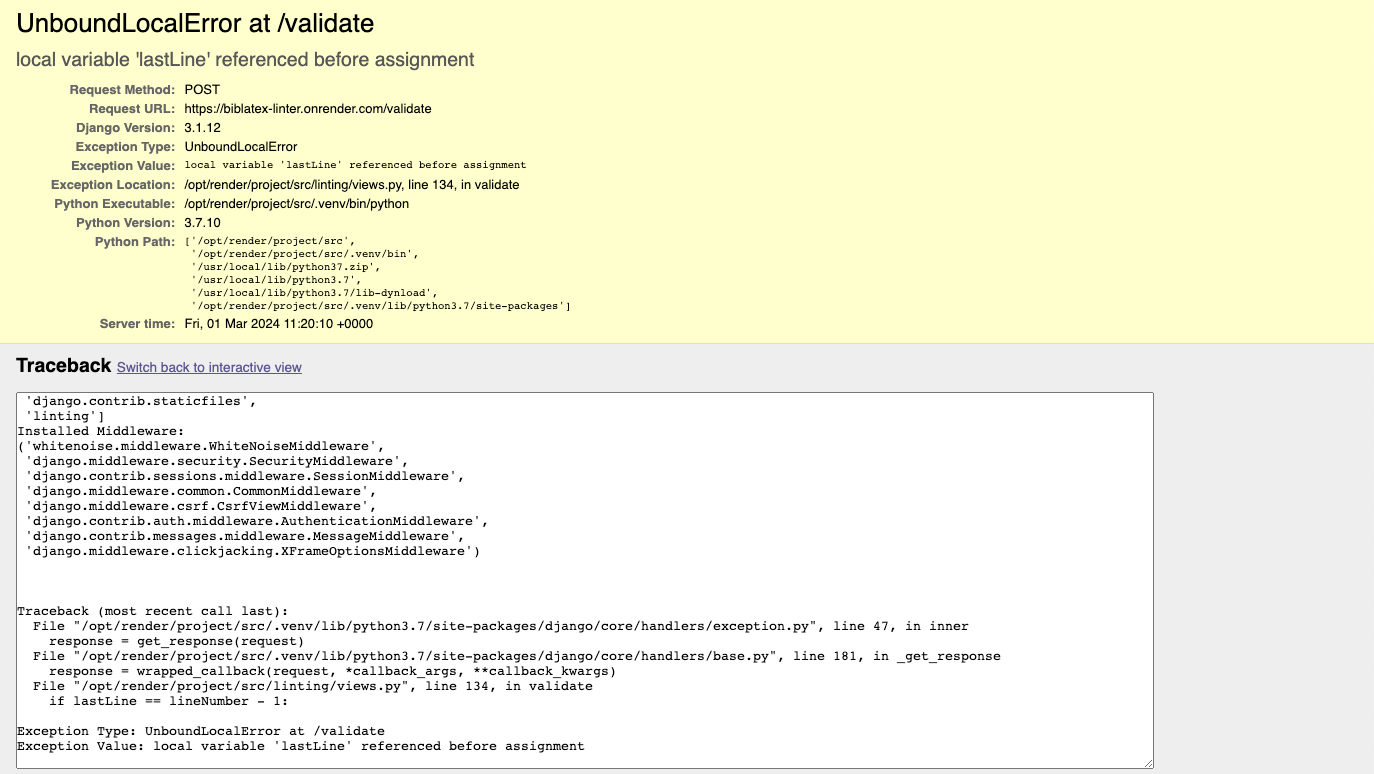
\includegraphics[width=0.7\textwidth]{./files/Pezmc-LinterError_cropped.png}
    \caption[Foutmelding BibLaTeX-linter]{Lintingerror bij het valideren van een BibLaTeX bestand, gebruikmakende van de linter geschreven door Pez Cuckow\footnote[1]{\ref{foot:pezgithub}}.}
    \label{fig:biblatex-linter-error}
\end{figure}

Daarnaast leek de aanpak van de geschreven code ook niet optimaal te zijn op vlak van leesbaarheid en uitbreidbaarheid. Gezien dit echter wel criteria zijn waar de proof of concept aan moest voldoen, werd er besloten om deze linter niet verder te onderzoeken. Er werd wel gekeken naar de functionaliteiten die deze linter aanbood en andere zaken die handig leken om over te nemen in de eigen implementatie.

\section{Andere linters}
Gezien het wat BibLaTeX linters betreft zeer beperkt is, werd er op zoek gegaan naar andere soorten linters. Bijvoorbeeld een linter voor JavaScript, Python of andere programmeertalen. Er werd gekeken naar het soort features dat de linters aanbieden, hun performantie, alsook als hun broncode indien deze toegankelijk was. Enkele linters die bekeken werden zijn: JSHint, Stylelint, Ruff, PyType en bibl. Net als de proof of concept, waren al de bekeken linters gratis te gebruiken en open source.

Daaruit bleek dat naast de manier van implementeren, de taal waaruit de linter opgebouwd is ook van belang is voor de performantie. Dit was het begin naar een onderzoek voor de ideale programmeertaal te vinden voor deze proof of concept. 

\subsection{Ruff}
% Ruff is een Python linter die door \textcite{Astral2024} ontwikkeld is. In vergelijking met andere Python linters is Ruff veel performanter. Dit is omdat Ruff in tegenstelling tot de concurrenten, geschreven is in Rust in plaats van Python. Op de website van Astral, makers van Ruff, is er een vergelijking te zien tussen Ruff en andere Python linters die wel in Python geschreven zijn. Astral is niet de enige die dit aantoont, ook \textcite{TurnerTrauring2023} schrijft in een artikel dat de snelheid van Ruff zeker merkbaar is en toont dit aan met behulp van uitgevoerde tests. Vooral bij pipelines op virtuele machines gezien deze vCPU's (virtuele processor units) gebruiken en deze meestal trager zijn dan de processing units die terug te vinden zijn in moderne laptops of desktops.
Ruff\footnote{\url{https://astral.sh/ruff}} is een Python linter ontwikkeld door \textcite{Astral2024}, geschreven in de programmeertaal Rust. Dit onderscheidt Ruff van andere Python linters, die doorgaans in Python zelf zijn geschreven. Rust staat bekend om zijn snelheid en veiligheid, wat het een uitstekende keuze maakt voor een linter. Bovendien is Rust lichter om op hardware te draaien dan Python, aangezien Python een interpretatieve taal is en Rust een gecompileerde taal. Dit maakt Ruff bijzonder geschikt voor gebruik in CI-pipelines. 

Een ander belangrijk voordeel van Rust is de stabiliteit van de taal. Er is slechts één versie van Rust en die wordt continu doorontwikkeld, wat ervoor zorgt dat code die vandaag gecompileerd wordt, ook over tien jaar nog gecompileerd kan worden. Dit biedt een aanzienlijke zekerheid voor de toekomstbestendigheid van software.

Ruff kan op bepaalde taken tien tot wel honderd keer sneller zijn dan zijn concurrenten. Dit wekt vanzelfsprekend de interesse om de prestaties van de Rust-taal te testen. Op de website van Astral, de makers van Ruff, is een vergelijking te vinden tussen Ruff en andere Python linters. Ook \textcite{TurnerTrauring2023} bevestigen in hun artikel dat de snelheid van Ruff duidelijk merkbaar is en onderbouwen dit met testresultaten. Deze prestaties zijn vooral voordelig in pipelines op virtuele machines, aangezien vCPU's (virtuele processor units) meestal trager zijn dan de verwerkingsunits in moderne laptops of desktops.

\subsection{DirtyRat}
\label{subsec:dirtyrat}
DirtyRat is een JavaScript linter waar op gebotst werd tijdens het onderzoeken naar hoe een linter gemaakt kon worden. Het is een linter die zelf in JavaScript geschreven is en waarvan de stapsgewijze opbouw te vinden is in het artikel van \textcite{BorgesLate2021}. Daarnaast is ook de broncode zelf te vinden op GitHub\footnote{\url{https://github.com/JoanaBLate/dirtyrat}}. Dit was ook de reden waarom er besloten werd om JavaScript als kandidaat-programmeertaal te nemen. 

Hoewel het artikel zeer in detail gaat en het grondig onderzocht werd, werd er vastgesteld dat het toch wat te uitgebreid is voor deze proof of concept. JavaScript en andere programmeertalen zitten met veel meer complexe structureren dan een BibLaTeX bestand. Dus hoewel het interessant was om te zien hoe een linter in JavaScript gemaakt kon worden, was het dus zeker niet nodig om elke component over te nemen.


\subsection{bibl}
bibl\footnote{\url{https://gitlab.com/arnevdk/bibl}} is een linter voor BibTeX, de voorloper van BibLaTeX, geschreven in Python door Arne Van Den Kerchove. Het onderzoeken van een linter voor de voorloper van BibLaTeX leek bijzonder interessant om een goed inzicht te krijgen in wat precies verwacht kan worden van een linter. bibl biedt een uitgebreide lijst van regels, evenals een gedetailleerde projectstructuur en implementatiewijze van zowel de lintercode als de bijbehorende tests.

bibl werd ontdekt net voordat er begonnen werd met de ontwikkeling van een eigen linter. Na een grondige analyse bleek dat bibl een goed opgebouwde, modulaire en efficiënte open-source linter is. bibl voldeed aan vrijwel alle criteria die voor de proof of concept linter waren opgesteld, wat leidde tot een nieuwe visie.

Het maken van een linter zoals bibl, maar dan voor BibLaTeX in plaats van BibTeX, leek een haalbaar einddoel. Echter, vanwege een achterstand op de planning, zou het niet mogelijk zijn om een eigen linter even uitgebreid uit te werken. Hoewel het concept van een proof of concept wellicht bereikt kon worden, leek het voordeliger om bibl te proberen gebruiken en compatibel te maken met BibLaTeX.

Gezien de verschillen tussen BibTeX en BibLaTeX, was er enige twijfel over de haalbaarheid hiervan, vooral omdat bibl gebruik maakt van pybtex als parser. Op de site van pybtex\footnote{\url{https://pybtex.org/}} staat het volgende vermeld:

\begin{quote}\emph{Pybtex is a BibTeX-compatible bibliography processor written in Python.}\end{quote}

Dit impliceert dat pybtex verantwoordelijk is voor het extraheren van gegevens uit bibliografiebestanden. Hoewel de quote niet expliciet vermeldt dat het alleen voor BibTeX-bestanden werkt, wordt compatibiliteit met BibLaTeX nergens expliciet genoemd. Het was dus noodzakelijk om dit zelf te testen.

Voor de test werd een BibLaTeX-document gebruikt dat door de promotor was gedeeld. Dit document bevatte geldige bronvermeldingen en was daarmee perfect geschikt om te onderzoeken of bibl als basis gebruikt kon worden. bibl werd snel geïnstalleerd via de Python package manager, pip. Vervolgens werd het lint-commando uitgevoerd op het BibLaTeX-document en werd bekeken wat bibl rapporteerde.

bibl crashte niet en genereerde een uitgebreide lijst opmerkingen; dit was een positief resultaat. Er waren echter enkele bestaande regels die niet compatibel waren met BibLaTeX-bestanden. 

\subsubsection{Algemene structuur}
\begin{figure}[ht]
    \centering
    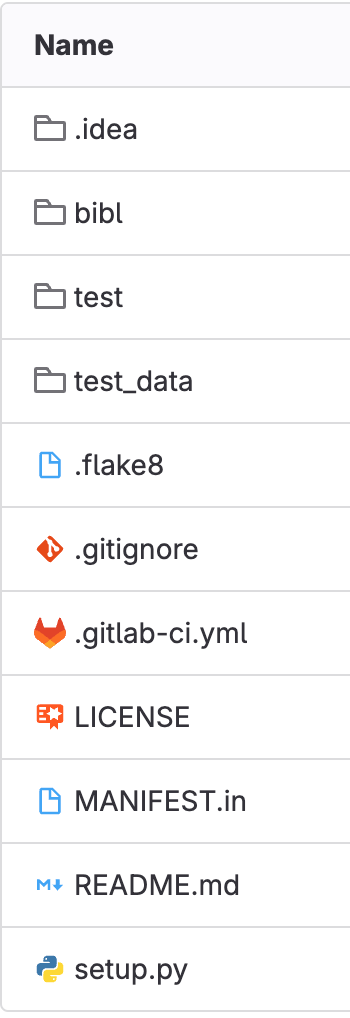
\includegraphics[width=0.3\textwidth]{./files/bibl_repo.png}
    \caption[bibl repository]{Repository overzicht bibl.}
    \label{fig:bibl_repo}
\end{figure}

De gitlab-repository van bibl\footnote{\url{https://gitlab.com/arnevdk/bibl}} is een goed voorbeeld van hoe een goed gestructureerd project eruit kan zien. Naast de bibl folder, die alle broncode van bibl zelf bevat, zijn er ook: testen, test-data, lintervoorkeuren, een pipeline (zie \ref{sec:pipelines}), een licentie, een duidelijke readme en een installatie-script aanwezig. Ook de .idea, .gitignore en MANIFEST.in zijn niet onbelangrijk. de .idea bevat de voorkeursinstellingen voor de IDE (Integrated development environment, ook gekend als werkomgeving) van de auteur, het .gitignore bestand bevat een opsomming van bestanden of soort bestanden die niet op de repository dienen te komen. Denk hier aan tijdelijke bestanden die vanzelf aangemaakt worden; deze zijn niet nodig op de repository omdat ze onnodig plaats gebruiken. Tot slot wordt het MANIFEST.in bestand in Python wordt gebruikt om aan te geven welke bestanden moeten worden opgenomen bij het maken van een distributiepakket; wat nodig is om het beschikbaar te stellen bij de pakketbeheerder\footnote{\url{https://pypi.org/}} (pip). In een latere sectie (\Ref{sec:bibl-in-depth}) wordt er dieper ingegaan op de volledige werking van de linter.
% ---
\section{Programmeertaal}

Om de gepaste programmeertaal te vinden, werden diverse kandidaat\babelhyphen{hard}programmeertalen overwogen. De kandidaat\babelhyphen{hard}programmeertalen waren: Rust, JavaScript en Python. Door het analyseren van reeds bestaande linters en het afgaan van een hele lijst aan programmeertalen, werd er besloten om met deze drie programmeertalen te experimenteren.

In een latere fase (sectie \ref{sec:mini-pocs}) werden er beperkte prototypes uitgewerkt in elk van deze talen; deze werden met elkaar vergeleken om te bepalen welke taal het meest geschikt zou zijn. Alle opties zijn cross-platform, wat belangrijk is gezien de linter bruikbaar dient te zijn voor iedereen. Alsook dient het een programmeertaal te zijn die gekend is, hiermee wordt er bedoeld dat het een programmeertaal moet zijn die al matuur is en door een groot aantal mensen gekend is.

\subsection{Rust}
Gezien de performantie van Ruff, leek Rust een gepaste optie om de linter in te maken. Ook de stijgende populariteit van de taal maakt dit een aantrekkelijke optie. Ondanks dat dit een onbekende taal is, leek het zeker wel een interessante taal om te leren. De haalbaarheid van de proof of concept kwam echter meer in gevaar door deze keuze. Hoewel de populariteit stijgt, blijft het wel nog een taal die niet door iedereen gekend is, in tegenstelling tot bijvoorbeeld JavaScript of Python. Een ander groot pluspunt aan Rust is dat code die vandaag compiled, ook nog binnen vijf of tien jaar zal kunnen compilen. Dit omdat de makers ervoor streven dat het een super compatibele programmeertaal is. Wat men niet met volle zekerheid van bijvoorbeeld Python\footnote{\url{https://devguide.python.org/versions/}} zou kunnen zeggen. 
 
Dankzij \textcite{Klabnik2022} kan er geleerd worden dat Rust een nadruk legt op typeveiligheid (typesafety) en geheugenveiligheid. Wanneer een taal of systeem geheugenveilig is, betekent dit dat het ontworpen is om toegangsfouten zoals bufferoverlopen, dangling pointers (verwijzingen naar vrijgegeven geheugen), en dubbele bevrijdingen van geheugen (double frees) te voorkomen. Deze soorten fouten kunnen leiden tot onvoorspelbaar gedrag, crashes, en beveiligingslekken zoals het uitvoeren van willekeurige code of informatie-lekken. Het is dus een goede eigenschap om te hebben.

\subsection{Python}
Python was wellicht stukken trager in vergelijking met Rust in de test die gevonden werd, maar het blijft wel een taal waar iedereen gemakkelijk mee kan beginnen te werken. Voor het gemak van uitbreidbaarheid is dit dan weer een interessante optie om deze taal in optie te nemen. Zoals eerder vermeld door \textcite{TurnerTrauring2023} zou de performantie vooral bij de pipeline te merken zijn.
De echte vraag blijft momenteel nog altijd in hoeverre het minder performant zijn een grote zorg zal worden voor deze proof of concept.

\subsection{JavaScript}
Een zeer gekende scripting taal dat cross-platform gebruikt kan worden. Hoewel het eerder gericht is voor het gebruik in websites of GUI gerichte scripts, is het ook mogelijk om er cli-tools mee te maken. De performantie werd onderzocht. JavaScript is ook een dynamisch typerende taal, wat in theorie voor problemen zou kunnen zorgen in sommige use-cases, al leek dit geen zorg te zijn voor deze proof of concept\autocite{Simpson2023}.

\section{Opbouw linter}
Aan het begin van dit project werd de beslissing genomen om direct met de ontwikkeling van een prototype aan de slag te gaan, wat leidde tot de zoektocht naar geschikte bronnen. Deze beslissing werd genomen gezien de beperkte tijd en de hoeveelheid aan onderzoek die diende te gebeuren. Indien Rust de taal zou moeten worden, moest deze nog volledig aangeleerd worden en zou er immers geen kostbare tijd verloren mogen gaan.

In dit proces werden de artikelen van \textcite{BorgesLate2021}, die een stapsgewijze handleiding bieden voor het bouwen van een JavaScript-linter, als bijzonder nuttig beschouwd. Ondanks dat de lectuur van deze serie aanvankelijk de indruk wekte dat het project complexer zou zijn dan verwacht, veranderde dit vermoeden na verder onderzoek naar de structuur van .bib-bestanden. Het werd duidelijk dat de ontwikkeling van een linter voor BibLaTeX minder complex is dan voor programmeertalen. Dit is te wijten aan het feit dat programmeertalen loops, conditionele statements en een scala aan andere complexe elementen bevatten, terwijl BibLaTeX gekenmerkt wordt door een consistente en gestandaardiseerde structuur, waardoor de noodzaak voor het opleggen van regels aanzienlijk vermindert. Het was echter wel zeer nuttig om alle componenten te zien die aan bod kunnen komen bij het bouwen van een linter en om deze in gedachte te houden voor de effectieve uitwerking van de BibLaTeX-linter proof of concept.


\section{bibl pakket - diepere blik}
\label{sec:bibl-in-depth}
\begin{figure}[ht]
    \centering
    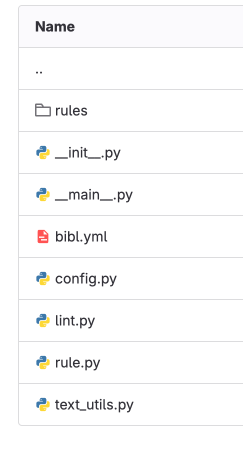
\includegraphics[width=0.4\textwidth]{./files/bibl_src.png}
    \caption[bibl repository - source code]{Repository overzicht bibl broncode.}
    \label{fig:bibl_src}
\end{figure}

De structuur van bibl \ref{fig:bibl_src} volgt een gebruikelijke pakket-gebaseerde aanpak voor het organiseren van code. Deze aanpak wordt vaak toegepast wanneer een project is opgezet als een herbruikbaar pakket, in plaats van een los script. De aanwezigheid van `\_\_init\_\_.py` zorgt er namelijk voor dat het pakket importeerbaar is \autocite{Loubser2021}. Dit is direct ook een indicator dat het om een pakket gaat.

Om bibl te begrijpen, wordt de broncode van bibl zelf geanalyseerd.

\subsection{\_\_init\_\_.py}
Zoals eerder vermeld, is dit bestand kenmerkend bij pakketten. Het bestand is namelijk vereist voor Python om de directory als een pakket te behandelen. Het kan leeg zijn, maar het kan ook initialisatiecode of pakket-niveau-definities bevatten; in dit geval bevat het de huidige softwareversie.

\subsection{\_\_main\_\_.py}
Dit bestand wordt gebruikt wanneer het pakket als een script wordt uitgevoerd (bijvoorbeeld python -m bibl). Het bevat de implementatie van de Command Line Interface (CLI) voor het linten van bibliografische bestanden in BibTeX-formaat. Het script, hiervoor als referentie bestand, maakt gebruik van de \texttt{Click}-bibliotheek om een gebruiksvriendelijke interface te bieden voor het controleren van bibliografische referenties op consistentie en correctheid. Hieronder volgt een overzicht van de verschillende onderdelen binnen dit bestand.

\subsubsection{Imports en Configuratie}

Het script begint met het importeren van noodzakelijke modules en functies, waaronder \texttt{Click} voor het CLI-framework, en functies uit de \texttt{bibl}-module voor linting, configuratie en regels:

\begin{minted}[autogobble, breaklines, linenos, samepage]{python3}
import os
import warnings
import click
from bibl import __version__
from bibl.lint import lint as bibl_lint
from bibl.config import load_config_file, set_config
from bibl.rule import load_rules
from bibl.text_utils import format_rules_markdown_tables
\end{minted}

\subsubsection{CLI Basisgroep}

Een CLI basisgroep functioneert als een container, of groepering, voor meerdere gerelateerde command-line commando's. Hiermee wordt het mogelijk gemaakt om een hoofdcommando te definiëren waaraan subcommando's kunnen worden toegevoegd.
De basisgroep wordt gedefinieerd met behulp van de \texttt{@click.group()} decorator. Deze groep fungeert als een container voor subcommando's die specifieke taken uitvoeren. De subcommando's kunnen tegelijkertijd ook als parameter beschouwd worden. Opties die van toepassing zijn op de gehele groep kunnen hier ook worden gespecificeerd. Een voorbeeld van de definitie van een basisgroep in het script is als volgt:

\begin{minted}[autogobble, breaklines, linenos]{python3}
@click.group()
@click.option('-c', '--config', help='Custom configuration file path.', type=str)
@click.option('--select', help='Comma separated list of enabled rules, all other rules will be disabled.', type=str)
@click.option('--ignore', help='Comma separated list of disabled rules, all other rules will be enabled.', type=str)
@click.option('--indent-spaces', help='Number of trailing whitespaces for indented line, used by TO1.', type=int)
@click.option('--max-line-length', help='Max line length before wrap recommended, used by T03.', type=int)
def cli(config, select, ignore, indent_spaces, max_line_length):
    if config is not None:
        load_config_file(config)
    elif os.path.isfile('bibl.yml'):
        load_config_file('bibl.yml')
    elif os.path.isfile('.bibl.yml'):
        load_config_file('.bibl.yml')
    if select is not None:
        set_config('select', select.split(','))
    if ignore is not None:
        set_config('ignore', ignore.split(','))
    set_config('indent_spaces', indent_spaces)
    set_config('max_line_length', max_line_length)
\end{minted}

\subsubsection{Lint Commando}

Het \texttt{lint} commando lint één of meer opgegeven BibTeX-bestanden:

\begin{minted}[autogobble, breaklines, linenos, samepage]{python3}
@cli.command(help="Lint a BibTeX bibliography file.")
@click.argument('bibliography', type=str, nargs=-1)
def lint(bibliography):
    warnings.filterwarnings("ignore")
    for bib in bibliography:
        bibl_lint(bib)
\end{minted}

\subsubsection{Lijst Commando's}

Er zijn twee commando's om de lintingregels weer te geven: \texttt{list\_all} toont alle beschikbare regels, terwijl \texttt{list\_enabled} alleen de ingeschakelde regels toont.

\begin{minted}[autogobble, breaklines, linenos]{python3}
@cli.command(help="Show all available rules.")
@click.option('-m', 'markdown', help='Format rules as markdown table.', is_flag=True)
def list_all(markdown):
    rules = load_rules().all
    if markdown:
        click.echo(format_rules_markdown_tables(rules))
    else:
        for rule in rules:
            click.echo(rule)

@cli.command(help="Show all rules enabled by the configuration.")
@click.option('-m', 'markdown', help='Format rules as markdown table.', is_flag=True)
def list_enabled(markdown):
    rules = load_rules().enabled
    if markdown:
        click.echo(format_rules_markdown_tables(rules))
    else:
        for rule in rules:
            click.echo(rule)
\end{minted}

\subsubsection{Versie Commando}

Het \texttt{version} commando toont de huidige versie van het \texttt{bibl}-pakket:

\begin{minted}[autogobble, breaklines, linenos, samepage]{python3}
@cli.command(help="Show the package version.")
def version():
    click.echo('bibl version: ' + __version__)
\end{minted}

\subsubsection{Hoofdprogramma}

Het hoofdprogramma start de CLI met \texttt{cli(prog\_name='bibl')}:

\begin{minted}[autogobble, breaklines, linenos, samepage]{python3}
if __name__ == '__main__':
    cli(prog_name='bibl')
\end{minted}
%---
\subsection{bibl.yml - Configuratiebestand}
Het volgende configuratiebestand is een YAML (.yml) bestand dat de standaardinstellingen voor de bibliografische lintingtool definieert. Dit bestand specificeert welke regels ingeschakeld of uitgeschakeld moeten worden, evenals andere configuratie-opties zoals de maximale regellengte en het aantal inspringende spaties.

\begin{minted}[autogobble, breaklines, linenos]{yaml}
## DEFAULT BIBL CONFIG
select: [ ] # List of enabled rules, all other rules will be disabled
ignore: [ ] # List of disabled rules, all other rules will be enabled
# Specify max 1 of the two options above. If none are specified, all rules will be enabled
indent_spaces: 4 # number of trailing whitespaces for indented line, used by TO1
max_line_length: 120  # max line length before wrap recommended, used by T03
abbreviation_dot: True  # abbreviate middle names with dot (John F. Kennedy) as opposed to without (John F Kennedy), used by E02

# Specification from https://en.wikipedia.org/wiki/BibTeX extended with fields used in JabRef.
# This specification is used to generate M01 and U01 rules
type_spec:
  article: # An article from a journal or magazine.
    required: [ title, journal, year, volume ]
    optional: [ number, pages, month, doi, key, file ]
  book: # A book with an explicit publisher.
    required: [ title, publisher, year ]
    optional: [ volume, number, series, address, edition, month, key, url, file, isbn ]
# NOTE: Overige entry types weggelaten wegens plaats!
\end{minted}

\subsubsection{Beschrijving van de Configuratieopties}

De YAML-configuratie begint met het definiëren van een aantal algemene opties voor de linter:

\begin{itemize}
    \item \texttt{select}: Een lijst van ingeschakelde regels. Indien gespecificeerd, worden alle andere regels uitgeschakeld.
    \item \texttt{ignore}: Een lijst van uitgeschakelde regels. Indien gespecificeerd, worden alle andere regels ingeschakeld.
    \item \texttt{indent\_spaces}: Het aantal inspringende spaties voor ingesprongen regels, gebruikt door de regel TO1.
    \item \texttt{max\_line\_length}: De maximale regellengte voordat een regel wordt afgebroken, aanbevolen door de regel T03.
    \item \texttt{abbreviation\_dot}: Bepaalt of middelste namen met een punt worden afgekort (bijvoorbeeld John F. Kennedy) of zonder punt (bijvoorbeeld John F Kennedy), gebruikt door de regel E02.
\end{itemize}

\subsubsection{Type Specificaties}

Daarnaast bevat het configuratiebestand een specificatie van verschillende typen BibTeX-entries en hun vereiste en optionele velden. Deze specificatie is gebaseerd op de standaard BibTeX-specificatie en is uitgebreid met velden die worden gebruikt in JabRef. Deze specificatie wordt gebruikt om de regels M01 en U01 te genereren.
Hieronder zijn er enkelen opgelijst, maar let op, het zijn ze niet allemaal! Raadpleeg de gehele lijst op de GitLab-repository van bibl\footnote{\url{https://gitlab.com/arnevdk/bibl/-/blob/master/bibl/bibl.yml}}
\begin{itemize}
    \item \texttt{article}: Een artikel uit een tijdschrift of magazine. Vereist velden zoals \texttt{title}, \texttt{journal}, \texttt{year}, en \texttt{volume}.
    \item \texttt{book}: Een boek met een expliciete uitgever. Vereist velden zoals \texttt{title}, \texttt{publisher}, en \texttt{year}.
    \item \texttt{booklet}: Een werk dat is gedrukt en gebonden, maar zonder een genoemde uitgever of sponsorende instelling. Vereist het \texttt{title} veld.
    \item ...
\end{itemize}

Deze configuratie-instellingen en type-specificaties vormen de basis voor het configureren en uitvoeren van de bibliografische lintingtool, waarbij consistentie en correctheid van de bibliografische gegevens worden gewaarborgd.

% --------------
\subsection{config.py - Configuratielogica}

De volgende code implementeert de logica voor het laden en beheren van configuratie-instellingen voor de bibliografische lintingtool. Deze configuratie-instellingen worden gedefinieerd in een YAML-bestand en geladen bij de initialisatie van de linter.

\begin{minted}[autogobble, breaklines, linenos]{python}
"""Linter configuration logic."""
from typing import Dict, Any

import pkg_resources
import yaml

_config = dict()
_read_default = False

_DEFAULT_CONFIG_FILE = 'bibl.yml'


def get_config() -> Dict:
    """Return the loaded config or instantiate and return default config."""
    if not _read_default:
        _load_default_config()
    return _config


def set_config(key: str, value: Any, default: bool = False):
    """Set a value in the configurations.

    :param key: configuration entry key
    :param value: configuration entry value
    :param default: If true, set as default value to be overwritten by later
    """
    if value is not None:
        if default:
            _config.setdefault(key, value)
        else:
            _config[key] = value
        _validate_and_clean_config(_config)


def load_config_file(file):
    """Read a YAML config file and use it as the configuration.

    :param file: .yaml config file path
    """
    with open(file) as config_file:
        config = yaml.load(config_file, Loader=yaml.FullLoader)
        for k, v in config.items():
            set_config(k, v)


def _load_default_config():
    global _read_default
    _read_default = True
    with open(pkg_resources.resource_filename(__name__,
                                              _DEFAULT_CONFIG_FILE)) as \
            default_config_file:
        default_config = yaml.load(default_config_file, Loader=yaml.FullLoader)
        for k, v in default_config.items():
            set_config(k, v, default=True)


def _validate_and_clean_config(config):
    if 'select' in config and 'ignore' in config and config['select'] and \
            config['ignore']:
        raise ValueError(
            "Configuration cannot contain both included and selected and "
            "ignored rules. Use either include or exclude to select"
            "enabled rules."
        )
\end{minted}

\subsubsection{Beschrijving van de Functies}

\begin{itemize}
    \item \texttt{get\_config}: Retourneert de geladen configuratie of instantieert en retourneert de standaardconfiguratie indien deze nog niet is geladen.
    \item \texttt{set\_config}: Stelt een waarde in de configuraties in. Indien de parameter \texttt{default} waar is, wordt de waarde alleen ingesteld als deze nog niet bestaat. Deze functie valideert en reinigt ook de configuratie.
    \item \texttt{load\_config\_file}: Leest een YAML-configuratiebestand en gebruikt deze als de huidige configuratie. Elk configuratie-item wordt ingesteld met behulp van de \texttt{set\_config} functie.
    \item \texttt{\_load\_default\_config}: Laadt de standaardconfiguratie vanuit het standaard configuratiebestand (\texttt{bibl.yml}). Deze functie wordt aangeroepen bij de eerste toegang tot de configuratie.
    \item \texttt{\_validate\_and\_clean\_config}: Valideert de configuratie door te controleren of niet zowel de \texttt{select} als de \texttt{ignore} opties tegelijk zijn gespecificeerd. Indien beide zijn gespecificeerd, wordt een \texttt{ValueError} opgeworpen.
\end{itemize}

\subsubsection{Toepassing en Validatie}

De configuratielogica zorgt ervoor dat de linter correct wordt ingesteld volgens de specificaties van de gebruiker, zoals gedefinieerd in een YAML-configuratiebestand. De standaardconfiguratie wordt geladen bij de eerste toegang tot de configuratie om ervoor te zorgen dat de linter altijd met geldige instellingen werkt. Daarnaast wordt de configuratie gevalideerd om conflicterende instellingen te voorkomen, zoals het gelijktijdig gebruik van \texttt{select} en \texttt{ignore}.

Deze gestructureerde benadering voor het laden en beheren van configuraties helpt bij het waarborgen van de consistentie en flexibiliteit van de linter, waardoor gebruikers specifieke instellingen kunnen aanpassen aan hun behoeften zonder de integriteit van het systeem in gevaar te brengen.
% --
\subsection{lint.py - Hoofdlogica}

De hoofdlogica van bibl bevindt zich in liny.py. 
Hier gebeuren de controles van de bibliografische referenties, zowel consistentie als correctheid worden gecontroleerd op basis van de opgestelde regels.

\begin{minted}[autogobble, breaklines, linenos]{python}
"""Main linter logic."""
import logging
import sys
from dataclasses import dataclass
from typing import List, Iterable

import pybtex
from pybtex.database import parse_file
from bibl.rule import load_rules, Rule, EntryRule, TextRule
from bibl.text_utils import find_entry_line_number, MONTH_NAMES

logger = logging.getLogger()
logger.setLevel(logging.WARNING)

handler = logging.StreamHandler(sys.stdout)
handler.setLevel(logging.WARNING)
logger.addHandler(handler)


@dataclass
class LintWarning:
    """Dataclass to represent and report a linter rule violation."""

    # file path of the detected violation
    file: str
    # line number of the detected violation
    line: int
    # the violated rule
    rule: Rule

    def log(self):
        """Print the warning with details to stdout."""
        msg = "{}:{} {}".format(self.file, self.line, str(self.rule))
        logger.warning(msg)


def lint(bibliography: str, verbose: bool = True) -> List[LintWarning]:
    """Execute the main linter program.

    The linter will first scan the bibliography text file and check all text
    rules for each line in the text file. Next, the file will be parsed by the
    pybtex parser and all entry rules will be checked.

    :param bibliography: a .bib bibliography file path
    :param verbose: log linter warnings to stdout
    :return: a list of LintWarning objects representing the linter violations
    found while running
    """
    bib_data = parse_file(bibliography, macros=MONTH_NAMES)
    bib_data.file = bibliography
    with open(bibliography, 'r') as bib_file:
        bib_text = bib_file.read()

    rules = load_rules()

    text_warnings = _apply_text_rules(bibliography, bib_text,
                                      rules.enabled_text_rules)
    entry_warnings = _apply_entry_rules(bibliography, bib_data, bib_text,
                                        rules.enabled_entry_rules)

    warnings = text_warnings + entry_warnings

    warnings.sort(key=lambda w: w.rule.rule_id)
    warnings.sort(key=lambda w: w.line)
    if verbose:
        for warning in warnings:
            warning.log()
    return warnings


def _apply_text_rules(bibliography: str, bib_text: str,
                      text_rules: Iterable[TextRule]) -> List[LintWarning]:
    """Check all text rules in the bibliography text file.

    :param bibliography: bibliography file path
    :param bib_text: bibliography file contents
    :param text_rules: list of text rules to be evaluated on each line of
    the file
    :return: a list of LinterWarnings representing found rule violations
    """
    warnings = []
    for i, line in enumerate(bib_text.split('\n')):
        line_number = i + 1
        for rule in text_rules:
            result = rule(line_number, line, bib_text)
            if not result:
                warnings.append(LintWarning(bibliography, line_number, rule))
    return warnings


def _apply_entry_rules(bibliography: str,
                       bib_data: pybtex.database.BibliographyData,
                       bib_text: str, entry_rules: Iterable[EntryRule]) \
        -> List[LintWarning]:
    """Check all entry rules in the bibliography text file.

    :param bibliography: bibliography file path
    :param bib_data: parsed bibliography data containing entries
    :param bib_text: bibliography file contents
    :param entry_rules: list of entry rules to be evaluated on each entry
    :return: a list of LintWarning representing found rule violations
    """
    warnings = []
    for key, entry in bib_data.entries.items():
        for rule in entry_rules:
            line_number, offset = find_entry_line_number(bib_text, key)
            result = rule(key, entry, bib_data)
            if not result:
                warnings.append(LintWarning(bibliography, line_number, rule))
    return warnings
\end{minted}

\subsubsection{Beschrijving van de Functies}

\begin{itemize}
    \item \texttt{LintWarning}:
    Een dataclass die een lintingwaarschuwing vertegenwoordigt. Deze bevat de volgende attributen:
    \begin{itemize}
        \item \texttt{file}: Het pad naar het bestand waarin de overtreding is gedetecteerd.
        \item \texttt{line}: Het regelnummer van de gedetecteerde overtreding.
        \item \texttt{rule}: De overtreden regel.
    \end{itemize}
    De \texttt{log} methode wordt gebruikt om de waarschuwing met details naar stdout te loggen.

    \item \texttt{lint}:
    Voert het hoofdprogramma van de linter uit. De functie controleert eerst de bibliografietekst op alle tekstregels voor elke regel in de tekst. Vervolgens wordt het bestand geparseerd met de pybtex parser en worden alle invoerregels gecontroleerd.
    \begin{itemize}
        \item \texttt{bibliography}: Het pad naar een .bib bibliografisch bestand.
        \item \texttt{verbose}: Logt linterwaarschuwingen naar stdout indien ingesteld op \texttt{True}.
        \item Retourneert een lijst van \texttt{LintWarning} objecten die de tijdens het uitvoeren gevonden overtredingen vertegenwoordigen.
    \end{itemize}

    \item \texttt{\_apply\_text\_rules}:
    Controleert alle tekstregels in het bibliografietekstbestand.
    \begin{itemize}
        \item \texttt{bibliography}: Het pad naar het bibliografisch bestand.
        \item \texttt{bib\_text}: De inhoud van het bibliografiebestand.
        \item \texttt{text\_rules}: Een lijst van tekstregels die op elke regel van het bestand worden geëvalueerd.
        \item Retourneert een lijst van \texttt{LintWarning} objecten die gevonden overtredingen van de tekstregels vertegenwoordigen.
    \end{itemize}

    \item \texttt{\_apply\_entry\_rules}:
    Controleert alle invoerregels in het bibliografietekstbestand.
    \begin{itemize}
        \item \texttt{bibliography}: Het pad naar het bibliografisch bestand.
        \item \texttt{bib\_data}: Geparste bibliografische gegevens die entries bevatten.
        \item \texttt{bib\_text}: De inhoud van het bibliografiebestand.
        \item \texttt{entry\_rules}: Een lijst van invoerregels die op elke entry worden geëvalueerd.
        \item Retourneert een lijst van \texttt{LintWarning} objecten die gevonden overtredingen van de invoerregels vertegenwoordigen.
    \end{itemize}
\end{itemize}

\subsubsection{Logica en Validatie}

De hoofdlogica van de linter begint met het instellen van de loggingconfiguratie om waarschuwingen naar stdout te sturen. Vervolgens worden de regels voor de linter geladen en toegepast op de bibliografische gegevens. Er wordt eerst gekeken naar overtredingen in de tekstregels, gevolgd door overtredingen in de invoerregels. De gevonden overtredingen worden gesorteerd op regel-ID en regelnummers, en indien de \texttt{verbose} parameter is ingesteld, worden deze overtredingen gelogd naar stdout. Deze aanpak zorgt voor een gestructureerde controle van bibliografische bestanden, waarbij consistentie en correctheid worden gewaarborgd.

% ---
\subsection{rule.py - Structuur voor het Beheren van Regels}

De volgende code implementeert een structuur voor het beheren van lintingregels op een uniforme manier. Deze structuur maakt het mogelijk om regels te definiëren, registreren en evalueren binnen bibl.

\subsubsection{De \texttt{Rule} Klasse}

De \texttt{Rule} klasse is een generieke klasse voor een lintingregel. Deze klasse bevat attributen voor het identificeren en beschrijven van de regel, evenals een \emph{callable} om de regel te controleren. Een \emph{callable} is een object dat kan worden aangeroepen als een functie.

\begin{minted}[autogobble, breaklines, linenos]{python}
import fnmatch
import os
from typing import Callable, Dict, List
from pybtex.database import Entry
from bibl.config import get_config

class Rule:
    """Generic rule class.

    :param rule_id: identifying code for this rule, starting with a letter
    indicating the rule type, followed by a number or a string specification.
    :param description: a full sentence description of the rule
    """

    def __init__(self, rule_id: str, description: str, rule: Callable):
        """Create Rule object.

        :param rule_id: identifying code for this rule, starting with a letter
        indicating the rule type, followed by a number or a string
        specification.
        :param description: a full sentence description of the rule
        :param rule: a callable returning a boolean to execute when checking
        this rule
        """
        self.rule_id = rule_id
        self.description = description
        self._rule = rule

    def __str__(self):
        """Return rule as string representation."""
        return "{}: {}".format(self.rule_id, self.description)

    def __call__(self, *args, **kwargs):
        """Handle Rule objects as callables.

        When calling a rule, it is evaluated over (a part of) the bibliography.
        :param args, kwargs: Rule arguments
        :return: True if the bibliography is consistent with the rule, False if
        the rule is violated.
        """
        return self._rule(*args, **kwargs)

    @property
    def enabled(self):
        """Evaluate wheter a rule should be checked this run.

        :return: True if the rule should be checked based on the configuration
        used for running the linter, False otherwise
        """
        if get_config()['select']:
            for pattern in get_config()['select']:
                if fnmatch.fnmatch(self.rule_id, pattern):
                    return True
            return False
        if get_config()['ignore']:
            for pattern in get_config()['ignore']:
                if fnmatch.fnmatch(self.rule_id, pattern):
                    return False
            return True
        return True
\end{minted}

\subsubsection{De \texttt{EntryRule} en \texttt{TextRule} Klassen}

De \texttt{EntryRule} en \texttt{TextRule} zijn subklassen van \texttt{Rule}. \texttt{EntryRule} wordt gebruikt om regels te evalueren op geparseerde bibliografie-entries, terwijl \texttt{TextRule} wordt gebruikt om regels te evalueren op tekstregels in bibliografie-entries.

\begin{minted}[autogobble, breaklines, linenos]{python}
class EntryRule(Rule):
    """Rule type evaluating a parsed bibliography entry."""

    def __init__(self, rule_id, description,
                 rule: Callable[[str, Entry, Dict[str, Entry]], bool]):
        """Create EntryRule object.

        :param key: The key of the current bibliography entry
        :param entry: The current bibliography entry
        :param database: All bibliography entries
        """
        super().__init__(rule_id, description, rule)


class TextRule(Rule):
    """Rule type evaluating a text line in the bibliography entry."""

    def __init__(self, rule_id, description,
                 rule: Callable[[int, str, str], bool]):
        """Create TextRule object.

        :param line_number: The number of the current line in the bibliography
        :param line: The content of the current line in the bibliography
        :param text: The entire bibliography
        """
        super().__init__(rule_id, description, rule)
\end{minted}

\subsubsection{De \texttt{RuleStore} Klasse}

De \texttt{RuleStore} klasse dient als container voor alle geladen regels. Deze klasse bevat methoden om regels te registreren en op te halen.

\begin{minted}[autogobble, breaklines, linenos]{python}
class RuleStore:
    """Container for all loaded rules."""

    def __init__(self):
        """Create RuleStore object."""
        self._rules = []

    def register(self, rule: Rule):
        """Register a new rule.

        :param: a Rule object to register
        """
        position = 0
        while position < len(self._rules) \
                and self._rules[position].rule_id < rule.rule_id:
            position += 1
        self._rules.insert(position, rule)

    @property
    def all(self) -> List[Rule]:
        """Return all loaded rules."""
        return self._rules

    @property
    def enabled(self) -> List[Rule]:
        """Return all loaded rules enabled by the configuration."""
        return [rule for rule in self._rules if rule.enabled]

    @property
    def enabled_entry_rules(self) -> List[EntryRule]:
        """Return all loaded entry rules."""
        return [rule for rule in self.enabled if isinstance(rule, EntryRule)]

    @property
    def enabled_text_rules(self) -> List[TextRule]:
        """Return all loaded text rules."""
        return [rule for rule in self.enabled if isinstance(rule, TextRule)]
\end{minted}

\subsubsection{Registratie en Laden van Regels}

Door gebruik te maken van het decorator design patroon, zie \texttt{register\_entry\_rule} en \texttt{register\_text\_rule}, kunnen nieuwe regels eenvoudig worden toegevoegd aan de linter. De \texttt{load\_rules} functie importeert automatisch alle modules in het \texttt{bibl/rules} pakket, waardoor alle daarin gedefinieerde regels automatisch worden geladen en geregistreerd.

\begin{minted}[autogobble, breaklines, linenos]{python}
_ALL_RULES: RuleStore = RuleStore()

def register_entry_rule(rule_id, description: str) -> Callable:
    """Register a function as an entry rule."""
    def decorator(f: Callable[[str, Entry, Dict[str, Entry]], bool]):
        rule = EntryRule(rule_id, description, f)
        _ALL_RULES.register(rule)
    return decorator

def register_text_rule(rule_id: str, description: str) -> Callable:
    """Register a function as a text rule."""
    def decorator(f: Callable[[int, str, str], bool]):
        rule = TextRule(rule_id, description, f)
        _ALL_RULES.register(rule)
    return decorator

def load_rules() -> RuleStore:
    """Import all modules in the `bibl/rules` package."""
    for module in os.listdir(os.path.join(os.path.dirname(__file__), 'rules')):
        if module == '__init__.py' or module[-3:] != '.py':
            continue
        __import__('bibl.rules.' + module[:-3], locals(), globals())
    del module
    return _ALL_RULES
\end{minted}

\subsubsection{Logica en Validatie}

De structuur begint met het importeren van de benodigde modules en het definiëren van de \texttt{Rule} klasse, die de basis vormt voor alle regels. Vervolgens worden de \texttt{EntryRule} en \texttt{TextRule} subklassen gedefinieerd voor respectievelijk invoer- en tekstregels. De \texttt{RuleStore} klasse dient als container voor alle geregistreerde regels en biedt methoden om deze op te halen en te filteren op basis van de huidige configuratie.

Door gebruik te maken van decorators zoals \texttt{register\_entry\_rule} en \texttt{register\-\_text\-\_rule}, kunnen nieuwe regels eenvoudig worden toegevoegd aan de linter. De \texttt{load\_rules} functie importeert automatisch alle modules in het \texttt{bibl/rules} pakket, waardoor alle daarin gedefinieerde regels automatisch worden geladen en geregistreerd.

Deze aanpak zorgt voor een flexibele en uitbreidbare structuur voor het beheren van lintingregels, waardoor de consistentie en correctheid van bibliografische gegevens gewaarborgd blijven. Dit is van groot belang om bibl als basis te kunnen zien voor de eigen linter die uitgewerkt zal worden.

% ----
\subsection{text\_utils.py - Helper Functies voor Tekstverwerking}

In dit bestand staan helperfuncties voor tekstverwerking gedefinieerd die worden gebruikt door de lintingregels en andere commando's. Deze functies helpen bij het vinden van regelnummers, het formatteren van regels als Markdown-tabellen en andere tekstverwerkingsactiviteiten.

\subsubsection{Importeren van Noodzakelijke Modules}

Net gelijk bij de andere componenten, worden er ook hier eerst de benodigde modules en bibliotheken geïmporteerd. In dit geval zijn dit: reguliere expressies, typing voor typeannotaties, en een externe bibliotheek voor het genereren van Markdown-tabellen.

\begin{minted}[autogobble, breaklines, linenos]{python}
import re
from typing import List

import markdown_table

# Month name dictionary for pybtex
from bibl.rule import Rule

MONTH_NAMES = {
    'jan': 'jan',
    'feb': 'feb',
    'mar': 'mar',
    'apr': 'apr',
    'may': 'may',
    'jun': 'jun',
    'jul': 'jul',
    'aug': 'aug',
    'sep': 'sep',
    'oct': 'oct',
    'nov': 'nov',
    'dec': 'dec'
}
\end{minted}

De declaratie van \texttt{MONTH\_NAMES} (regel 9 en volgende) zorgt voor een gestandaardiseerde verwerking van maandnamen in bibliografische gegevens. Dit biedt consistentie, eenvoudige toegang, compatibiliteit met externe bibliotheken zoals in dit geval \texttt{pybtex}, en verbetert de leesbaarheid en onderhoudbaarheid van de code.

\subsubsection{Functie \texttt{find\_match\_line\_number}}

De functie \texttt{find\_match\_line\_number} wordt gebruikt om het regelnummer en de \emph{offset}, het aantal karakters vanaf het begin van de tekst, van een regex-match in een gegeven tekst te vinden.

\begin{minted}[autogobble, breaklines, linenos]{python}
def find_match_line_number(text: str, pattern: str, group: int) -> (int, int):
    r"""Find the line number and offset of a regex match.

    :param text: text to match
    :param pattern: regex pattern
    :param group: regex group number of the intended match
    :return: Line number (based on \n characters) of first occurrence of the
    specified match, offset of the first occurrence of the match in the line
    """
    regex = re.compile(pattern)
    match = next(regex.finditer(text))
    start = match.start(group)
    lineno = text.count('\n', 0, start)
    if lineno:
        offset = start - text.rfind('\n', 0, start)
    else:
        offset = start
    return lineno + 1, offset + 1
\end{minted}

\subsubsection{Functie \texttt{find\_entry\_line\_number}}

De functie \texttt{find\_entry\_line\_number} wordt gebruikt om het regelnummer van een BibTeX-entry in een gegeven tekst te vinden op basis van de entry-sleutel.

\begin{minted}[autogobble, breaklines, linenos]{python}
def find_entry_line_number(text: str, key: str) -> (int, int):
    r"""Find the file line number of a pybtex entry.

    :param text: BibTeX file string
    :param key: Entry key
    :return: Line number (based on \n characters) of first occurrence of the
    entry key, offset of the first occurrence of the key in the line
    """
    pattern = r'\s*@[a-zA-Z]+\s*{\s*(' + key + r')\s*,'
    return find_match_line_number(text, pattern, 1)
\end{minted}

\subsubsection{Functie \texttt{format\_rules\_markdown\_tables}}

De functie \texttt{format\_rules\_markdown\_tables} wordt gebruikt om een lijst van lintingregels als een Markdown-tabel te formatteren.

\begin{minted}[autogobble, breaklines, linenos]{python}
def format_rules_markdown_tables(rules: List[Rule]) -> str:
    """Format a list of bibl rules as a Markdown table.

    :param: rules: a list of Rule instances
    :return: A string containing a markdown table of human readable rules
    """
    result = "# bibl rules\n"
    headers = ["Rule ID", "Rule description"]
    matrix = []
    for i, rule in enumerate(rules):
        if i != 0 and rule.rule_id[0] != rules[i - 1].rule_id[0]:
            result += "## " + rules[i - 1].rule_id[0]
            result += "\n"
            result += markdown_table.render(headers, matrix)
            result += "\n\n"
            matrix = []
        matrix.append([f'`{rule.rule_id}`', rule.description])
    result += "## " + rule.rule_id[0]
    result += "\n"
    result += markdown_table.render(headers, matrix)
    return result
\end{minted}

\subsubsection{Beschrijving van de Functies}

\begin{itemize}
    \item \texttt{find\_match\_line\_number}: Deze functie zoekt naar een regex-match in de tekst en retourneert het regelnummer en de offset van de eerste match. Dit is nuttig voor het lokaliseren van specifieke patronen binnen een tekst.
    \item \texttt{find\_entry\_line\_number}: Deze functie zoekt naar het regelnummer van een BibTeX-entry op basis van de gegeven entry-sleutel. Dit helpt bij het vinden van specifieke bibliografische items binnen een BibTeX-bestand.
    \item \texttt{format\_rules\_markdown\_tables}: Deze functie neemt een lijst van \texttt{Rule} objecten en formatteert deze als een Markdown-tabel. Dit maakt het mogelijk om regels op een leesbare en georganiseerde manier weer te geven\footnote{\url{https://arnevdk.gitlab.io/-/bibl/-/jobs/952978205/artifacts/all_rules.html}}.
\end{itemize}

\subsubsection{Gebruik van Externe Bibliotheken}

De functies maken gebruik van verschillende externe bibliotheken:
\begin{itemize}
    \item \texttt{re}: Voor het werken met reguliere expressies.
    \item \texttt{markdown\_table}: Voor het genereren van Markdown-tabellen.
    \item \texttt{pybtex}: Voor het werken met bibliografische gegevens.
\end{itemize}

Deze functies zijn cruciale hulpmiddelen voor het verwerken en manipuleren van de inhoud uit een bibTeX-bestand. Ze zorgen ervoor dat de regels en de bijbehorende bibliografische gegevens consistent en leesbaar blijven.

% ----

\subsection{Regels}
Zoals weergegeven in Figuur \ref{fig:bibl_src}, is er een \texttt{rules} map aanwezig. Deze map bevat naast een lege \_\_init\_\_.py ook andere Python-bestanden die de regels van \texttt{bibl} definiëren. De regels zijn onderverdeeld in verschillende categorieën: regels voor de gehele database, regels per entry, regels per veld, regels voor onbekende velden of entrytypes, en tot slot tekstuele regels om de \emph{stijl} consistent te houden en te controleren of er ASCII-tekens worden gebruikt.

In de volgende secties worden enkele regels van elke categorie toegelicht.


\subsubsection{database\_rules.py - databaseregels}

De code in dit bestand implementeert linterregels die de consistentie van een compleet BibTeX-bestand controleren. Deze regels worden gebruikt om bepaalde voorwaarden te valideren, zoals de alfabetische volgorde van de entries, de aanwezigheid van de \emph{preamble} (preambule in het Nederlands) op de eerste regel, en mogelijke duplicaten op basis van titels.

\paragraph{Regel voor Preambule op de Eerste Regel}

De regel \texttt{D01}, gedefinieerd door de methode \texttt{line\_length} controleert of de preambule begint op de eerste regel van het document. Indien dit niet het geval is, wordt een linterwaarschuwing gegenereerd.

\begin{minted}[autogobble, breaklines, linenos]{python}
@register_text_rule('D01', 'Preamble should begin at first line of document')
def line_length(line_number, line, text):
    """Raise a linter warning when the preamble is not on the first line.

    :param line_number: The number of the current line in the bibliography
    :param line: The content of the current line in the bibliography
    :param text: The entire bibliography
    :return: True if no preamble is present or the preamble starts at line 1 of
    the BibTeX file, False otherwise.
    """
    regex = re.compile(r'^\s*@preamble')
    return not regex.match(line.lower()) or line_number == 0
\end{minted}

\paragraph{Regel voor Mogelijke Duplicaten op Basis van Titels}

De regel \texttt{D02}, gedefinieerd door de methode \texttt{title\_duplicate} controleert of er mogelijke duplicaten zijn op basis van titels die sterk op elkaar lijken. Indien dit het geval is, wordt ook hiervoor een linterwaarschuwing gegenereerd.

\begin{minted}[autogobble, breaklines, linenos]{python}
@register_entry_rule('D02', 'Possible duplicate entry based on similar titles')
def title_duplicate(key, entry, database):
    """Raise a linter warning when entries with similar titles are present.

    :param key: The key of the current bibliography entry
    :param entry: The current bibliography entry
    :param database: All bibliography entries
    :return: True if the fuzzy match partial ratio of the title of the current
    entry with any other entry exceeds 90%, False otherwise.
    """
    if 'title' not in entry.fields:
        return True
    for e in database.entries.values():
        if 'title' not in e.fields:
            continue
        t1 = unidecode(entry.fields['title']).lower()
        t2 = unidecode(e.fields['title']).lower()
        if e != entry and fuzz.partial_ratio(t1, t2) > 90:
            return False
    return True
\end{minted}

%---

\subsubsection{entry\_rules.py - entryregels}

%----
In dit bestand bevinden zich de regels die per entry gecontroleerd worden. Eén van deze wordt hier meer in detail bekeken.

\paragraph{Regel voor Gebruik van "et al." in het Auteursveld}

De regel \texttt{author\_et\_al} controleert of het auteursveld "et al." bevat en genereert een waarschuwing indien dit het geval is. Deze regel vereist dat auteurs en redacteuren volledig worden gespecificeerd en dat er geen worden weggelaten door het expliciete gebruik van "et al".

\begin{minted}[autogobble, breaklines, linenos]{python}
@register_entry_rule(
    'E03',
    'The usage of `et al.` in the author field should be replaced by a list '
    'of all authors')
def author_et_al(key, entry, database):
    """Raise a linter warning when the authors or editors contains 'et al.'.

    Authors and editors should be specifed as a complete list of all names.

    :param key: The key of the current bibliography entry
    :param entry: The current bibliography entry
    :param database: All bibliography entries
    :return: True if none of the author or editor names of the current entry
    contains the substring 'et al' (case insensitive), False otherwise.
    """
    if 'author' not in entry.fields:
        return True
    return 'et al' not in entry.fields['author'].lower()
\end{minted}

Net zoals bij de database regels, is het duidelijk dat er regels op een consistente en duidelijke manier gedefinieerd kunnen worden.

%----

\subsubsection{field\_rules.py - Veldregels}

In deze sectie wordt een codefragment besproken dat dynamisch regels genereert voor het controleren van vereiste velden in verschillende typen BibTeX-entries. Deze regels worden geregistreerd en gebruikt door de linter om te controleren of alle vereiste velden aanwezig zijn in elke entry.

\paragraph{Dynamische generatie van regels}

De volgende code genereert dynamisch regels op basis van de configuratie die is gespecificeerd in de \texttt{type\_spec}-sectie van de configuratie. Voor elk entrytype en elk vereist veld wordt een regel aangemaakt en geregistreerd.

\begin{minted}[autogobble, breaklines, linenos]{python}
for entry_type, spec in get_config()['type_spec'].items():
    for req_field in spec['required']:
        rule_id = 'M01{}{}'.format(entry_type.capitalize(),
                                   req_field.capitalize())
        message = 'Missing required field `{}` for entry type `{}`'
        message = message.format(req_field, entry_type)

        @register_entry_rule(rule_id, message)
        def check_required_field_present(key, entry, database,
                                         entry_type=entry_type,
                                         req_field=req_field):
            """Raise a linter warning when not all required fields are present.

            Required fields for an entry type are defined in the configuration
            with the `required` list of field types for a specific entry
            type in the `type_spec` dictionary.

            :param key: The key of the current bibliography entry
            :param entry: The current bibliography entry
            :param database: All bibliography entries
            :param entry_type: Anchor variable to pass the local
            variable `entry_type` from outer scope
            :param req_field: Anchor variable to pass the local variable
            `req_field` from outer scope
            :return: True if the current entry contains all required fields,
            False otherwise
            """
            if entry.type == entry_type:
                return req_field in entry.fields
            else:
                return True
\end{minted}

\paragraph{Beschrijving van de regel}

De gegenereerde regel \texttt{check\_required\_field\_present} controleert of een BibTeX-entry alle vereiste velden bevat zoals gedefinieerd in de configuratie. Indien een vereist veld ontbreekt, wordt er een linterwaarschuwing gegenereerd.

\begin{itemize}
    \item \texttt{key}: De sleutel van de huidige BibTeX-entry.
    \item \texttt{entry}: De huidige BibTeX-entry.
    \item \texttt{database}: Alle BibTeX-entries.
    \item \texttt{entry\_type}: De variabele om het lokale \texttt{entry\_type} door te geven vanuit de buitenste scope.
    \item \texttt{req\_field}: De variabele om het lokale \texttt{req\_field} door te geven vanuit de buitenste scope.
    \item \texttt{return}: \texttt{True} als de huidige entry alle vereiste velden bevat, anders \texttt{False}.
\end{itemize}

Deze dynamische benadering maakt het mogelijk om op een flexibele manier regels te definiëren en te controleren of alle noodzakelijke informatie aanwezig is in de BibTeX-entries. Dit helpt bij het handhaven van de volledigheid en correctheid van bibliografische gegevens.

\subsection{Conclusie}

\texttt{bibl} biedt een uitgebreide en flexibele oplossing voor het waarborgen van de consistentie en volledigheid van BibTeX-bibliografische gegevens. Door gebruik te maken van dynamisch gegenereerde linterregels kan het programma verschillende aspecten van een BibTeX-bestand controleren, waaronder de alfabetische volgorde van entries, de correcte opmaak van velden, en de aanwezigheid van alle vereiste velden voor verschillende entrytypes.

De architectuur van \texttt{bibl} maakt het mogelijk om eenvoudig nieuwe regels toe te voegen en bestaande regels aan te passen. Dit wordt bereikt door het gebruik van decorators voor het registreren van regels en hulpfuncties voor specifieke controlemechanismen. Bovendien zorgt de integratie met externe bibliotheken zoals \texttt{fuzzywuzzy} en \texttt{unidecode} voor robuuste en efficiënte tekstverwerkingsmogelijkheden.

De gestructureerde opzet van de configuratiebestanden en de modulariteit van de regels dragen bij aan de onderhoudbaarheid en uitbreidbaarheid van het systeem. Door het volgen van best practices in softwareontwikkeling, zoals het gebruik van duidelijke en gedocumenteerde functies, wordt de leesbaarheid en het begrip van de code vergroot.

Naast het bezitten van een goed doordachte structuur en opbouw is \texttt{bibl} een waardevol hulpmiddel voor iedereen die werkt met BibTeX-bestanden, en draagt het bij aan de professionalisering en kwaliteit van academisch schrijven en onderzoek.

Gezien al deze eigenschappen, is \texttt{bibl} zeker een geschikt voorbeeld voor deze proof of concept. 

% ----
\section{Open-source}
Net als bibl, heeft deze proof of concept als visie om open source te zijn zodat iedereen er gebruik van kan maken en ook iedereen in staat is om een bijdrage te leveren.
Open-source software voldoet aan specifieke criteria die het een waardevolle en veelzijdige keuze maken. Onder deze criteria wordt er iets als open-source erkend:
\begin{itemize}
    \item \textbf{Vrij verspreid} kan worden, waardoor het voor iedereen toegankelijk is.
    \item De \textbf{broncode beschikbaar stelt}, zodat ontwikkelaars het kunnen begrijpen, aanpassen en verbeteren.
    \item \textbf{Modificaties en afgeleide werken} toestaat, waardoor een levendige gemeenschap van bijdragers ontstaat.
    \item De \textbf{integriteit van de oorspronkelijke broncode waarborgt}, zodat de software betrouwbaar blijft.
    \item \textbf{Niet discrimineert} op basis van personen of groepen, en voor iedereen toegankelijk is.
    \item \textbf{Niet beperkt is tot specifieke vakgebieden}, waardoor het breed inzetbaar is.
    \item \textbf{Rechten toepast op alle partijen} die de software verspreiden, wat eerlijkheid bevordert.
    \item \textbf{Niet afhankelijk is van een specifieke software distributie}, waardoor het flexibel blijft.
    \item \textbf{Geen beperkingen oplegt aan andere software} die ermee wordt verspreid, wat samenwerking stimuleert.
    \item \textbf{Technologie-neutraal} is, zodat het zich kan aanpassen aan veranderende omstandigheden.
\end{itemize}

Kortom, open-source is toegankelijk, krachtig en bevordert innovatie in de digitale wereld voor iedereen \autocite{OpenSource2006}.

\section{Pipelines}
\label{sec:pipelines}

Pipelines spelen een cruciale rol in de automatisering van het bouwen, testen en implementeren van applicaties. Ze maken het mogelijk om verschillende processen te orkestreren, zodat code consistent en betrouwbaar van ontwikkeling naar productie kan worden verplaatst. Ook voor deze proof of concept kan een pipeline als een essentieel onderdeel beschouwd worden.

\subsubsection{Functie van Pipelines}

Pipelines automatiseren en stroomlijnen het proces van softwareontwikkeling door de workflow op te delen in afzonderlijke fasen. Elke fase voert een specifieke taak uit, zoals het bouwen van de code, het uitvoeren van tests, het voorbereiden en distribueren van de software, alsook het implementeren ervan in verschillende omgevingen. Deze automatisering vermindert de handmatige inspanning, zorgt voor consistentie en versnelt de feedbackloop voor ontwikkelaars. Hoewel CI (Continuous Integration) en CD (Continuous Deployment) pipelines vaak de eerste soorten zijn die opkomen, zijn pipelines ook voor vele andere zaken in te schakelen. Denk maar aan verschillende operationele taken, zoals het vernieuwen van certificaten, het detecteren van infrastructuurdrift en het uitvoeren van gezondheidscontroles op geïmplementeerde applicaties \autocite{Merode2023}.

\subsubsection{Structuur van Pipelines}

De structuur van een pipeline omvat doorgaans meerdere fasen en taken, die sequentieel of parallel kunnen worden uitgevoerd. \textcite{Merode2023} leert ons dat een goed gestructureerde pipeline de volgende fasen kan omvatten:

\begin{itemize}
    \item \textbf{Valideer ingangscriteria}: Zorgt ervoor dat aan alle vereisten is voldaan voordat het buildproces begint.
    \item \textbf{Voer buildproces uit}: Compileert de broncode en bereidt de build-\-arte\-facten voor.
    \item \textbf{Voer unittests uit}: Voert geautomatiseerde tests uit om de functionaliteit van individuele eenheden code te verifiëren.
    \item \textbf{Analyseer code}: Controleert de codekwaliteit en veiligheid op kwetsbaarheden.
    \item \textbf{Verpak artefact}: Bundelt de gecompileerde code in implementeerbare eenheden.
    \item \textbf{Publiceer artefact}: Uploadt de build-\-arte\-facten naar een repository.
    \item \textbf{Implementeer artefact naar testomgeving}: Implementeert de build in een testomgeving.
    \item \textbf{Voer tests uit}: Voert integratie- en systeemtests uit in de testomgeving.
    \item \textbf{Valideer uitgangscriteria}: Zorgt ervoor dat alle tests zijn geslaagd en de build gereed is voor productie.
    \item \textbf{Implementeer naar productie}: Verplaatst de definitieve build naar de productieomgeving.
\end{itemize}


\subsubsection{Toepassingen van Pipeline Resultaten}

De resultaten van pipeline-uitvoeringen zijn cruciaal voor verschillende belanghebbenden in de softwareontwikkelingscyclus:

\begin{itemize}
    \item \textbf{Developers}: Krijgen directe feedback over de wijzigingen die ze doorvoeren, wat helpt om snel problemen te identificeren en op te lossen.
    \item \textbf{Operations Teams}: Gebruiken de pipeline-resultaten om de gezondheid en prestaties van applicaties in productie te monitoren, waardoor betrouwbaarheid en stabiliteit worden gegarandeerd.
    \item \textbf{Management}: Verkrijgt inzicht in het ontwikkelingsproces via statistieken en KPI's, waardoor data-gedreven besluitvorming mogelijk wordt.
\end{itemize}

Pipelines kunnen ook worden ontworpen om complexe workflows te ondersteunen, zoals multi-branch en multi-stage configuraties, die verschillende takken van code en verschillende fasen van ontwikkeling tegelijkertijd verwerken \autocite{Merode2023}.

Samengevat zijn pipelines een essentieel onderdeel van moderne softwareontwikkeling. Ze bieden automatisering, consistentie en efficiëntie in de continue integratie- en leveringsprocessen. Ze helpen bij het handhaven van de codekwaliteit, verminderen handmatige interventie en versnellen de implementatiecycli, wat uiteindelijk leidt tot meer betrouwbare en onderhoudbare softwaresystemen. 
Binnen deze proof of concept zouden een CI en een CD pipeline goed benut kunnen worden.

\section{Kanban}
Overzichtelijk te werk gaan is voor elk project van belang. Ook bij het ontwikkelen van deze proof of concept was er geen uitzondering. Om een simplistisch maar effectief overzicht te behouden, werd er een kanbanbord gebruikt.

Een Kanban-bord is een visueel hulpmiddel dat teams gebruikt voor het beheren van projecttaken.

De belangrijkste onderdelen van een Kanban-bord zijn de kaarten en kolommen. Kaarten vertegenwoordigen individuele taken en bevatten details zoals beschrijvingen en deadlines. Kolommen vertegenwoordigen verschillende stadia van de workflow, zoals 'te doen', 'bezig', en 'gedaan'. Het beperken van het aantal taken in uitvoering zorgt voor efficiënter werken door de focus te behouden en afleiding te verminderen.

Kanban-borden maken gebruik van zes kernpraktijken: de workflow visualiseren, het werk in uitvoering beperken, workflows beheren, expliciete beleidsregels implementeren, ruimte voor feedback bieden, en voortdurend zoeken naar verbetering. Elk van deze praktijken draagt bij aan het verhogen van flexibiliteit, het reduceren van downtime en het verhogen van de efficiëntie binnen teams \autocite{Hennigan2024}.

Zoals eerder vermeld, werd er binnen deze proef ook een simpele vorm van een kanbanbord gebruikt om een overzicht te bewaren van welke functionaliteiten er al dan niet afgewerkt waren. Dit was handig om te weten of de \gls{MVP} gehaald kon worden tegen de deadline.

%%=============================================================================
%% Methodologie
%%=============================================================================

\chapter{\IfLanguageName{dutch}{Methodologie}{Methodology}}%
\label{ch:methodologie}

%% TODO: In dit hoofstuk geef je een korte toelichting over hoe je te werk bent
%% gegaan. Verdeel je onderzoek in grote fasen, en licht in elke fase toe wat
%% de doelstelling was, welke deliverables daar uit gekomen zijn, en welke
%% onderzoeksmethoden je daarbij toegepast hebt. Verantwoord waarom je
%% op deze manier te werk gegaan bent.
%% 
%% Voorbeelden van zulke fasen zijn: literatuurstudie, opstellen van een
%% requirements-analyse, opstellen long-list (bij vergelijkende studie),
%% selectie van geschikte tools (bij vergelijkende studie, "short-list"),
%% opzetten testopstelling/PoC, uitvoeren testen en verzamelen
%% van resultaten, analyse van resultaten, ...
%%
%% !!!!! LET OP !!!!!
%%
%% Het is uitdrukkelijk NIET de bedoeling dat je het grootste deel van de corpus
%% van je bachelorproef in dit hoofstuk verwerkt! Dit hoofdstuk is eerder een
%% kort overzicht van je plan van aanpak.
%%
%% Maak voor elke fase (behalve het literatuuronderzoek) een NIEUW HOOFDSTUK aan
%% en geef het een gepaste titel.

Deze proof of concept werd opgesplitst in meerdere fasen. Voor het onderzoeken en effectief opstellen van hiervan waren enkel toegang tot een computer, technisch inzicht en logisch redeneren vereist. Het doel was om een open-source proof of concept te bekomen die kon dienen als basis om een effectieve volledig functionele linter op verder uit te bouwen.

Voor het gehele proces werden 14 weken ter beschikking gesteld. Het was de bedoeling om de fasen te verdelen over deze weken en om alsnog een week of twee over te houden ter 
reserve voor moesten er fouten bij de schattingen ingeslopen zijn.
De inschatting van de benodigde tijd werd bepaald op basis van het aantal onderzoek dat er moest gebeuren en van het verwachte resultaat aan het einde van deze fase. 

\section{Fase 1: Literatuurstudie}
Hier werd er onderzoek gedaan naar reeds bestaande linters, al dan niet gerelateerd aan LaTeX. Er werd gekeken naar de programmeertalen waarin deze gemaakt waren, hun werking, specificaties en functionaliteiten. Daarnaast mocht er ook niet vergeten worden om te kijken hoe een CI-pipeline effectief in zijn werk ging, zodat het mogelijk was om de linter op een efficiënte manier te integreren in workflows. Ook het verschil tussen BibLaTeX en BibTex werd onderzocht om te zien waar de oorzaak lag waardoor ze niet compatibel waren met elkaar.
Indien er andere relevante zaken opdoken die belang konden hebben aan het onderzoek, werden deze ook opgenomen om te onderzoeken. Op deze manier werd er geprobeerd een zo volledig mogelijk onderzoek te voeren. 
Een kijk naar hoe een linter \emph{echt} werkte. Deze kennis werd gebruikt als inspiratiebron voor het uiteindelijke proof of concept dat opgesteld werd in een latere fase. 
Hoewel de focus op deze fase het grootst was gedurende de aanvang van de onderzoeksperiode, was het een fase die parallel bleef doorlopen gezien er altijd extra info nodig kon zijn doorheen de andere fasen.
Het resultaat van deze fase was een (informeel) document waarin alle ondervindingen, onderzoeken en handige informatiebronnen bijgehouden werden over reeds bestaande linters en andere zaken die van pas kwamen tijdens zowel het onderzoeken als het ontwikkelen van deze proof of concept. Het document was een bron van kennis die gebruikt kon worden in verdere fasen.

%Fase 1 bestond zich dus uit de literatuurstudie, hierbij werd er gewerkt aan een informeel document dat zelf bijgehouden werd met allerhande info die van toepassing kon zijn tijdens het uitwerken van deze proef. Het is een fase die uiteindelijk doorheen alle weken heen actief was omdat er voortdurent handige info vergaard werd.

\section{Fase 2: Technische Analyse en Experimenten}
In deze fase was het doel om de lijst van gewenste functionele en niet-functionele requirements aan te vullen en deze te structureren naargelang hun prioriteit. Onder andere de keuze van de programmeertaal, eventuele libraries en andere softwaretools die gebruikt konden en zouden worden voor het maken en opzetten van de proof of concept werden hier gemaakt. De keuze van de programmeertaal werd bereikt door het opstellen van kleine prototypes in elke kandidaat-programmeertaal. Deze kregen werden dan getimed en daarnaast werden ook andere voor- en nadelen van elk bekeken om zo tot de beste optie te komen.


\section{Fase 3: Software Ontwikkeling | Proof of Concept}
In deze fase gebeurde het uitdagende werk. De proof of concept werd ontwikkeld op basis van de verkregen bronnen. Een werkende versie werd opgesteld, inclusief testen om de werking te garanderen en om het eenvoudig uitbreidbaar te maken. Niettemin werd er ook documentatie geschreven, zodat alles wat er gebeurde duidelijk was voor elke vrijwilliger die een bijdrage wenste te leveren. Hoewel dit misschien al in fase 2 had mogen plaatsvinden, werd er ook een kanbanbord opgesteld om net iets meer overzicht te bewaren in de vooruitgang van de proof of concept en zodat er een duidelijk zicht was op de haalbaarheid van de MVP.

Aan het einde van deze fase stond er dus een werkende proof of concept beschikbaar op een GitHub-repository van de auteur van dit onderzoek, Tristan Cuvelier. 
Er werd verwacht dat deze fase wel enige tijd in beslag zou nemen gezien het verwachte resultaat en met een marge die ruim genoeg was voor problemen die opdoken tijdens het ontwikkelen van de software.

\section{Conclusie}

%Wat zijn de requirements die in de POC zijn voldaan en welke dienen nog verricht te worden? 

Tot slot wordt er nog een conclusie getrokken waarin er bepaald wordt in hoeverre deze proof of concept een succes was. Er zal gekeken worden naar de opgeleverde functionaliteiten en zal er gekeken worden tot in hoeverre er aan de niet-functionele requirements voldaan werd. Alsook de overblijvende werkpunten zullen er besproken worden, samen met de toekomst visie van deze proof of concept.

% Voeg hier je eigen hoofdstukken toe die de ``corpus'' van je bachelorproef
% vormen. De structuur en titels hangen af van je eigen onderzoek. Je kan bv.
% elke fase in je onderzoek in een apart hoofdstuk bespreken.
% TODO - Corpus
%%=============================================================================
%% Fase 2: Technische analyse en experimenten
%%=============================================================================
\chapter{Technische Analyse en Experimenten}
\label{ch:fase2}
%%In deze fase was het doel om de lijst van gewenste functionele en niet-functionele requirements aan te vullen en deze te structureren naargelang hun prioriteit. Onder andere de keuze van de programmeertaal, eventuele libraries en andere softwaretools die gebruikt konden en zouden worden voor het maken en opzetten van de proof of concept werden hier gemaakt. De keuze van de programmeertaal werd bereikt door het opstellen van kleine prototypes in elke kandidaat-programmeertaal. Deze kregen werden dan getimed en daarnaast werden ook andere voor- en nadelen van elk bekeken om zo tot de beste optie te komen.

Net zoals bij alle software, was het ook hier van belang om eerst grondig onderzoek te doen naar wat er effectief nodig was en naar welke technologieën er best gebruikt konden worden.
Deze fase was van groot belang voor het verdere verloop van het project. Het was de bedoeling om een duidelijk beeld te krijgen van wat er nodig was en hoe dit het best kon worden aangepakt. Een duidelijk overzicht van de functionele en niet-functionele requirements was hierbij van groot belang. 

Als eerste werd er onderzocht wat een linter nu eigenlijk was en hoe deze werkte. Daarnaast werd er ook gekeken naar de verschillende soorten linters die er bestonden en naar de programmeertalen waarin deze gemaakt waren. Zodra duidelijk was wat er verwacht werd, werd er een lijst opgesteld van de gewenste functionele en niet-functionele requirements. Deze werden dan gestructureerd naargelang hun prioriteit zodat er bepaald kon worden wat er al dan niet tot de MVP zou behoren.

Met deze lijst kon er dan gekeken worden naar de keuze van de programmeertaal die gebruikt kon en zou worden voor het maken en opzetten van de proof of concept. De keuze van de programmeertaal werd bereikt door het opstellen van kleine prototypes in elke kandidaat-programmeertaal. Deze kregen werden dan getimed en daarnaast werden ook andere voor- en nadelen van elk bekeken om zo tot de beste optie te komen.

Uit de lijst van functionaliteiten werden er 2 gekozen die als eerste uitgewerkt zouden worden om zo een eerste versie van de linter te bekomen. Deze functionaliteiten waren: het detecteren van duplicaten en de detectie om te zien of alle required fields wel aanwezig waren.

\section{Linters onder de loep}
\label{sec:linters-onder-de-loep}

Gezien er tot op heden slechts één linter beschikbaar was voor BibLaTeX en deze niet optimaal leek te zijn, werd er besloten om ook eens te kijken naar andere linters die er bestonden. Zo kon er inspiratie opgedaan worden voor de proof of concept die gemaakt zou worden. Linters die werden bekeken zijn: Ruff, Pytype, Flake8, DirtyRat, Bibl en nog enkele andere. De linters diende net zoals het proof of concept open-source en gratis te gebruiken zijn.

\subsection{BibLaTeX linter}
\label{sec:biblatex-linter}
Zoals reeds vermeld, was er tot op heden nog geen \emph{optimale} BibLaTeX linter beschikbaar. Onderzoek wees uit dat de linter van Pez Cuckow\footnote{\url{https://github.com/Pezmc/BibLatex-Linter}} de enige linter was die specifiek voor BibLaTeX gemaakt was. Hoewel de linter een web-ui heeft, werd er tijdens dit onderzoek niet in geslaagd om een bestand succesvol te laten valideren. Een poging om een bestand te valideren, leidde tot volgende de foutmelding die te zien is op afbeelding \ref{fig:biblatex-linter-error}.

\begin{figure}[ht]
    \centering
    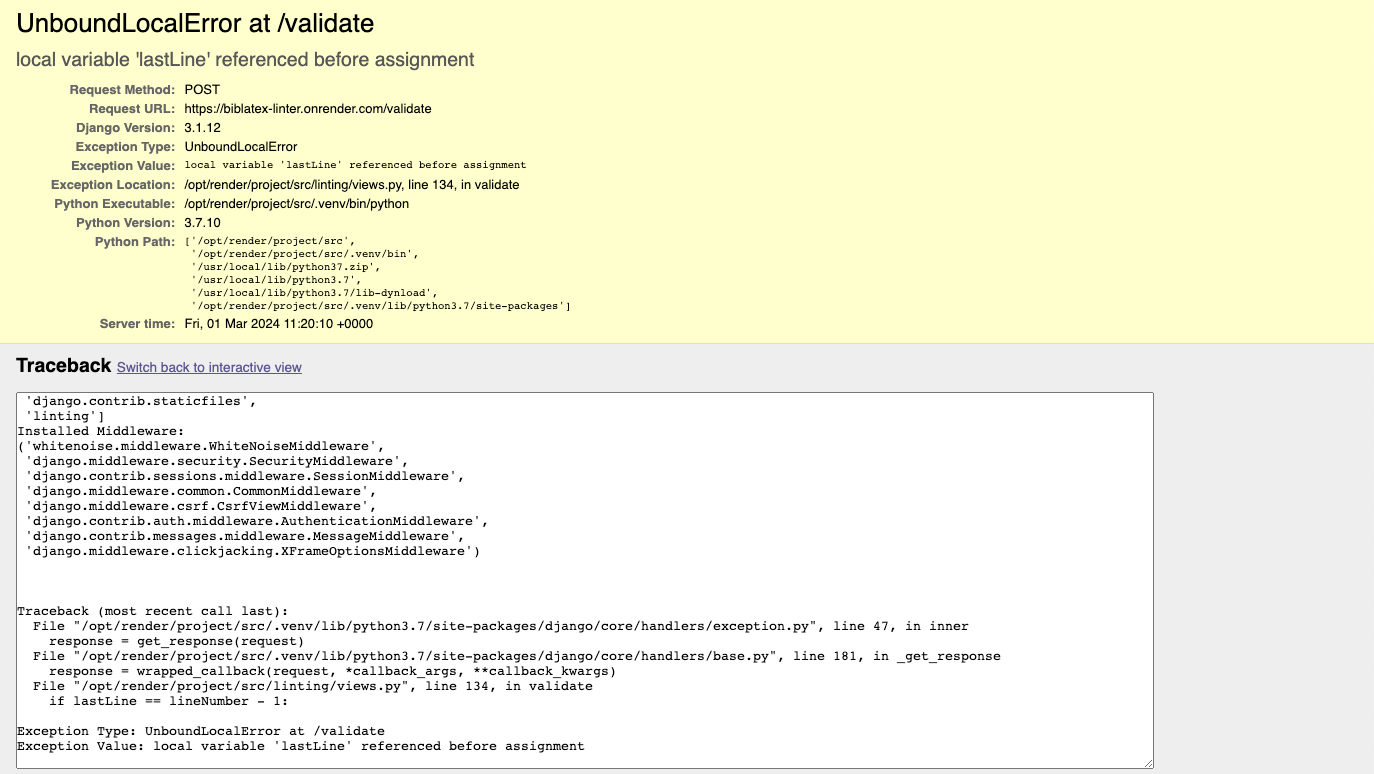
\includegraphics[width=0.7\textwidth]{./files/Pezmc-LinterError_cropped.png}
    \caption[Foutmelding BibLaTeX-linter]{Lintingerror bij het valideren van een BibLaTeX bestand.}
    \label{fig:biblatex-linter-error}
\end{figure}

Daarnaast leek de aanpak van de geschreven code ook niet optimaal te zijn op vlak van leesbaarheid en uitbreidbaarheid. Gezien dit echter wel criteria zijn waar de proof of concept aan moest voldoen, werd er besloten om deze linter niet verder te onderzoeken. Er werd wel gekeken naar de functionaliteiten die deze linter aanbood en andere zaken die handig leken om over te nemen in de eigen implementatie.


\subsection{Ruff versus de concurrentie}
\label{subsec:ruff}
Ruff\footnote{\url{https://astral.sh/ruff}} is een Python linter geschreven in Rust. Dat is ook direct waar Ruff zich onderscheid van de concurrent Python linters die gewoon in Python geschreven zijn. Rust is een programmeertaal die bekend staat om zeer snel en veilig te zijn. Dit zou dus duidelijk een goede keuze kunnen zijn voor een linter. Daarnaast is Rust ook veel lichter om te draaien op hardware dan Python, gezien Python een interpretatieve taal is en Rust een gecompileerde taal. 
Dit zou dus ook een goede keuze kunnen zijn voor een linter die in een CI-pipeline gebruikt zou worden. Ook is er slechts één versie van Rust waar steeds op verdergewerkt wordt, hierdoor wensen de developers van de Rust taal ook dat de code die in Rust geschreven wordt, steeds blijft werken. Of het nu over vijf jaar is, of over tien jaar, wat vandaag gecompileerd kan worden, zal ook binnen tien jaar nog steeds gecompileerd kunnen worden. 

Ruff zou op bepaalde taken tien tot wel honderd keer sneller kunnen zijn! Dit wekte direct al interesse op om de Rust taal eens op de proef te stellen om te zien of dit ook effectief zo was. 

\subsection{DirtyRat}
\label{subsec:dirtyrat}
DirtyRat is een JavaScript linter waar op gebotst werd tijdens het onderzoeken naar hoe een linter gemaakt kon worden. Het is een linter die zelf in JavaScript geschreven is en waarvan de stapsgewijze opbouw te vinden is in het artikel van \textcite{BorgesLate2021}. Daarnaast is ook de broncode zelf te vinden op GitHub\footnote{\url{https://github.com/JoanaBLate/dirtyrat}}. Dit was ook de reden waarom er besloten werd om JavaScript als kandidaat-programmeertaal te nemen. 

Hoewel het artikel zeer in detail gaat en het grondig onderzocht werd, werd er vastgesteld dat het toch wat te uitgebreid is voor deze proof of concept. JavaScript en andere programmeertalen zitten met veel meer complexe structureren dan een BibLaTeX bestand. Dus hoewel het interessant was om te zien hoe een linter in JavaScript gemaakt kon worden, was het dus zeker niet nodig om elke component over te nemen.

\section{Functionele en niet-functionele requirements}
Nadat de volledige reeks linters was geanalyseerd, kon een lijst van zowel functionele als niet-functionele vereisten worden opgesteld. Dankzij de promotor van deze thesis werd dat proces versneld. Een informatieve lijst werd verstrekt, waarin onder andere een opsomming van de gewenste regels stond. Aangezien de promotor uitgebreide technische kennis van het onderwerp heeft en beschouwd kan worden als de \emph{klant} bij de ontwikkeling van deze tool, werd gefocust op de uitwerking van de specifieke regels volgens zijn wensen.\newline

Een overzicht van de \textbf{functionele requirements} kan in tabel \ref{tab:functional_requirements} worden bezichtigd. Merk op dat deze lijst slechts een richtlijn is voor tijdens de effectieve uitwerking.\newline

Wat de \textbf{niet-functionele} requirements betreft:
\begin{itemize}
    \item Er wordt gewenst dat de linter gebruikt kan worden vanuit de \textbf{CLI} zodat deze in pipelines gebruikt kan worden.
    \item De linter dient \textbf{vlot} te werken, zodat de tool strict als handig beschouwd kan worden en zeker niet als iets storend.
    \item De linter dient \textbf{uitbreidbaar} te zijn eens deze proef-periode is afgelopen. Er wordt duidelijke, gestructureerde en gedocumenteerde code verwacht.
    \item Er wordt verwacht dat het \textbf{eenvoudig} te gebruiken is, begrijp hieronder dat het beschikbaar zal zijn via een pip-installatie gelijk andere Python modules.
\end{itemize}

\begin{table}[ht]
    \centering
    \begin{tabular}{p{2.5cm} p{13cm}}
        \toprule
        \textbf{Prioriteit} & \textbf{Requirement Beschrijving} \\
        \midrule
        \textbf{Musts} & 
          - Elk item moet een sleutel hebben. \\
        & - Elke BibLaTeX-sleutel moet uniek zijn. \\
        & - Alle vereiste velden moeten aanwezig en niet leeg zijn. \\
        & - Auteurnamen moeten in het juiste formaat zijn. \\
        & - Data moeten in het formaat `YYYY-MM-DD` zijn. \\
        & - Speciale tekens te vervangen door hun LaTeX-commando's. \\
        & - Paginabereiken moeten een "em-dash" gebruiken, d.w.z. `--`. \\
        & - article - Vereist: author, title, journaltitle, date. \\
        & - book - Vereist: author|editor, title, date, publisher. \\
        & - inbook - Vereist: author|editor, title, booktitle, date, publisher. \\
        & - dataset - Vereist: author|editor, title, date, url, urldate. \\
        & - manual - Vereist: author|editor, title, date. \\
        & - misc (software) - Vereist: author|editor, title, date. \\
        & - online - Vereist: author|editor, title, date, url, urldate. \\
        & - inproceedings (conference) - Vereist: author, title, booktitle, date. \\
        & - report (techreport) - Vereist: author, title, date, type, institution. \\
        & - thesis (mastersthesis, phdthesis) - Vereist: author, title, date, type, institution. \\
        \midrule
        \textbf{Shoulds} 
        & - Geef de voorkeur aan "date" boven "year" en/of "month". \\
        & - Aanbevolen velden \texttt{$(`WARN\_FIELDS`)$} moeten aanwezig en niet leeg zijn. \\
        & - article - Aanbevolen: doi, volume, number, pages. \\
        & - book - Aanbevolen: isbn. \\
        & - inbook - Aanbevolen: isbn|doi, pages. \\
        & - manual - Aanbevolen: organization|publisher, isbn|doi|url. \\
        & - inproceedings - Aanbevolen: editor, eventtitle, isbn|doi|url. \\
        & - report - Aanbevolen: doi|url. \\
        & - thesis - Aanbevolen: url. \\
        \midrule
        \textbf{Coulds} & 
          - BibLaTeX-keys moeten overeenkomen met de naam van de auteur. \\
        & - Geef de voorkeur aan originele types, niet aan aliassen. \\
        & - Verwijder tekstmarkering van URL. \\
        & - Vermijd het citeren van tertiaire bronnen. \\
        & - Citeer geen startpagina van een website. \\
        & - Geef de voorkeur aan "journaltitle" boven "journal". \\
        & - Geef de voorkeur aan "institution" boven "school". \\
        \bottomrule
    \end{tabular}
    \caption{Geprioriteerde Functionele Vereisten met behulp van de MoSCoW-methode}
    \label{tab:functional_requirements}
    \end{table}


\section{Keuze van de programmeertaal}
Om de gepaste programmeertaal te vinden, werden diverse kandidaat-programmeertalen overwogen. De kandidaat-programmeertalen waren: Rust, JavaScript en Python.

Door het analyseren van reeds bestaande linters en het afgaan van een hele lijst aan programmeertalen, werd er besloten om met deze drie programmeertalen te experimenteren. Om ervoor te zorgen dat de testprogramma's niet te uitgebreid werden en zowel gelijk als eerlijk konden worden vergeleken, zouden er slechts twee functionaliteiten worden uitgewerkt. Deze twee functionaliteiten waren: detecteren van duplicaten en detecteren of alle required fields aanwezig waren. Om dit onderzoek niet nodeloos lang te maken, werd er besloten om de broncode van deze programma's niet op te nemen in dit document. De broncode is echter wel te vinden op GitHub voor zowel de kleine poc's\footnote{\url{https://github.com/MrClassicT/bibLaTeX-linter-pocs}} als voor het uiteindelijk resultaat\footnote{\url{https://github.com/MrClassicT/bibla}}.

Het test .bib bestand dat gebruik werd, zag er als volgt uit:

\inputminted[samepage, breaklines]{bibtex} % bibtex taal wordt hier gebruikt omdat dit het dichtste aansluit bij bibLaTeX van de beschikbare opties.
{./files/test.bib} % Het test bestand van de proof of concept linters in de 3 programmeertalen.

\subsection{JavaScript}
JavaScript staat vooral gekend vanwege vanwege het gebruik binnen web applicaties. Het is echter wel een programmeertaal die zeer toegankelijk en gekend is onder de meeste developers. Dit was ook de eerste programmeertaal waarin een testversie werd opgesteld, deze werd dan achteraf verteld naar zowel Python als Rust om te kijken welke van de drie talen het meest geschikt was voor deze case. 

De JavaScript versie was van een persoonlijk perspectief de beste om mee te beginnen gezien dit de meest vertrouwde taal was. Direct kan er al opgemerkt worden dat er gebruik gemaakt werd van modules, dit was noodzakelijk om de linter overzichtelijk, uitbreidbaar en onderhoudbaar te maken. Moest alles in éénzelfde bestand zitten, zou het veel te groot en onoverzichtelijk worden.

\begin{minted}{javascript}
// Import submodules
const { exit } = require('process');
const { readFromFile } = require('./helper/readFromFileAsync.js');
const { checkForMissingFields } = require('./checks/missingfields.js');
const { checkForDuplicates } = require('./checks/duplicates.js');
const { entryPattern } = require('./components/regex.js');
const { toFileUrl } = require('./helper/getFileUrl.js')
\end{minted}

Als eerste wordt er een bestand ingelezen. Eens dat gebeurt is, dient er een onderscheid gemaakt te worden tussen alle verschillende bronnen binnen dit bestand. De bronnen in dit bestand, worden ook wel \'entries\' genoemd. Dit werd op de volgende manier gedaan:
\begin{minted}{javascript}
 // Extract all entries
 const entries = [...fileContent.matchAll(entryPattern)].map(match => ({
        type: match[1],
        citationName: match[2].trim(),
        content: match[3],
        position: match.index
    }));
\end{minted}
Op deze wijze werd niet alleen een \'entry\' ontdekt, maar werd ook meteen onderscheid gemaakt tussen de bronsoort, de sleutel, de inhoud en de positie van waar deze voorkomt in het bestand. Om dit te doen, werd er gebruik gemaakt van een reguliere expressie. Met een reguliere expressie is het mogelijk om patronen binnen teksten te vinden. Gezien de structurele vorm van een \.bib bestand, is het mogelijk om reguliere expressies op een eenvoudige manier te benutten om zo een krachtige analyse uit te voeren op de input.

In detail zal er niet ingegaan worden op hoe deze reguliere expressies werken, maar de twee reguliere expressies die nodig waren binnen deze mini-poc waren de volgende:
\begin{minted}{javascript}
// Extract each entry from the .bib file.
const entryPattern = /@(\w+)\{([^,]+),\s*(.*?)\},\s*\}/sg;
// Extract each field from the entry.
const fieldPattern = /(\w+)\s*=\s*(?:\{(.*?)\}|(\S+))/sg;
\end{minted}

De eerste zorgt ervoor dat elke bron van elkaar onderscheden kan worden. De tweede gaat dan weer van toepassing zijn op een iets lager niveau. Daarmee kan er binnen een bron gekeken worden naar de individuele velden data die ervan bijgehouden worden, of juist om te kijken naar welke velden er missen bijvoorbeeld.

Om te kijken welke velden er missen, werd volgende methode gebruikt:

\begin{minted}{javascript}
function checkForMissingFields(entry) {

    let fields = {};

    while ((fieldMatch = fieldPattern.exec(entry.content)) !== null) {
        fields[fieldMatch[1]] = fieldMatch[2] || fieldMatch[3];
    }

    let missingFields = [];
    if (entryRequirements[entry.type]) {
        entryRequirements[entry.type].required.forEach(field => {
            if (!fields[field]) {
                missingFields.push(field);
            }
        });
}

return missingFields;
}
\end{minted}
Hier wordt er een lijst gebruikt van velden die binnen de entry voor dienen te komen. Indien er gemerkt wordt dat er een bepaald veld niet in voorkomt, wordt de naam van het ontbrekende veld toegevoegd aan een lijst die teruggegeven wordt eens alles gecontroleerd is. Deze lijst wordt dan getoond aan de user.

Vóór het onderzoek naar ontbrekende velden wordt eerst gecontroleerd op eventuele duplicate entries. Ook wordt onderzocht of er mogelijk entries zijn die licht verschillen maar toch dezelfde verwijzingssleutel bevatten. Gezien het feit dat een duplicaat sleutel niet is toegestaan, wordt deze controle als eerste uitgevoerd.

\begin{minipage}{\pdfpagewidth}
Deze controle werd als volgt geïmplementeerd:

\begin{minted}{javascript}
function checkForDuplicates(entries) {
    const citationNames = entries.map(entry => entry.citationName);
    const duplicates = citationNames.filter((citationName, index, self) => 
    self.indexOf(citationName) !== index 
    && self.lastIndexOf(citationName) === index
    );

    if (duplicates.length > 0) {
        const plural = duplicates.length > 1;
        console.error(`Caution: ${plural ? "" : "A "}duplicate key
        ${plural ? "s" : ""} ${duplicates} ha${plural ? "ve" : "s"} 
        been found!`);
        exit(1);
}
}
\end{minted}
\end{minipage}
In deze controle valt op dat er een gebrek aan consistentie is in de manier waarop informatie aan de gebruiker wordt gepresenteerd. In tegenstelling tot de andere controle, waarbij dit pas achteraf gebeurde, gebeurt dit hier onmiddellijk zodra we het detecteren. Dit kan worden toegeschreven aan het feit dat dit een testversie is, ontworpen om een eerste indruk te krijgen. Bovendien zou een directe presentatie van de informatie mogelijk efficiënter kunnen zijn dan wanneer deze eerst wordt teruggestuurd naar een hoger niveau in het programma.

\subsection{Python}
\label{subsec:python}
Gezien het grote aanbod aan linters die in Python geschreven zijn en de ruime gekendheid ervan, werd er besloten om ook Python een kans te geven. Omdat de Python-kennis wat afgezwakt was, werd er beroep gedaan op de krachten van AI. De linter poc geschreven in JavaScript werd aan ChatGPT versie 4 gegeven en stapsgewijs werd er gevraagd om deze code om te vormen naar een werkend Python alternatief. Op enkele uren tijd werd erin geslaagd om een eerste versie werkende te krijgen. Het was zeer knap om te zien hoe goed ChatGPT de Python taal effectief kent. Ook de reguliere expressies die gebruikt werden, hebben op een bepaald moment in de handen van ChatGPT of zelfs github-copilot gezeten. AI-tools zijn zeer handig om complexe zaken enerzijds te verduidelijken als anderzijds erbij te assisteren om suggesties te doen van hoe een bepaald probleem aangepakt kan worden. De kracht van AI was dus hier zeker merkbaar en werd ten zeerste geappreciëerd.
\pagebreak
\begin{minted}{python3}
    entries = [match.groups() for match in entry_pattern.finditer(file_content)]
    formatted_entries = [{
        'type': entry[0],
        'citationName': entry[1].strip(),
        'content': entry[2],
        'position': match.start()
    } for match, entry in zip(entry_pattern.finditer(file_content), entries)]

\end{minted}

Als deze pythoncode vergeleken wordt met de javascript-code, kan er direct opgemerkt worden dat er gelijkaardige logica achter zit. Dit is uiteindelijk ook het geval want de javascript-code is simpelweg vertaald naar python code.

De twee functionaliteiten werden op een gelijke wijze vertaald en geïmplementeerd in de kleine python poc.

\begin{minted}{python3}
def check_for_missing_fields(entry):
    fields = {}
    for match in field_pattern.finditer(entry['content']):
        key, value1, value2 = match.groups()
        fields[key] = value1 or value2

    missing_fields = []
    if entry['type'] in entry_requirements:
        for field in entry_requirements[entry['type']]['required']:
            if field not in fields:
                missing_fields.append(field)

    return missing_fields

def check_for_duplicates(entries):
    citation_names = [entry['citationName'] for entry in entries]
    duplicates = {name for name in citation_names if citation_names.count(name) > 1}
    if duplicates:
        plural = len(duplicates) > 1
        print(f'Caution: {"A duplicate key" if not plural else "Duplicate keys"} {"has" if not plural else "have"} been found: {", ".join(duplicates)}!')
        exit(1)
\end{minted}

Nadelen zijn er natuurlijk ook aan het vertalen van bestaande code naar een andere programmeertaal met behulp van AI. Zo zullen fouten die in de ene taal bestaan, hoogstwaarschijnlijk ook gewoon mee vertaald worden. Dit was bijvoorbeeld het geval wat de reguliere expressie betrefde. Bij een eerste iteratie van deze poc, werkte één van de twee controles niet. Dit bleek achteraf te komen doordat de reguliere expressie iets te gevoelig was aan de hoeveelheid witruimte die er was. Gelukkig kon deze fout relatief snel achterhaald en opgelost worden.

Ook is het interessant om te weten dat bij deze poc het programma minder modulair was. Dit kwam door een kennisbarrière waarbij niet gekend was hoe modules echt goed werken in Python. Echter was dit geen dramatisch probleem gezien het maar een kleine poc was en de zekerheid er was dat dit met wat grondiger onderzoek op een later tijdstip opgelost zou kunnen worden.

De eerste signalen dat een goede syntax-kennis niet onbelangrijk is, doken hier al op.

\subsection{Rust}
Hoewel Rust een grote kans leek te maken om de programmeertaal te worden waarin de linter geschreven zou worden, werd er dan ook vol enthousiasme aan begonnen. Snelheid is niet de enige belangrijke factor. Ook kennis is van groot belang zoals al gemerkt werd bij de python poc. Een taal kan nog zo snel zijn, als er niemand is die er mee kan werken, dan is het nutteloos. Rust is een taal die nog niet zo lang (sinds 2015) bestaat en waar nog niet zoveel mensen mee werken, ondanks dat deze al in de top 20 meest populaire programmeertalen staat in de TIOBE Index\footnote{\url{https://www.tiobe.com/tiobe-index/}}.

Zoals eerder al enkele keren vermeld werd, was de keuze van de programmeertaal van groot belang zodat er ook na deze proef verder kon gewerkt worden aan de linter. Rust heeft daarbij de minst gunstige positie. Het was dus van groot belang om te kijken of het potentiëel in snelheid merkbaar genoeg was om de keuze te maken.

Ondanks dat er wat kennis opgedaan werd over de programmeertaal zelf, was het niet mogelijk om beide functionaliteiten werkende te krijgen binnen de Rust-poc. De kennis was simpelweg nog altijd te beperkt.
Daarom werd er besloten om de enige werkende functionaliteit te testen ten opzichte van de snelste andere poc, waarbij ook daar slechts enkel die éne controle gebruikt zou worden.

De enige functionaleit die werkend gekregen was in Rust, was de controle op duplicaten. Dit voelde toch wel als een kleine teleurstelling aan, maar vestigde nog maar eens een belang van een programmeertaal te beheersen en dat enkel AI en wat ideeën niet altijd voldoende zal zijn. Dat gaf dan ook maar direct het gevoel van jobzekerheid als programmeur.

Net zoals bij de andere twee poc's, werd er een soortgelijke werkwijze gehanteerd. Eerst worden de veschillende entries van elkaar gescheiden en vervolgens worden er de controles, of in dit geval de controle, op uitgevoerd.
\begin{minted}[samepage, breaklines]{rust}
    let entry_pattern = &patterns::patterns::ENTRY_PATTERN;

    let entries: Vec<_> = entry_pattern
        .captures_iter(&file_content)
        .map(|cap| {
            let entry_type = cap[1].to_owned();
            let citation_name = cap[2].trim().to_owned();
            let content = cap[3].to_owned();
            let line_number = file_content[..cap.get(0).unwrap().start()].lines().count();
            (entry_type, citation_name, content, line_number)
        })
        .collect();

    checker::checker::check_for_duplicates(
        &entries
            .iter()
            .map(|(a, b, c, d)| (a.as_str(), b.as_str(), c.as_str(), *d))
            .collect::<Vec<_>>(),
        &file_path,
    );
\end{minted}

Iedereen die wat programmeerkennis heeft, kan zelf ook inzien dat deze code ver van optimaal is. Maar opnieuw, de kennisbarrière was eenmaal aanwezig en met een beperkte tijd, diende er compromis gemaakt te worden. Merk op dat er veel lussen gebeuren, lussen die hoogstwaarschijnlijk overbodig of toch zeker weg te werken zijn. Er werden veel transformaties gemaakt met de data waarbij het leek dat er van het éne type naar het andere gegaan werd om dan vervolgens terug naar het éne type te gaan. Duidelijk veel overbodigheden. Voorgaande code bevatte niet eens de volledige check op duplicaten, dat was slechts het begin-bestand waaruit de applicatie start. Hieronder volgt de effectieve controle. Merk ook daar op dat er twee lussen in de methode zitten. Hoewel het grotendeels is voor zaken op een mooie manier te tonen is, blijft het merkwaardig dat er geen efficiëntere manier gevonden kon worden. ChatGPT of Github Copilot konden hier beide niet beter mee helpen dan ze tot dit punt al gedaan hebben.

\begin{minted}[samepage, breaklines]{rust}
    pub fn check_for_duplicates<'a>(
        entries: &[(&'a str, &'a str, &'a str, usize)],
        file_path: &str,
    ) {
        let mut duplicates: Vec<(&str, usize)> = Vec::new();
        let mut seen: Vec<&str> = Vec::new();

        for entry in entries.iter() {
            let citation_name = entry.1;
            if seen.contains(&citation_name) {
                duplicates.push((citation_name, entry.3));
            } else {
                seen.push(citation_name);
            }
        }

        for duplicate in duplicates {
            println!("All entry names should be unique.");
            let (entry_name, zerobased_line_number) = duplicate;
            let line_number = zerobased_line_number + 1;
            println!(
                "Duplicate field found in entry '{}' at line {}",
                entry_name, line_number
            );

            println!("External file path: {}:{}", file_path, line_number);
        }
    }
\end{minted}
\pagebreak  
 
\subsection{Keuze}
Na het opstellen van kleine prototypes in elke kandidaat-programmeertaal, werd er gekeken naar de voor- en nadelen van elk,en alsook naar de uitvoeringstijden. Hierbij werd er aan het begin van elk scriptje een timer gestart in de code en werd deze op het einde van de uitvoering gestopt waarna er nog een printfunctie gebeurde om het resultaat te tonen. De resultaten worden weergegeven in bijhorende tabel \ref{tabel:uitvoeringstijden}.

\begin{table}[ht]
    \centering
    \resizebox{\textwidth}{!}{
    \begin{tabular}{c|c|c|c}
        \toprule
        \textbf{JavaScript (Node)} \small{(ms)} & \textbf{Python} \small{(ms)} & \textbf{Rust} \small{(ms)} & \textbf{Notities} \\
        \midrule
        22,635 & 1.83867 & - & \multirow{3}{24em}{Eerst 3 maal Python, vervolgens 3 maal JavaScript achter elkaar.} \\
        12,008 & 1.56621 & - & \\
        13,735 & 1.57471 & - & \\
        \hline
         & & & \textbf{Commando} \\
        \hline
        
        27,095 & 1.76967 & - & {\multirow{2}{24em}{\texttt{\colorbox{bg}{node js/linter.js testData/test.bib \&\&}\break\colorbox{bg}{python3 py/linter.py testData/test.bib}}}} \\
        10,8 & 1.44262 & - &  \\
        \hline
        9,386 & 1.23654 & - & \multirow{2}{24em}{\texttt{\colorbox{bg}{python3 py/linter.py testData/test.bib}\break\colorbox{bg}{\&\& node js/linter.js testData/test.bib}}} \\
        11,311 & 1.36937 & - & \\
        \hline
        & & & \textbf{Notities} \\
        \hline
        - & 1.27763 & 9.669958 & \\
        - & 1.141 & 7.747833 & Enkel controle op duplicaten.\\
        - & 1.17904 & 8.652 &  \\
        \bottomrule
    \end{tabular}
    }
    \caption[Uitvoeringstijdentabel]{Tabel met de uitvoeringstijden van elke poc (in milliseconden).}
    \label{tabel:uitvoeringstijden}
    \end{table}

De linters werden allemaal op eenzelfde bestand gebruikt. Hierbij werd er eerst driemaal het Python commando achter elkaar uitgevoerd en daarna driemaal de JavaScript versie. Het concept van caching, opslaan van bepaalde data in snel beschikbaar geheugen, is hier zichtbaar. De eerste keer dat er iets gebeurd, duurt het langer dan de eerstvolgende keer dat het plaatsvindt.
Opmerkelijk is hier dat de JavaScript versie tot wel 12 keer \emph{trager} is dan de Python versie.

In een poging om het caching aspect te vermijden, werd het bestand nogmaals meerdere keren gecontroleerd, maar dit keer afwisselend JavaScript en Python. Eerst werd er tweemaal JavaScript als eerste uitgevoerd en vervolgens werd hetzelfde gedaan met Python als eerste. Wat extra opmerkelijk is hier, is dat JavaScript buiten gewoon lang nam in vergelijking met vorige keren. 27 milliseconden in vergelijking met de Python versie die het in minder dan 2 milliseconden kon. Hoewel het bij de tweede poging niet veel verschil maakte, kan er opnieuw gemerkt worden dat er een vorm van caching zal plaatsvinden waarbij het voorgaande resultaat nog altijd (deels) opgeslagen bleef. Hierdoor was de JavaScript linter in staat om het bestand meer dan dubbel zo snel uit te voeren. Wat wel nog altijd meer dan vijf keer trager was dan de Python versie. Python is dus een duidelijke winnaar in vergelijking met JavaScript op vlak van snelheid. Gezien Python daarnaast ook op de \emph{eerste} plaatst staat in de TIOBE Index (mei 2024), is het veilig om ervanuit te gaan dat er genoeg mensen de taal kennen om zeker te zijn dat de linter onderhoudbaar blijft nadat dit onderzoek afgelopen is.

Tot slot rest er nog Rust. Zoals eerder vermeld werd er niet in geslaagd om beide functionaliteiten werkende te krijgen. Daarom werd er besloten om enkel de controle op duplicaten uit te voeren. De snelheid van deze uitvoeringstijd, werd dan vergeleken met die van de Python versie, gezien deze de snelste van de twee was. Hoewel het internet deed geloven dat Rust mogelijk sneller zou zijn, bleek dit bij deze test verre van de waarheid te zijn. Python was ook in vergelijking met Rust sneller. Zoals eerder aangehaald, is de implementatiewijze van groot belang en mogelijks de oorzaak van deze resultaten. Echter geeft het nog altijd een realistisch beeld van de verwachten, moest er een linter in gemaakt worden. Door het gebrek aan kennis, zou de taal nooit tot het volle potentiëel benut kunnen worden en dus zou de linter nooit zo snel kunnen werken, als dat in theorie mogelijk zou moeten zijn.

Het is in principe wel nog perfect mogelijk dat Rust zich beter schaalt naar grotere bestanden toe. Het testbestand bevatte slechts één bron, maar wat als er honderden bronnen in zouden staan? Zou Python's uitvoertijd lineair vergroten of eerder exponentieel? Zou Rust sub-lineair evolueren? Deze vragen zullen binnen dit onderzoek onbeantwoord blijven. Kwestie dat er simpelweg onvoldoende tijd is om in deze scope op te nemen.\newline
Python is dus de winnaar uit dit onderzoek en zal gebruikt worden om de rest van deze proof of concept mee uit te werken.

\section{bibl}
Bibl is een BibTeX linter die gevonden werd net voordat er effectief van start werd gegaan met het uitwerken van een eigen linter. Na een grondige analyse, bleek dat bibl een open-source linter was die zeer goed opgebouwd, modulair en efficiënt is. Bibl deed in principe aan alle criteria waaraan de proof of concept linter moest gaan voldoen, en bij deze realisatie ontstond er een nieuwe visie.

Een linter zoals bibl maken, maar dan voor BibLaTeX in plaats van BibTeX, zag er uit als het einddoel. Echter met dat er al wat achterstand was op de planning, zou een eigen linter niet even uitgebreid uitgewerkt klaargeraken. Hoewel het concept van proof of concept misschien toch bereikt zou worden, leek het voordeliger om bibl te proberen gebruiken en dit compatibel te maken met BibLaTeX.

Gezien de verschillen tussen BibTeX en BibLaTeX, was er wel nog twijfel in hoeverre dit effectief ook mogelijk was; alsook met dat bibl pybtex gebruikt als parser. Op de site van pybtex\footnote{\url{https://pybtex.org/}} valt het volgende te lezen: 

\begin{quote}\emph{Pybtex is a BibTeX-compatible bibliography processor written in Python.}\end{quote} 

Dit wilt zeggen dat pybtex verantwoordelijk is voor de data uit de bibliografie bestanden te halen. De quote zegt niet dat het enkel werkende is voor BibTeX-bestanden, maar compatibiliteit met BibLaTeX wordt nergens expliciet vermeld. Het was dus een eigen test dat moest bepalen in hoeverre dit al dan niet een probleem was.

Om dit te testen, werd er gebruik gemaakt van een BibLaTeX-document dat gedeeld werd door de promotor van deze proef. Dit document bevatte geldige bronvermeldingen, wat dus perfect was om te kijken of bibl als basis gebruikt zou kunnen worden. Bibl werd snel geïnstalleerd dankzij de package manager van Python, pip. Vervolgens werd het lint commando uitgevoerd op het geldige BibLaTeX-document en werd er gekeken naar wat bibl ervan vond. 

Bibl crashte niet en toonde een volle lijst opmerkingen; dit was positief. Er waren bestaande regels die met de manier van werken voor BibLaTeX bestanden, nooit in orde zouden komen. Gelukkig is bibl open-source en kan er met de broncode gespeeld worden. Na wat van de linting regels uit te schakelen, werd er op een punt gekomen waaruit geconcludeerd kon worden dat bibl een perfecte basis was.
\chapter{Uitwerkingsfase}
\label{ch:uitwerkingsfase}
%In deze fase gebeurde het uitdagende werk. De proof of concept werd ontwikkeld op basis van de verkregen bronnen. Een werkende versie werd opgesteld, inclusief testen om de werking te garanderen en om het eenvoudig uitbreidbaar te maken. Niettemin werd er ook documentatie geschreven, zodat alles wat er gebeurde duidelijk was voor elke vrijwilliger die een bijdrage wenste te leveren. Hoewel dit misschien al in fase 2 had mogen plaatsvinden, werd er ook een kanbanbord opgesteld om net iets meer overzicht te bewaren in de vooruitgang van de proof of concept en zodat er een duidelijk zicht was op de haalbaarheid van de MVP.

%Aan het einde van deze fase stond er dus een werkende proof of concept beschikbaar op een GitHub-repository van de auteur van dit onderzoek, Tristan Cuvelier. 
%Er werd verwacht dat deze fase wel enige tijd in beslag zou nemen gezien het verwachte resultaat en met een marge die ruim genoeg was voor problemen die opdoken tijdens het ontwikkelen van de software.

Deze fase vond iets later plaats dan initiëel verwacht, maar verliep ook vlotter dan verwacht. Dat allemaal dankzij het ontdekken van bibl. Een gepaste \emph{rebrand} naam vinden voor bibl was misschien geen prioriteit, maar er werd toch besloten er eentje te vinden. Na wat brainstormen werd de naam bibla bedacht. Waar bibl wellicht stond voor bibTeX-Linter of iets soortgelijk, zal bibla simpelweg refereren naar BibLaTeX. Gezien Biblal minder leuk klonk, werd er dus gekozen voor bibla.

Nu deze lastige zaak afgehandeld is, werd er eerst een hele rebrand uitgevoerd op de fork van bibl; bibla was geboren.
\\
\\
In het begin was het zeer lastig om eigen regels toe te voegen, dit omdat het ondanks de grondige analyse die erop plaats vond, nog altijd een \emph{vreemd} project was. Daarom werd er besloten om eerst bestaande regels te controleren en deze te vergelijken met de eigen lijst van functionele requirements.
Zo konden er enerzijds taken worden geschrapt van zaken die reeds geïmplementeerd waren en kon er een overzicht gemaakt worden van de regels die aangepast diende te worden. 

Op deze manier werd er toch al nuttige vooruitgang geboekt en schepte dit een vertrouwensband met de bestaande codebase. Eens enkele waren regels aangepast, werden er ook eigen regels opgesteld die nodig waren.
% ----
\section{bibla}
\subsection{Behouden regels}
Deze sectie bevat de regels die volledig doorgekomen zijn vanuit \texttt{bibl} en dus geen veranderingen ondergaan zijn. Wèl is het mogelijk dat hier regels bij vermeld staan waarvan er veranderingen zijn doordat het configuratiebestand veranderingen ondergaan heeft.

Zo zijn regels voor wat de \texttt{Entries} (E) betreffen: E01 (voornaam auteur mag niet worden afgekort), E02 (middennamen die al dan niet mogen worden afgekort), E03 (vermijd het gebruik van 'Et Al' in auteursveld), E04 (bestanden moeten relatief pad gebruiken), E05 (gelinkte bestanden die afwezig zijn), E06 (onjuist DOI-formaat) en E07 (onjuist ISBN-formaat) gelijk gebleven. 

De \texttt{Database} (D) regels: D00 (Alfabetische volgorde van de bronnen), D01 (Preambule is de start van het document), D02 (Mogelijke duplicaten op basis van titel) zijn ook ongewijzigd gebleven.

De \texttt{Missing} (M) regels: M00 (Geen auteurs of redacteurs), M01 (Missend verplicht veld), M02 (Missend optioneel veld) zijn ook ongewijzigd gebleven wat de code betreft. Echter is hier wel de configuratie grondig aangepakt geweest voor M01 en M02, gezien HOGENT\footnote{\url{www.hogent.be}} zelf eigen voorkeuren heeft over welke bibliografische gegevens van een bron bijgehouden dienen te worden. Ook voor de \texttt{Unrecognized} (U) regels, zijn er enkel wijzigingen gebeurt in de configuratie. 

De \texttt{Unrecognized} (U) regels zijn ook totaal onaangepast gebleven. Hetzelfde kan gezegd worden voor de \texttt{Textual} (T) regels; opnieuw met uitzondering voor T01 (aantal spaties die als indentatie gebruikt dienen te worden), waar de configuratie van werd aangepast; uiteraard met uitzondering voor regel T00 (enkel ASCII karakters) die weggehaald werd gezien deze niet meer relevant is.

\subsection{Aangepaste regels}
\paragraph{E00 - Sleutelformaat}
\label{rule:E00}
Eén van de regels die aangepast diende te worden, was regel E00. Deze regel controleert het formaat van entry keys. Dit is vooral belangrijk om de consistentie te garanderen en om ervoor te zorgen dat er niet plots door inconsistenties een verwijzing niet gevonden kan worden. De regel ziet er als volgt uit:

\begin{minted}[autogobble, breaklines, linenos]{python3}
@register_entry_rule('E00', 'Keys of published works should have format `AuthorYEARa`')
def key_format(key, entry, database):
    """Raise a linter warning when entry key is not of format `AuthorYEARa`.

    E.g. an entry with values
    ```
    author = {Arthur B Cummings and David Eftekhary and Frank G House},
    date   = {2003-02-02}
    ```
    should have key `Cummings2003`.
    If another entry with the same year and main author is present,
    their keys should have formats `Cummings2003a` and `Cummings2003b`.
    This rule only applies when `date` and at least one author are set.

    :param key: The key of the current bibliography entry
    :param entry: The current bibliography entry
    :param database: All bibliography entries
    :return: True if the current entry's key has the specified format or
    year or author are not specified, False otherwise.
    """
    if 'date' not in entry.fields or len(entry.persons.get('author', [])) == 0:
        return True
    try:
        author = entry.persons['author'][0]
    except KeyError:
        try:
            author = entry.persons['editor'][0]
        except KeyError:
            return True
    names = author.rich_prelast_names + [name for last_name in author.rich_last_names for name in last_name.split('-')]
    date = entry.fields['date']
    year = re.search(r'\d{4}', date).group()

    # Check for 'EtAl' in the key when there are more than 3 authors
    if len(entry.persons.get('author', [])) >= 3 and 'EtAl' in key.lower():
        correct_key_unicode = names[0] + 'EtAl' + year
    # Check for two names in the key when there are exactly 2 authors
    elif len(entry.persons.get('author', [])) == 2:
        correct_key_unicode = "".join([str(name) for name in names[:2]]) + year
    else:
        correct_key_unicode = "".join([str(name) for name in names]) + year

    correct_key_ascii = unidecode(str(correct_key_unicode))
    regex = re.compile(correct_key_ascii + r'[a-zA-Z]?')
    return bool(regex.match(key))
\end{minted}
\captionof{listing}[bibla: E00 - Correct \texttt{key} formaat]{bibla: E00 - Sleutels moeten het juiste formaat hebben. De aangepaste versie. Aanpassingen waren nodig vanwege het gebruik van het 'date' field in plaats van het voormalige 'year' field. \label{lst:bibla_AR_E00}}


Gezien bij bibTeX de datum opgesplitst werd in \texttt{year}, \texttt{month} en \texttt{day} velden, diende deze regel aangepast te worden om rekening te houden met het \texttt{date} veld in de plaats (zie regel 21). Alsook diende er een \acrfull{REGEX} toegevoegd te worden om rekening te houden met het veranderde datum formaat. Het jaar moest immers uit het date field gehaald worden gezien het geen veld op zich meer was, zie regel 32. Daarnaast werd er ook een controle toegevoegd voor wanneer er geen author aanwezig was en bijvoorbeeld enkel een editor. \texttt{bibl} hield er namelijk geen rekening mee dat er enkel editors aanwezig zouden kunnen zijn in een bepaalde bron. Bij het uitwerken van deze proef is er een bron in de bibliografie geraakt waarbij dit het geval was. Dit had als gevolg dat de linter crashte bij het linten van dit bibliografisch bestand.
Daarnaast moest het ook mogelijk zijn om achternamen van twee auteurs te gebruiken in een sleutel of zelf 'EtAl' indien het er drie of meer waren. Ook hiervoor werden er enkele controles op punt gezet om hier rekening mee te houden, zie code-regel 35 tot en met 41.

\paragraph{E08 - \texttt{pages} veld formaat}
Deze test leek niet te werken vanwege het veld waarop gecontroleerd werd. Er werd naar het \texttt{page} veld gezocht, maar het veld waar effectief naar gezocht diende te worden staat gekend als \texttt{pages} in BibLaTeX. Uiteindelijk werd deze regel een samenvoeging van de voormalige regel E08 (pagina formaat moet xx--yy zijn) en E09 (eindpagina dient groter te zijn dan de startpagina) uit \texttt{bibl}.

\paragraph{E09 - Correct \texttt{date} formaat}
Zoals bij regel E00 (\ref{rule:E00}) reeds besproken was, is het gebruik van data wat veranderd. Nu er geen apart veld meer gebruikt wordt voor \texttt{year}, \texttt{month} en \texttt{day}, dient er een extra controle te gebeuren om te zien of de datum van een bron wel goed geformatteerd is. Waar de originele regel van bibl enkel keek of de maand weldegelijk in 'MMM' formaat was, dient er nu gekeken te worden dat het formaat gelijk is aan 'YYYY-MM-DD'. Deze regel vervangt de in \texttt{bibl} gekende regel E10 waarbij de maand in \texttt{mmm}-formaat diende te zijn.

\begin{minted}[autogobble, breaklines, linenos]{python3}
    if 'date' not in entry.fields:
        return True
    date = entry.fields['date']
    regex = re.compile(r'^(\d{4})-(\d{2})-(\d{2})$')
    match = regex.match(date)
    if not match:
        regex = re.compile(r'^(\d{4})-(\d{2})$')
        match = regex.match(date)
        if not match:
            regex = re.compile(r'^(\d{4})$')
            match = regex.match(date)
            if not match:
                return False
            return True
        year, month = map(int, match.groups())
        if not (1 <= month <= 12):
            return False
        return True
    year, month, day = map(int, match.groups())
    if not (1 <= month <= 12):
        return False
    if not (1 <= day <= 31):
        return False
    return True
\end{minted}
\captionof{listing}[bibla: E09 - Correct \texttt{date} formaat]{bibla: E09 - Correct \texttt{date} formaat. Deze regel werd gewijzigd gezien het vermelden van data gewijzigd is. Gebruikt nu \texttt{date} veld in plaats van de \texttt{year}, \texttt{month} en \texttt{day} velden. Dit is de logica. \label{lst:bibla_AR_E09}}

Ook hier is er op meerdere plaatsen weer een \acrfull{REGEX} te zien. \acrshort{REGEX} zijn krachtig voor het controleren van bepaalde vaste tekstuele structuren. In deze use case zijn ze bijvoorbeeld zeer handig om het \texttt{date} veld op te splitsen. Bij de eerste check, zie regel 4, kan al direct gezien worden of het een '4-2-2' formaat is, of toch eerder een '2-2-4' formaat. Gezien zowel de maand als dag met twee getallen voorgesteld worden, is het belangrijk om hier een minimale vorm van controle op uit te voeren. Zo kan het maandnummer nooit groter zijn dan 12 en zijn er maar maximaal 31 dagen tijdens de langste dagen. Hoewel dit niet elke fout kan tegengaan, is het wel handig om deze minimale controles uit te voeren om zoveel mogelijk garantie te bieden dat er geen grove fouten optreden op vlak van consistentie in de \texttt{date} velden. Regels 6 tot en met 18 voeren de controle uit om te zien wanneer de dag en/of maand moest ontbreken, om te zien dat ook dan het formaat zo goed mogelijk gerespecteerd wordt.


\subsection{Nieuwe regels}
\paragraph{E1O - Gebruik van Velden}
\label{rule:E10-field-preferences}
Zoals bij de aanpassingen gemerkt kon worden, was het gebruik van andere velden toch wel een aanpassing. Echter is het niet te voorkomen dat er nooit nog de \emph{oudere} velden gebruikt worden om data in op te slaan. Om de gebruikers zo goed mogelijk te ondersteunen, werd er een regel opgesteld waardoor de voorkeursvelden en hun aliassen konden gecontroleerd worden. De regel gaat op zoek naar oudere varianten/naamgevingen en suggereerd dan het nieuwere veld aan in de plaats. 

Er kan terug gedacht worden aan de \texttt{year}, \texttt{month} en \texttt{day} velden, waarvoor nu de voorkeur gaat om \texttt{date} te gebruiken.

De regel die dit controleert zag er als volgt uit:

\begin{minted}[autogobble, breaklines, linenos]{python3}
        def register_variant_rule(entry_type, field, variant):
        rule_id = 'E10{}{}'.format(entry_type.capitalize(), field.capitalize())
        message = "Entry type {} - use {} instead of {}!".format(entry_type, variant, field)
        
        @register_entry_rule(rule_id, message)
        def check_variant_field(key, entry, database, entry_type=entry_type, field=field, variant=variant):
        """Raise a linter warning when a specific field is used instead of its variant.
        
        This function checks if the variant field is required and if the specific field is present.
        If these conditions are met, it suggests to use the variant field instead of the specific field.
        
        :param key: The key of the current bibliography entry
        :param entry: The current bibliography entry
        :param database: All bibliography entries
        :param entry_type: Anchor variable to pass the local variable `entry_type` from outer scope
        :param field: The field that is being checked
        :param variant: The field that should be used instead
        :return: False if the specific field is used instead of its variant, True otherwise
        """
        if entry.type == entry_type and field in entry.fields:
            return False
        else:
            return True
\end{minted}
\captionof{listing}[bibla: E10 - Gebruik aanbevolen velden]{bibla: Nieuwe Regel | E10 - Gebruik aanbevolen velden in plaats van gelijkaardigen. \label{lst:bibla_NR_E10}}

Net zoals bij de originele regels van bibl, wordt er ook bij de nieuwe aandacht besteed aan een correcte documentatie van de code. Het is namelijk dankzij deze zorgvuldige documentatie dat gebruikers en bijdragers (Engels: Contributors) in staat zijn om te begrijpen wat er gaande is en hun bijdrage te leveren zonder onnodig tijd te moeten verspillen aan het ontcijferen van bestaande code.
    
Bij deze regel kan ook duidelijk gezien worden dat er inspiratie gehaald werd bij een reeds bestaande regels die op een zeer gelijkaardige manier te werk gaan. De regels M01 en M02 zijn een grote inspiratie geweest. De regels zijn simpel maar zeer efficiënt. Er wordt een lijst \emph{dictionary} bijgehouden waarbij de 'oude' velden als \emph{key} dienen en de 'nieuwe' als \emph{value}.
% ---

\paragraph{E11 - Gebruik van Aliassen}
\label{rule:E11-alias-preferences}
Binnen BibLaTeX zijn er vaak vele varianten beschikbaar voor bepaalde types bronnen, deze varianten vereisen dan dezelfde fields als het \emph{originele} type. Om consistentie te garanderen, gaat de voorkeur uit om altijd het \emph{originele} type te gebruiken in plaats van één van de aliassen. Deze methode werd op een gelijkaardige manier uitgewerkt als E10, M01 en M02 waar er gekeken wordt naar de bepaalde velden die al dan niet gebruikt worden. Het enige verschil is dat er hier niet naar de velden gekeken worden van een \emph{entry} maar wel naar het type van de \emph{entry}.
%---
\paragraph{E12 - Geen startpagina's in \texttt{URL} veld}
Startpagina's zijn te algemeen en verwijzen meestal niet naar een geldige bron, daarom is het van groot belang dat de correcte URL opgeslagen wordt, zodat ook na het raadplegen van een bron voor de eerste keer, dezelfde bron eenvoudig achterhaald kan worden. Ook voor in de bibliografie is het van groot belang dat dit correct opgeslagen wordt. Deze regel wordt nagekeken door opnieuw gebruik te maken van \acrshort{REGEX}. De code binnen deze regel ziet er als volgt uit:
\begin{minted}[autogobble, breaklines, linenos]{python3}
    if 'url' not in entry.fields:
        return True
    url = entry.fields['url']
    regex = re.compile(r'^(https?://)?[^/]+/?$')
    if regex.match(url):
        return False
    return True
\end{minted}
\captionof{listing}[bibla: E12 - Geen startpagina's gebruiken]{bibla: Nieuwe Regel | E12 - Gebruik geen startpagina's in het \texttt{URL} veld, logica. \label{lst:bibla_NR_E12}}

Op regel 4, in de \acrshort{REGEX} kan er gezien worden dat er gekeken wordt naar hoe een typische URL eruit kan zien, rekeninghoudende met al dan niet optionele componenten uit een URL.
% ---

\paragraph{E13 - Enkel kritische pad in \texttt{URL} veld}
% TODO - Hier verder uitschrijven.
\begin{minted}[autogobble, linenos, breaklines]{python3}
if ('#' or '?' or '%') in url:
\end{minted}

%---
\paragraph{M03 - Speciale karakters}

Deze regel zal wellicht later van naam veranderen, gezien het niet direct onder de meest intuïtieve categorie staat (M). 'M' wordt doorgaans gebruikt voor 'Missing' of ontbrekende zaken aan te duiden. Al kan er gediscussiëerd worden of dit dan niet net toch de juiste categorie zou zijn, gezien het om een ontbrekend karakter gaat. Speciale karakters dienen namelijk vervangen te worden door het commando om ze te genereren. Het commando is doorgaans gewoon een \backslash voor het karakter plaatsen. Dit zorgt ervoor dat LaTeX het speciale karakter niet gaat zien als een commando dat het moet uitvoeren. 


\begin{minted}[autogobble, breaklines, linenos]{python3}
    @register_entry_rule('M03', 'Special characters should be replaced by the command to generate them: %, &, $, #, _, \\, ~, ^, |')
    def check_special_characters(key, entry, database):
        """Raise a linter warning when a field contains special characters that should be replaced.
        :param key: The key of the current bibliography entry
        :param entry: The current bibliography entry
        :param database: All bibliography entries
        :return: True if no field contains special characters, False otherwise.
        """
        special_chars = ['%', '&', '$', '#', '_', '\\', '~', '^', '|']
    
        for field in entry.fields.values():
            if any(char in field for char in special_chars):
                for char in special_chars:
                    if char in field and field[field.index(char) - 1] != '\\':
                        return False
        return True
\end{minted}
\captionof{listing}[bibla: M03 - Speciale karakters dienen gegenereerd te worden]{bibla: Nieuwe Regel | M03 - Speciale karakters dienen met commando gegenereerd te worden. \label{lst:bibla_NR_M03}}

Hoewel deze versie gebruikt wordt in versie 2.0.5 van bibla, zit hier nog een kleine \emph{bug} in. Het is namelijk zo dat deze regel elk veld zal controleren op speciale karakters. Hoewel dit over het algemeen goed is, gooit het hierdoor ook foutieve waarschuwingen op het \texttt{url} veld.


%----

\subsection{Diverse aanpassingen}
Ondanks dat \texttt{bibl} een uitstekende start was voor deze \acrlong{POC}, waren er nog een paar zaken ter verbetering vatbaar. Foutafhandelingen waren hier een deel van. Ze dienen niet direct als een regel gezien te worden, maar ze kunnen wel voorkomen door regels die overtreden worden. Zo was bijvoorbeeld het bevatten van duplicate entry keys een reden waardoor de applicatie het soms begaf. Dit werd opgelost door een 'exception handler', ook wel foutafhandelaar genoemd, toe te voegen. Hoewel dan niet het hele bestand gelind werd, vanwege de vroegtijde fout in het programma, wordt er nu tenminste wel op een minder schokkerende wijze getoond wat er mis is en gewijzigd dient te worden. Hetzelfde werd voorzien voor wanneer er gewoon lege entries waren.  

\begin{minted}[autogobble, breaklines, linenos]{python3}
try:
    bib_data = parse_file(bibliography, macros=MONTH_NAMES)
except BibliographyDataError as e:
    # Extract the key from the error message
    match = re.search(r'repeated bibliograhpy entry: (.*)', str(e))
    if match:
        duplicate_key = match.group(1)
        print(f"{bibliography} D03: Duplicate entry with key '{duplicate_key}'")
    else:
        print(f"Warning: {e}")
    return []
except pybtex.scanner.TokenRequired as e:
    print(f"E00: {e}")
    return []
except Exception as e:
    print(f"Error: {e}")
    return []
\end{minted}
\captionof{listing}[bibla: Extra foutafhandelingen]{bibla: Diverse aanpassing | Foutafhandelingen om de tool properder te laten werken. \label{lst:bibla_foutafhandelingen_voorbeeld}}

In dit codeblock, genomen uit \texttt{lint.py}, kan er gezien worden dat er aan extra foutafhandelingen gedaan wordt. De regels die hier overtreden worden, staan op dit ogenblik vast gecodeerd en zijn minder dynamisch dan doorheen de rest van de applicatie gewend is, maar ze zijn afgestemd geweest en als de testen als betrouwbaar gezien kunnen worden, zou dit kloppen met wat de oorzaak achterliggend effectief is. Dit was de meest eenvoudige en duidelijke manier om de gebruiker te laten weten wat er mis is zonder kostbare tijd te verliezen voor het verder ontwikkelen van andere delen van de applicatie.

\subsection{Configuratie}
De standaardconfiguratie van bibl was een zeer goede basis om van verder te gaan voor bibla. Maar zoals al vaker aangegeven, zijn er verschillen tussen bibTeX en bibLaTeX die ervoor zorgen dat er aanpassingen dienen te gebeuren. Op de configuratie van bibl\footnote{\url{https://gitlab.com/arnevdk/bibl/-/blob/master/bibl/bibl.yml}} zijn er zaken veranderd, maar ook extra toegevoegd. Zoals voor bijvoorbeeld regel E10 (\ref{rule:E10-field-preferences}) waar er gekeken werd naar bepaalde velden waarbij er een voorkeur is om er een synoniem van te gebruiken. Waarvan hieronder het stukje configuratie in YAML-formaat.


\begin{minted}[autogobble, breaklines, linenos]{yaml}
alternate_fields:
  # preferred: [other]
  date: [year] # Month and day will not be used alone, so when we just check for the year, that'll be fine.
  journaltitle: [journal]
  institution: [school]
\end{minted}
\captionof{listing}[bibla: Configuratie | E10 - Gebruik aanbevolen velden]{bibla: Configuratie | E10 - Gebruik aanbevolen velden in plaats van gelijkaardigen. \label{lst:bibla_AC_E10}}
   
De overige configuratie kan geraadpleegt worden op de \texttt{bibla} repository in \texttt{bibla.yml}\footnote{\url{https://github.com/MrClassicT/bibla/blob/master/bibla/bibla.yml}}, wat de algemene configuratie voor \texttt{bibla} bevat.

\subsection{Pipelines}
\texttt{bibl} werkte met GitLab, \texttt{bibla} werkt met GitHub. Het is dus niet onlogisch dat er nog enkele andere zaken aangepast dienen te worden om alles vlot te laten verlopen. Hierbij denken we vooral aan de pipelines die gebruikt worden. \texttt{bibl} bevat slechts één pipeline bestand\footnote{\url{https://gitlab.com/arnevdk/bibl/-/blob/master/.gitlab-ci.yml}}, een continuous integration. Al gebeurt er in deze pipeline ook een \emph{deploy} van een statische website die alle linterregels bevat.

Op GitHub worden pipelines gekend onder \emph{workflows}, wat reflecteert naar wat een pipeline effectief inhoudt. Gezien de \emph{workflows} iets anders zijn dan de gewone pipelines op GitLab, diende er enkele wijzigingen te gebeuren. Zo diende de pipelines te komen in een folder \texttt{.github/workflows} om herkend te worden. Hierin werd er een omgevormde CI-pipeline geplaatst, gebaseerd op de originele van \texttt{bibl}.

\paragraph{CI-pipeline}
\begin{minted}[autogobble, breaklines, linenos]{yaml}
name: CI Workflow

on:
  push:
    branches:
      - master

jobs:
  build:
    runs-on: ubuntu-latest
    strategy:
      matrix:
        python-version: ["3.12"]
    steps:
    - uses: actions/checkout@v4

    - name: Set up Python ${{ matrix.python-version }}
      uses: actions/setup-python@v4
      with:
        python-version: ${{ matrix.python-version }}

    - name: Install dependencies
      run: |
        python -m pip install --upgrade pip
        pip install git+https://${{secrets.BIBLA_GITHUB_TOKEN}}@github.com/mrclassict/bibla.git
        pip install --upgrade setuptools wheel
        pip install -e .[dev]
        pip install flake8

    - name: Static Analysis with Flake8
      run: |
        mkdir out
        flake8 --append-config .flake8 --ignore=E501 | tee out/lint_result.txt
        num_warnings=$(wc -l < out/lint_result.txt)
        echo "$num_warnings warnings!"
        echo "Generating badge..."
        anybadge -v=$num_warnings -f=out/flake8.svg -l=flake8 10=green 1000=orange 10000=red
        cat out/lint_result.txt
        if [ $num_warnings -gt 0 ]; then exit 1; fi

    - name: Upload artifacts
      uses: actions/upload-artifact@v4
      with:
        name: flake8-results
        path: |
          out/flake8.svg
          out/lint_result.txt
\end{minted}
\captionof{listing}[bibla: \acrshort{CI}-pipeline]{bibla: \acrshort{CI}-pipeline | \acrfull{CI} pipeline overzicht \label{lst:bibla_CI}}

Bij het analyseren van deze pipeline, kan er gezien worden dat er vier zaken gebeuren:
\begin{enumerate}
    \item De juiste Python-versie installeren (in dit voorbeeld 3.12)
    \item Dependencies installeren
    \item De code linten met flake8
    \item Artifacts uploaden
\end{enumerate}

Deze stappen gebeuren op een virtuele machine op de GitHub servers en ze gebeuren elke keer dat er een \emph{push} gebeurt naar de 'master' branch.
Hoewel in deze pipeline net gelijk bij \texttt{bibl} Flake8 gebruikt wordt om de code te linten, werd er ondertussen geleerd dat Ruff wellicht een interessantere optie is. Naar de toekomst toe kan het interessant zijn om hier eens naar te kijken en eventueel over te schakelen van linting-tool.


\paragraph{CD-pipeline}
Om ervoor te zorgen dat bij elke \emph{release} (of uitgave in het Nederlands) \texttt{bibla} eenvoudig en consistent naar de pakketmanager gestuurd kon worden, werd er ook een CD-pipeline voorzien. Het opzetten van deze pipeline ging dankzij de templates die GitHub voorziet in minder dan vijf minuten! Het enige dat zelf diende te gebeuren, was een API-token (een vorm van zowel identificatie en authenticatie) voorzien en de CD-pipeline-template deed de rest.

\begin{minted}[autogobble, breaklines, linenos]{yaml}
# This workflow will upload a Python Package using Twine when a release is created
# For more information see: https://docs.github.com/en/actions/automating-builds-and-tests/building-and-testing-python#publishing-to-package-registries

# This workflow uses actions that are not certified by GitHub.
# They are provided by a third-party and are governed by
# separate terms of service, privacy policy, and support
# documentation.

name: Upload Python Package

on:
  release:
    types: [published]

permissions:
  contents: read

jobs:
  deploy:

    runs-on: ubuntu-latest

    steps:
    - uses: actions/checkout@v4

    - name: Set up Python
      uses: actions/setup-python@v3
      with:
        python-version: '3.x'
    - name: Install dependencies
      run: |
        python -m pip install --upgrade pip
        pip install build
        pip install markdown

    - name: Build package
      run: python -m build

    - name: Publish package
      uses: pypa/gh-action-pypi-publish@27b31702a0e7fc50959f5ad993c78deac1bdfc29
      with:
        user: __token__
        password: ${{ secrets.PYPI_API_TOKEN }}

\end{minted}
\captionof{listing}[bibla: \acrshort{CD}-pipeline]{bibla: \acrshort{CD}-pipeline | \acrfull{CD} pipeline overzicht \label{lst:bibla_CD}}
%\input{...}
%...

%%=============================================================================
%% Conclusie
%%=============================================================================

\chapter{Conclusie}%
\label{ch:conclusie}

% TODO: Trek een duidelijke conclusie, in de vorm van een antwoord op de
% onderzoeksvra(a)g(en). Wat was jouw bijdrage aan het onderzoeksdomein en
% hoe biedt dit meerwaarde aan het vakgebied/doelgroep? 
% Reflecteer kritisch over het resultaat. In Engelse teksten wordt deze sectie
% ``Discussion'' genoemd. Had je deze uitkomst verwacht? Zijn er zaken die nog
% niet duidelijk zijn?
% Heeft het onderzoek geleid tot nieuwe vragen die uitnodigen tot verder 
%onderzoek?

% Wat zijn de requirements die in de POC zijn voldaan en welke dienen nog verricht te worden? 
% Conclusie, huidige stand, toekomst visie?

Deze bachelorproef richtte zich op het ontwikkelen van een proof of concept voor een BibLaTeX-compatibele linter, gebaseerd op de bestaande \texttt{bibl}-tool, een linter voor BibTeX. Door de keuze voor Python als programmeertaal en de solide structuur van \texttt{bibl}, is een functionele en effectieve linter gerealiseerd die BibLaTeX-bestanden kan analyseren en valideren.

Tijdens de ontwikkeling en testen van deze linter is gebleken dat de tool over het algemeen betrouwbaar en consistent is en nauwkeurige resultaten levert. Dankzij feedback van de promotor en medestudenten zijn diverse bugfixes doorgevoerd, wat heeft bijgedragen aan de verbetering van de tool en heeft geleid tot minder foutieve detecties. Hoewel er nog enkele mankementen zijn, worden deze actief gemeld via GitHub 'issues' en voortdurend aangepakt. Dit iteratieve proces zorgt ervoor dat de linter steeds verder wordt verbeterd en dat er ruimte blijft voor het toevoegen van extra functionaliteiten in de toekomst. Dit toont de doeltreffendheid van de linter en de waarde van een iteratief ontwikkelingsproces.
% ---
\section{Nog uit te werken requirements}
Naast alle uitgevoerde functionaliteiten, zijn er enkele die niet afgerond zijn. Een functionaliteit die prioriteit zou mogen krijgen, is het controleren of auteurs/redacteuren hun namen in het correcte formaat hebben geschreven. Gezien de manier waarop Pybtex deze uitleest, bleek dit complexer dan verwacht en werd deze feature daarom als out of scope beschouwd voor deze POC. Daarnaast moet er nog een methode worden gevonden om te controleren of tertiaire of illegale bronnen gebruikt worden, zodat ook deze afgeraden kunnen worden. Een andere kleinere feature die wegens tijdsgebrek niet volledig klaar is, is een online lijst van alle regels. Deze zou tijdens het uitvoeren van de pipelines aangemaakt worden en achteraf gepubliceerd worden. GitHub Pages\footnote{\url{https://pages.github.com/}} is een optie die hiervoor gebruikt zou kunnen worden.

% ---

\section{Was de proof of concept een succes?}

Er kan geconcludeerd worden dat het resultaat van dit project een groot succes is. De linter functioneert naar behoren en kan effectief worden ingezet als analysetool voor BibLaTeX-bestanden; zeker binnen de HOGENT-omgeving, aangezien de regels de voorkeuren van HOGENT\footnote{\url{www.hogent.be}} respecteren. Deze tool stelt gebruikers in staat om consistentie en validiteit in hun bronvermeldingen te waarborgen, wat essentieel is voor academische werken. Dankzij de bekendmaking van de tool door de promotor en docent aan HOGENT aan medestudenten, kon de tool al getest worden. Eén van deze medestudenten heeft een schermafbeelding voorzien waaruit de effectiviteit van \texttt{bibla} aangetoond kan worden, zie Figuur \ref{fig:bibla-is-useful}.
\\
\\
Samenvattend biedt \texttt{bibla} een meer uitgebreide en gedetailleerde set regels die beter zijn afgestemd op de eisen van BibLaTeX in vergelijking met \texttt{bibl}. De aanvullende en aangepaste regels (zie Sectie \ref{sec:bibla205}) zorgen voor een grotere nauwkeurigheid en consistentie in de verwerking van bibliografische vermeldingen. Door het volgen van deze regels kunnen gebruikers ervoor zorgen dat hun BibLaTeX-bestanden voldoen aan de huidige standaarden en best practices die voor deze use case werden opgelegd door HOGENT.

\begin{figure}[ht]
    \centering
    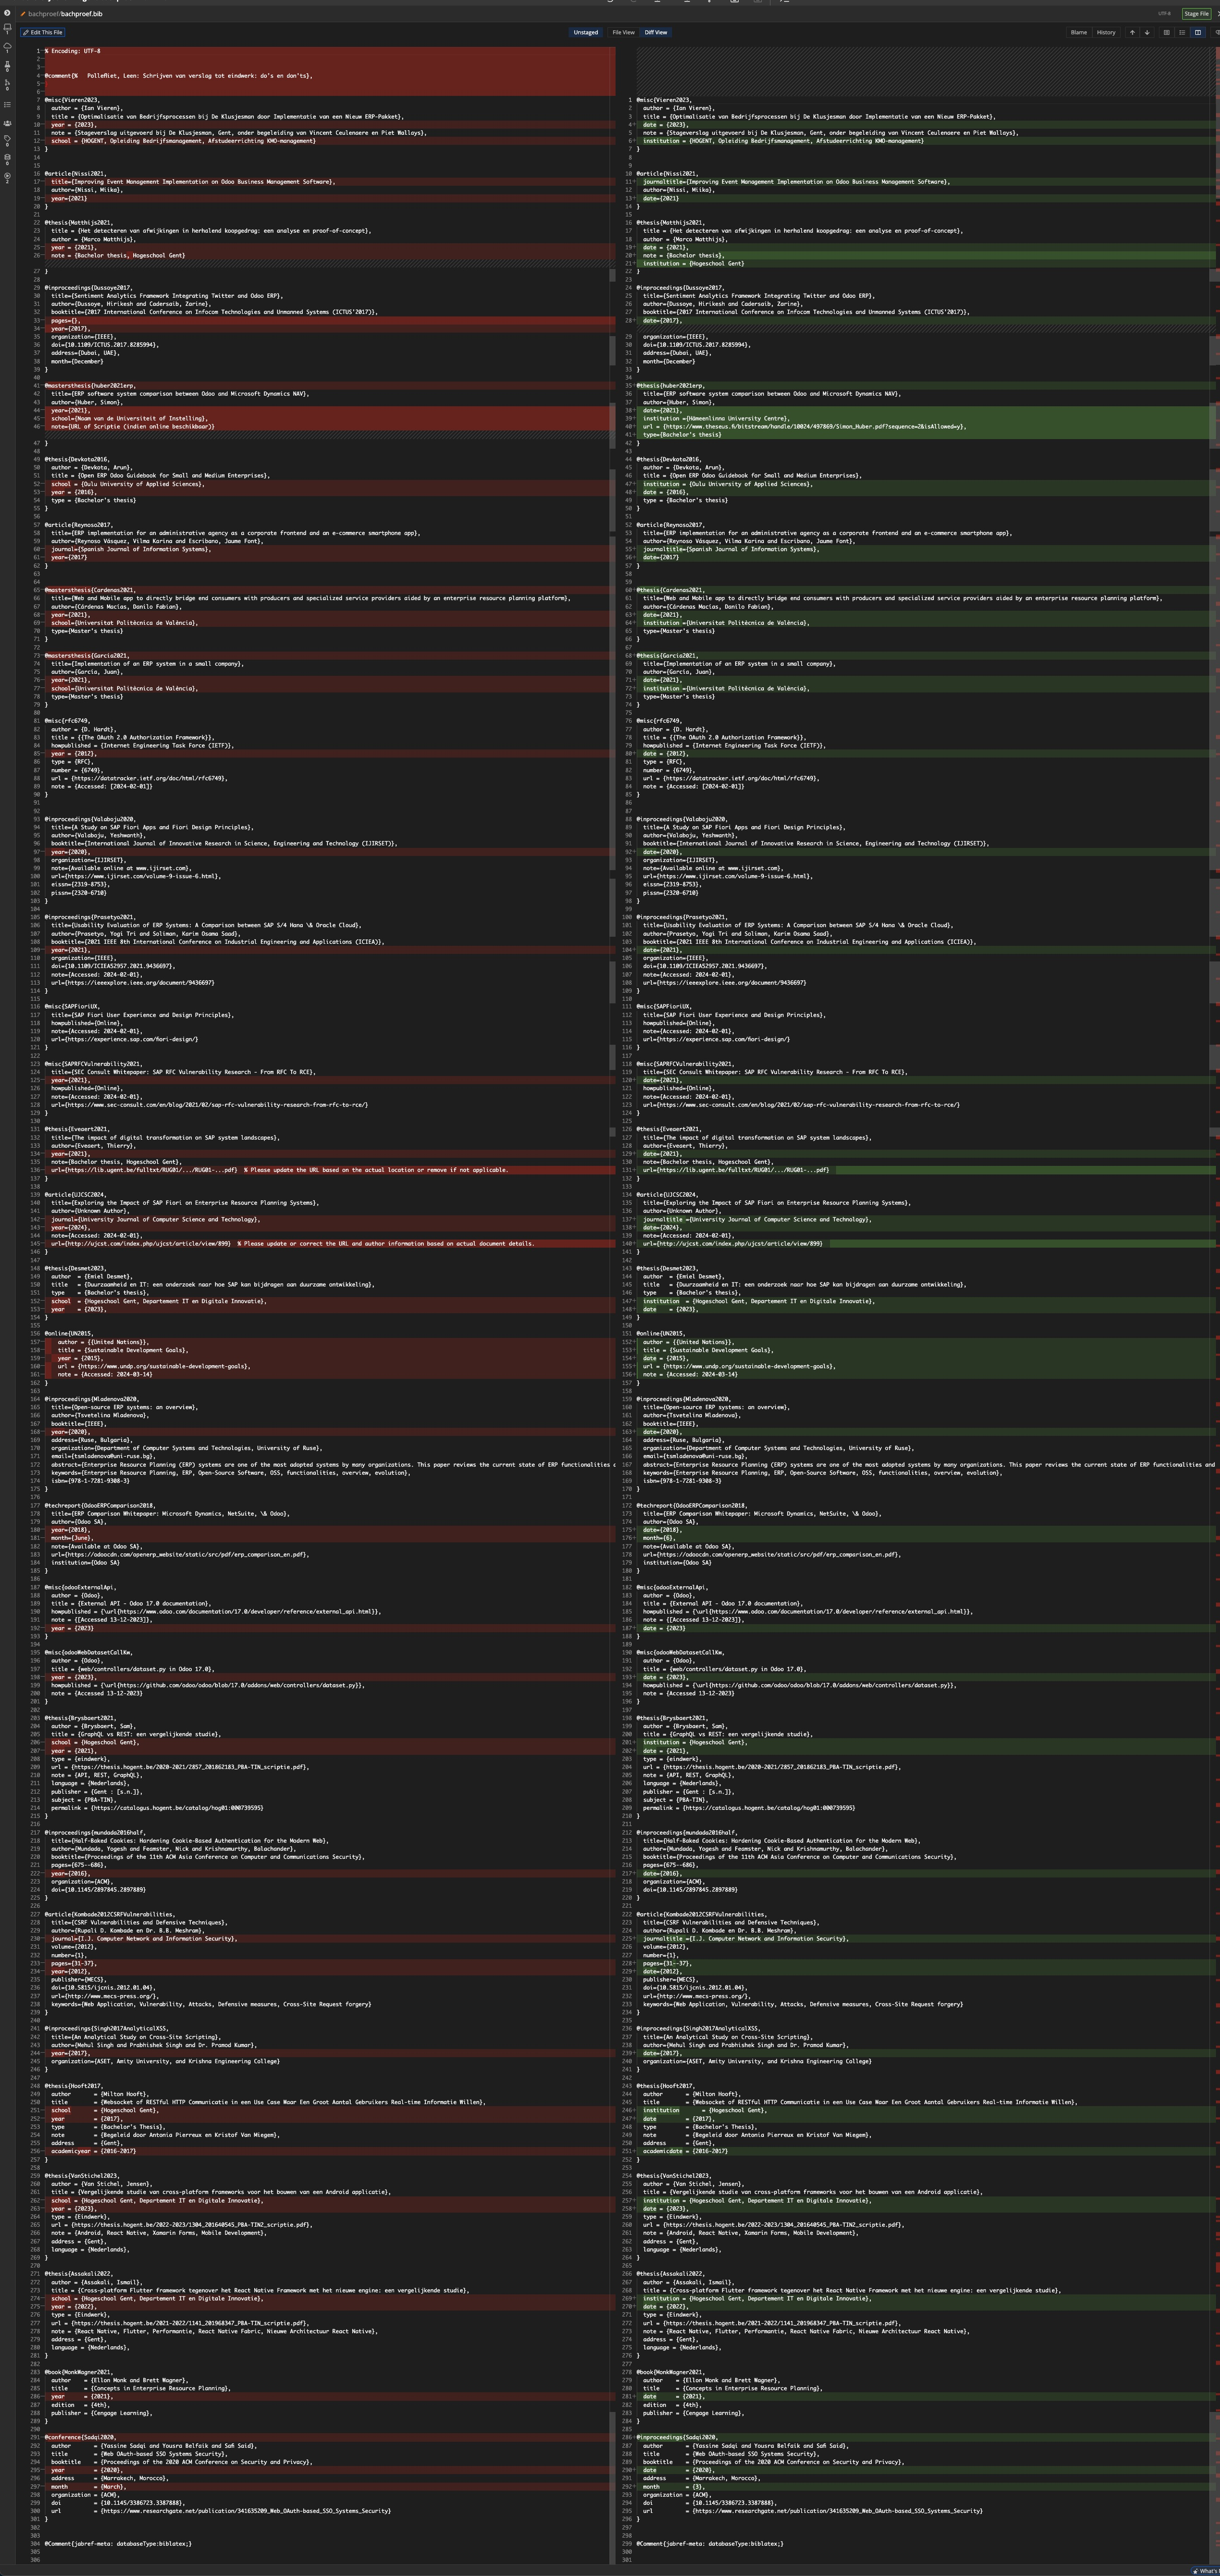
\includegraphics[width=0.7\textwidth]{./files/bibla_is_useful.jpeg}
    \caption[Effectiviteit bibla]{Deze afbeelding toont de \textbf{capaciteiten} van \textbf{bibla}. Een gebruiker heeft dit gedeeld, op de afbeelding kan het rode gezien worden als wat weggehaald werd en het groene als wat er in de plaats bijgekomen of ter vervanging is. Hoewel de afbeelding wat enigszins onduidelijk is, kunnen de aantal veranderingen die dienden te gebeuren wel waargenomen worden. Dit illustreert het \textbf{aantal fouten} waarvan docenten - \textbf{per student} - bespaard zullen worden om ze iedere keer zelf aan te moeten halen en anderzijds heeft deze gebruiker nu een correctere bibliografie.}
    \label{fig:bibla-is-useful}
\end{figure}

\section{Toekomstvisie}
Het gebruik van \texttt{bibla} als de standaard bronvermeldingsanalysetool binnen HOGENT is een veelbelovende stap. Door de implementatie van \texttt{bibla} zullen studenten en docenten profiteren van een uniforme en betrouwbare methode om BibLaTeX-bestanden te controleren. Dit zal de kwaliteit van academische werken verbeteren en de werkdruk verlagen doordat veelvoorkomende fouten automatisch worden gedetecteerd.

De ontwikkeling van \texttt{bibla} staat echter niet stil. Nieuwe features en regels zullen blijven worden toegevoegd om de functionaliteit van de linter uit te breiden. Dit omvat bijvoorbeeld het toevoegen van extra types bronvermeldingen en het verbeteren van bestaande regels om nog nauwkeuriger te zijn. Daarnaast zullen eventuele nieuwe bugs worden aangepakt en opgelost om ervoor te zorgen dat de linter zo feilloos mogelijk kan werken.

Met \texttt{bibl} als stevige fundering was het mogelijk om \texttt{bibla} te ontwikkelen. De modulaire en uitbreidbare architectuur van \texttt{bibl} heeft bijgedragen aan een soepel ontwikkelproces en biedt een solide basis voor verdere uitbreidingen. Deze fundering zorgt ervoor dat \texttt{bibla} niet alleen nu, maar ook in de toekomst een waardevol hulpmiddel zal blijven voor de academische gemeenschap van HOGENT.

\section{Aanbevelingen}

Voor toekomstige ontwikkelaars en gebruikers van \texttt{bibla} zijn de volgende aanbevelingen relevant:
\begin{itemize}
  \item \textbf{Documentatie}: Zorg voor uitgebreide documentatie voor gebruikers om hen te helpen het meeste uit de tool te halen.
  \item \textbf{Feedback Verzamelen}: Blijf feedback verzamelen van gebruikers om de tool verder te verbeteren en aan te passen aan hun behoeften.
  \item \textbf{Community Betrokkenheid}: Moedig betrokkenheid van de academische gemeenschap aan om bij te dragen aan de ontwikkeling van nieuwe regels en eventuele features.
  \item \textbf{Testen}: Besteed extra aandacht aan het ontwikkelen van betere testen. Zo kan iedereen beter ondersteund worden en zal dit ervoor zorgen dat de tool accuraat en representatief blijft werken, ook na de toevoeging van nieuwe features.
\end{itemize}

Met deze punten zal \texttt{bibla} zich kunnen blijven ontwikkelen en bijdragen aan de verbetering van academische publicaties zowel binnen als buiten HOGENT.


%---------- Bijlagen -----------------------------------------------------------

\appendix

\chapter{Onderzoeksvoorstel}

Het onderwerp van deze bachelorproef is gebaseerd op een onderzoeksvoorstel dat vooraf werd beoordeeld door de promotor. Dat voorstel is opgenomen in deze bijlage.

%% TODO: 
%\section*{Samenvatting}

% Kopieer en plak hier de samenvatting (abstract) van je onderzoeksvoorstel.

% Verwijzing naar het bestand met de inhoud van het onderzoeksvoorstel
%---------- Inleiding ---------------------------------------------------------

\section{Introductie}%
\label{sec:introductie}

LaTeX (\LaTeX) uitspraak: la-tech; is een populair softwaresysteem in de wetenschappelijke wereld omdat het uitblinkt in het zetten van technische documenten,
en beschikbaar is voor bijna alle computersystemen \autocite{Wiki23}.

Niet alleen in de wereld van de wetenschap wordt LaTeX gebruikt. Ook studenten op hoge scholen en universiteiten maken er gebruik van voor het schrijven van bachelor- en/of masterproeven.

Bij het schrijven van, al dan niet wetenschappelijke, teksten is het uitermate belangrijk om aan een correcte vorm van bronvermelding te doen.

Binnen LaTeX zijn er verschillende manieren om dit aan te pakken. Eén van deze manieren is met behulp van BibLaTeX, een package speciaal gebouwd voor deze taak.

Studenten te HoGent dienen gebruik te maken van deze combinatie bij het schrijven van hun bachelorproef. Ondanks dat lectoren veel moeite steken in het bondig toelichten van het correcte gebruik, worden er nog veel fouten gemaakt op het correct bijhouden van bronnen. 
Op deze groep zal deze bachelorproef zich focussen, met behulp van een statische analysetool, ook wel linter genoemd, zouden er al veel van de herhalende fouten voorkomen kunnen worden. Een linter is een programma dat broncode of gestructureerde dataformaten kan controleren op stijl, syntax en logische fouten \autocite{Kamunya2023}.

Het zou dus uitermate geschikt zijn om de studenten een linter te laten gebruiken om hen zo te helpen bij het voorkomen of opsporen van de gemaakte fouten. Zo dienen lectoren hen niet keer op keer op dezelfde fouten te wijzen.

BibLaTeX is voortkomende uit BibTex en biedt meer opties om bibliografieën en citaten te configureren \autocite{Cassidy2013}. Hoewel er voor BibTex reeds een linter bestaat, is deze niet compatibel met BibLaTeX.

Het doel van deze bachelorproef is om een proof of concept, analyse \& de software-architectuur uit te werken voor een BibLaTeX linter en er een prototype voor te schrijven in een passende programmeertaal. 

Concreet betekent dit:
\begin{itemize}
  \item De lijst van gewenste functionele en niet-functionele requirements aanvullen en structureren naar prioriteiten
  \item De werking van bestaande linters bestuderen als inspiratiebron
  \item Een gemotiveerde keuze maken voor de te gebruiken programmeertaal en eventuele libraries
  \item Een prototype met een minimale set van linting-regels implementeren
  \item Unit tests schrijven met zo compleet mogelijke code coverage
  \item CI pipeline opzetten voor packaging en testing
  \item Documentatie schrijven voor het gebruik en uitbreiden van de linting-regels
\end{itemize}

Als eindresultaat voor deze bachelorproef zal er een open-source prototype opgesteld worden waaraan vrijwilligers verder kunnen werken.


%---------- Stand van zaken ---------------------------------------------------

\section{State-of-the-art}%
\label{sec:state-of-the-art}

Op het ogenblik van het schrijven van dit bachelorproefvoorstel, zijn er nog geen \emph{optimale} BibLaTeX-Linters beschikbaar. De enige beschikbare linter die bestaat voor BibLaTeX voor dit moment, 
staat op een GitHub-repository van Pez Cuckow. Deze zou wel werkende zijn, maar lijkt niet zo optimaal op het eerste zicht. Er is dus duidelijk mogelijkheid tot verbetering. De BibLaTeX-Linter van Pez Cuckow
is geschreven in Python en heeft een webinterface \autocite{Cuckow2022}. Tijdens het onderzoek naar de werking hiervan, werd er niet in geslaagd om deze werkende te krijgen. Dit is eventueel een opdracht voor tijdens 
de effectieve uitvoer. Hierdoor mag ook al de conclusie getrokken worden dat de bestaande Linter voor BibLaTeX dus nog zeker niet optimaal is op vlak van \emph{user-friendlyness}, gezien de nodige tijd om hem werkende te krijgen.


%---------- Methodologie ------------------------------------------------------
\section{Methodologie}%
\label{sec:methodologie}

Dit onderzoek zal opgesplitst worden in meerdere fasen. Voor het uitvoeren van dit onderzoek zal wellicht een computer het enige zijn dat verreist is, met uitzondering op technisch inzicht en logisch redeneren.
Het eindresultaat voor dit onderzoek zal een open-source prototype zijn van een BibLaTeX-linter waaraan vrijwilligers verder kunnen werken. \newline

Voor het onderzoek zouden 12 weken ter beschikking gesteld worden. Het is de bedoeling om de fasen te verdelen over deze weken en om alsnog een week of twee over te houden ter 
reserve voor moesten er fouten bij de schattingen ingeslopen zijn.
De inschatting van de benodigde tijd zal bepaald worden op basis van het aantal onderzoek dat er moet gebeuren en van het verwachte resultaat aan het einde van deze fase. 

\subsection{Fase 1: Literatuurstudie}
Hier wordt er onderzoek gedaan naar reeds bestaande linters, al da niet gerelateerd aan LaTeX. Er zal gekeken worden naar de programmeertalen waarin deze gemaakt zijn, hun werking, specificaties en functionaliteiten. Daarnaast mag er ook niet vergeten worden om te kijken hoe een CI/CD-pipeline effectief in zijn werk gaat, zodat het mogelijk is om de linter op een efficiënte manier te integreren in workflows.
Indien er andere
 relevante zaken opduiken die belang kunnen hebben aan het onderzoek, zullen deze ook worden opgenomen om te onderzoeken. Op deze manier zal er geprobeerd worden een zo volledig mogelijk onderzoek te voeren. 
Een kijk naar hoe een linter \emph{echt} werkt. Deze kennis zal gebruikt worden als inspiratiebron voor het uiteindelijke proof of concept dat opgesteld zal worden in een latere fase. Een schatting doet geloven dat deze fase een 2 
tot 3 weken tijd in beslag zal nemen. Aan het einde van deze fase zal er een lijst zijn van bestaande linters die onderzocht werden.

\subsection{Fase 2: Technische Analyse en Experimenten}
In deze fase is het doel om de lijst van gewenste functionele en niet-functionele requirements aan te vullen en deze te structureren naargelang hun prioriteit. Onder andere de keuze van de programmeertaal, eventuele libraries en andere softwaretools die gebruikt kunnen en zullen worden voor het maken en opzetten 
van de proof of concept zullen hier gebeuren. Een eerste poging rond een simpele CI/CD-pipeline zal hier mogelijks ook plaatsvinden. Dit om de werking en configuratie ervan zo goed mogelijk te begrijpen. Van fase 2 wordt er geschat dat deze een 4-tal weken zal innemen.

\subsection{Fase 3: Software Ontwikkeling (PoC - Proof of Concept)}
In deze fase gebeurt het uitdagende werk. De proof of concept zal ontwikkeld worden. Een werkend prototype zal opgesteld worden, inclusief testen om de werking te garanderen en om het eenvoudig uitbreidbaar te maken. Niettemin zal er ook uitbundige documentatie geschreven worden zodat 
alles wat er gebeurd duidelijk is voor elke vrijwilliger die een bijdrage wenst te leveren. Er wordt verwacht dat in deze fase enkel gefocust dient te worden op de effectieve creatie van de linter met behulp van gevonden informatie en bronnen. Echt opzoekwerk zou minimaal moeten zijn in deze fase.
Aan het einde van deze fase zal er dus een werkend prototype beschikbaar staan op een GitHub-repository van de auteur van dit onderzoek, Tristan Cuvelier. 
Er wordt verwacht dat deze fase wel enige tijd in beslag zal nemen gezien het verwachtte resultaat en met een ruim genoege marge voor problemen die opduiken tijdens het ontwikkelen van de software. Daarom worden er zeker 4 weken gerekend hiervoor.

\subsection{Algemeen + Fase 4}
Naast deze fases is het ook nodig om de bachelorproef zelf uit te schrijven. Het is belangrijk dat dit doorheen de fases heen ook al gebeurd. Zo kunnen de laatste paar weken gebruikt worden om alles op punt te zetten om de finale versie in te dienen.

%---------- Verwachte resultaten ----------------------------------------------
\section{Verwacht resultaat, conclusie}%
\label{sec:verwachte_resultaten}

Als resultaat voor deze bachelorproef wordt er verwacht dat er een open-source repository van een BibLaTeX-linter ter beschikking komt. Deze zal de studenten en lectoren van HoGent helpen om minder fouten te maken op vlak van bronvermeldingen binnen het schrijven van hun papers. Ook externe personen buiten HoGent zullen gebruik kunnen maken van deze linter.
Hoewel de linter slechts een prototype zal zijn, is het de bedoeling dat deze als goede basis kan dienen om op relatief eenvoudige wijze aan verder te werken. Dit alles met als ultiem doel de ideale linter te worden voor BibLaTeX. Gezien dat er voorlopig slechts één BibLaTeX-linter online staat die niet snel werkend te krijgen is, zal dit ongetwijfeld een grote meerwaarde bieden aan iedereen die gebruik maakt van BibLaTeX.

Er wordt verwacht dat dit een uitdagende opdracht zal worden waaruit veel geleerd kan worden, `trial and error' samen met grondig onderzoek zullen de basis zijn. Als softwaredeveloperstudent is het een interessante uitdaging om zelf een linter te schrijven voor iets dat een student toegepaste informatica slechts enkele keren gebruikt doorheen de schoolcarrière. Pipelines zijn niet ongekend, maar blijven wel iets minder voorkomend in de tak van development in de richting.


%%---------- Andere bijlagen --------------------------------------------------
% TODO: Voeg hier eventuele andere bijlagen toe. Bv. als je deze BP voor de
% tweede keer indient, een overzicht van de verbeteringen t.o.v. het origineel.
%\input{...}

%%---------- Backmatter, referentielijst ---------------------------------------

\backmatter{}

\setlength\bibitemsep{2pt} %% Add Some space between the bibliograpy entries
\printbibliography[heading=bibintoc]

\end{document}
